\documentclass[fontset=windows]{article}
\usepackage[margin=1in]{geometry}%设置边距,符合Word设定
\usepackage[UTF8]{ctex}
\usepackage{setspace}
\usepackage{amsmath}
\usepackage{amssymb}
\numberwithin{figure}{section}
\usepackage{array}
\usepackage{lipsum}
\usepackage{float}
\usepackage{graphicx}%插入图片
\usepackage[dvipsnames]{xcolor}
\usepackage{authblk}
\usepackage{bookmark}
\usepackage{algorithm,algorithmic}
\usepackage{listings,matlab-prettifier}
\lstset{
	language=Matlab, % 设置代码语言为Matlab
	basicstyle=\ttfamily, % 设置字体为等宽字体
	numbers=left, % 行号在左边显示
	numberstyle=\tiny, % 设置行号字体大小
	stepnumber=1, % 行号递增步长
	numbersep=5pt, % 行号到代码的距离
	backgroundcolor=\color{gray!10}, % 设置代码的背景颜色
	showspaces=false,
	showstringspaces=false,
	showtabs=false,
	frame=single, % 设置代码框
	rulecolor=\color{black},
	tabsize=2,
	breaklines=true,
	breakatwhitespace=true,
	title=\lstname,
	keywordstyle=\bfseries\color{NavyBlue},
	morekeywords={var,};
	emphstyle=\bfseries\color{Rhodamine}, % 强调词样式设置
	commentstyle=\itshape\color{black!50!white}, % 设置注释样式,斜体,浅灰色
	stringstyle=\bfseries\color{PineGreen!90!black}, % 设置字符串样式
	columns=flexible,}
\graphicspath{{Figures/}}%文章所用图片在当前目录下的 Figures目录

\usepackage{hyperref} % 对目录生成链接,注:该宏包可能与其他宏包冲突,故放在所有引用的宏包之后
\hypersetup{colorlinks = true,  % 将链接文字带颜色
	linkcolor=black, % 将链接文字黑色
	bookmarksopen = true, % 展开书签
	bookmarksnumbered = true, % 书签带章节编号
	} % 作者
\bibliographystyle{plain}% 参考文献引用格式

\renewcommand{\contentsname}{\centerline{目录}} %经过设置word格式后,将目录标题居中

\title{\heiti\zihao{2} 《统计信号处理》研讨题汇总}
\author{杨 鼎,韦可雷,高司博,高涵博}
\date{}

\begin{document}
\maketitle
\thispagestyle{empty}

%\begin{abstract}
%	\lipsum[2]
%\end{abstract}

\tableofcontents
\setcounter{page}{0}
\newpage

\section{CRLB以及估计量性能}
\subsection{第一题:线性模型CRLB,有效估计量}
对于矢量形式的线型模型 \(\mathbf{z=H}\boldsymbol{\theta}+\mathbf{w}\) ,其中 \(\mathbf{w}\) 为高斯序列,
\(PDF\)为\(N(\mathbf{0,\sigma^2I})\),(1)试问有效估计量是否存在?CRLB等于多少?
如果有效估计量存在,该估计量服从什么分布?(2)对于观测模型:z[n]=A+B·n+w[n]
,n=0,1,…,N-1,其中w[n]是零均值高斯白噪声,方差为\(\sigma^2\),A和B为待估计参数,
试将此问题转化为线性模型,确定模型的各参数,并求出有效估计量及估计的方差阵。

\subsubsection*{(1)有效估计量是否存在?}

已知矢量线性模型\(\mathbf{z=H}\boldsymbol{\theta}+\mathbf{w}\),其中\(\mathbf{w}\sim \mathcal{N} (0,\sigma^2 \mathbf{I})\)
,则有

\begin{align*}
	p(\mathbf{z};\boldsymbol{\theta})=(\frac{1}{2\pi \sigma^2})^{\frac{N}{2}}
	\exp\left[-\frac{1}{2\sigma^2}(\mathbf{z-H\boldsymbol{\theta}})^T
		(\mathbf{z-H\boldsymbol{\theta}})\right]
\end{align*}

对数似然函数

\begin{align*}
	\ln p(\mathbf{z};\boldsymbol{\theta})=-{\frac{N}{2}}\ln (2\pi \sigma^2)
	-\frac{1}{2\sigma^2}(\mathbf{z-H}\boldsymbol{\theta})^T(\mathbf{z-H}\boldsymbol{\theta})
\end{align*}

对\(\boldsymbol{\theta}\)求导有

\begin{align*}
	\frac{\partial \ln p(\mathbf{z};\boldsymbol{\theta})}{\partial \boldsymbol{\theta}}
	 & =\frac{\partial}{\partial \boldsymbol{\theta}}\left[-\frac{1}{2\sigma^2}
	(\mathbf{z-H}\boldsymbol{\theta})^T(\mathbf{z-H}\boldsymbol{\theta})\right]                               \\
	 & = -\frac{1}{2\sigma^2}\frac{\partial}{\partial \boldsymbol{\theta}}\left(\mathbf{z}^T\mathbf{z}
	-\mathbf{z}^T\mathbf{H}\boldsymbol{\theta}-\boldsymbol{\theta}^T\mathbf{H}^T\mathbf{z}+
	\boldsymbol{\theta}^T\mathbf{H}^T\mathbf{H}\boldsymbol{\theta}\right)                                     \\
	 & =-\frac{1}{2\sigma^2}\left(-2\mathbf{H}^T\mathbf{z}+2\mathbf{H}^T\mathbf{H}\boldsymbol{\theta} \right) \\
	 & =\frac{1}{\sigma^2}\left(\mathbf{H}^T\mathbf{z}-\mathbf{H}^T\mathbf{H}\boldsymbol{\theta} \right)
\end{align*}

若存在有效估计量\(\hat{\boldsymbol{\theta}}\),即\(\hat{\boldsymbol{\theta}}\)无偏且方差达到CRLB,由课本定理3.2,则当且仅当

\begin{align*}
	\frac{\partial \ln p(\mathbf{z};\boldsymbol{\theta})}{\partial \boldsymbol{\theta}}=
	\mathbf{I}(\hat{\boldsymbol{\theta}})(\hat{\boldsymbol{\theta}}-\boldsymbol{\theta})
\end{align*}

成立,假定\((\mathbf{H}^T\mathbf{H})^{-1}\)可逆,于是

\begin{align*}
	\frac{\partial \ln p(\mathbf{z};\boldsymbol{\theta})}{\partial \mathbf{\boldsymbol{\theta}}}=
	\frac{\mathbf{H}^T\mathbf{H}}{\sigma^2}\left[\left(\mathbf{H}^T\mathbf{H}\right)^{-1}
		\mathbf{H}^T\mathbf{z}-\theta\right]
\end{align*}

因此易知\(\mathbf{I}(\theta)=\frac{\mathbf{H}^T\mathbf{H}}{\sigma^2}\),
即\(CRLB=\mathbf{I}^{-1}(\theta)=\left(\mathbf{H}^T\mathbf{H}\right)^{-1}\sigma^2\),
有效估计量也存在。

注意到\(E(\hat{\theta})=(\boldsymbol{H}^T\boldsymbol{H})^{-1}\boldsymbol{H}^TE(\mathbf{z})=\theta\),故该估计量为无偏估计量。该估计量的协方差矩阵为\(C_{\hat{\theta}}=I^{-1}(\theta)=\sigma^2(\boldsymbol{H}^T\boldsymbol{H})^{-1}\)

\begin{align*}
	\left[\mathbf{I}(\theta)\right]_{ij}
	 & =-E\left[\frac{\partial^2 \ln p(\mathbf{z};\boldsymbol{\theta})}{\partial \theta_i \partial \theta_j}\right] \\
	 & =\frac{1}{\sigma^2}\frac{\partial}{\partial \theta}\left(-\mathbf{H}^T\mathbf{H}\theta\right)                \\
	 & =-\frac{\mathbf{H}^T\mathbf{H}}{\sigma^2}                                                                    \\
\end{align*}

所以

\begin{align*}
	\mathbf{I}(\theta)=
	-E\left[\frac{\partial^2 \ln p(\mathbf{z};\theta)}{\partial \theta_i \partial \theta_j}\right]
	=-E\left[-\frac{\mathbf{H}^T\mathbf{H}}{\sigma^2}\right]
	=\frac{\mathbf{H}^T\mathbf{H}}{\sigma^2}
\end{align*}

当\((\boldsymbol{H}^T\boldsymbol{H})^{-1}\)可逆时,\(\hat{\theta}=(\boldsymbol{H}^T\boldsymbol{H})^{-1}\boldsymbol{H}^T\mathbf{z}\)为有效估计量,协方差矩阵\(C_{\hat{\theta}}=\sigma^2(\boldsymbol{H}^T\boldsymbol{H})^{-1}\)。该估计量服从正态分布\(\hat{\boldsymbol{\theta}} \sim \mathcal{N} (\boldsymbol{\theta},\left(\mathbf{H}^T\mathbf{H}\right)^{-1}\sigma^2)\)

\subsubsection*{(2)将观测模型转化为线性模型}

将\(z[n]=A+Bn+w[n],n=0,1,…,N-1\)转化为\(\mathbf{z}=\mathbf{H}\boldsymbol{\theta}+\mathbf{w}\),易知

\begin{align*}
	\theta     & =
	\begin{bmatrix}
		A & B
	\end{bmatrix}^T \\
	\mathbf{H} & =
	\begin{bmatrix}
		1 & 1 & 1 & … & 1   \\
		0 & 1 & 2 & … & N-1
	\end{bmatrix}^T
\end{align*}

似然函数

\begin{align*}
	p(\mathbf{z};\boldsymbol{\theta})=(\frac{1}{2\pi \sigma^2})^{\frac{N}{2}}
	\exp\left\{-\frac{1}{2\sigma^2}\left[z[n]-A-Bn\right]\right\}
\end{align*}

\begin{align*}
	\ln p(\mathbf{z};\boldsymbol{\theta})=-{\frac{N}{2}}\ln (2\pi \sigma^2)
	-\frac{1}{2\sigma^2}\sum_{n=0}^{N-1}\left(z[n]-A-Bn\right)^2
\end{align*}

求导有

\begin{align*}
	\frac{\partial \ln p}{\partial A}
	 & =\frac{1}{\sigma^2}\sum_{n=0}^{N-1}\left(z[n]-A-Bn\right)  \\
	\frac{\partial \ln p}{\partial B}
	 & =\frac{1}{\sigma^2}\sum_{n=0}^{N-1}\left(z[n]-A-Bn\right)n \\
	\frac{\partial^2 \ln p}{\partial A^2}
	 & =-\frac{N}{\sigma^2}                                       \\
	\frac{\partial^2 \ln p}{\partial B^2}
	 & =-\frac{1}{\sigma^2}\sum_{n=0}^{N-1}n^2
	=-\frac{1}{\sigma^2}\frac{N(N-1)(2n-1)}{6}                    \\
	\frac{\partial^2 \ln p}{\partial A \partial B}
	 & =-\frac{1}{\sigma^2}\sum_{n=0}^{N-1}n
	=-\frac{1}{\sigma^2}\frac{N(N-1)}{2}
\end{align*}

因此Fisher信息矩阵为

\begin{align*}
	\mathbf{I}(\boldsymbol{\theta})=
	\begin{bmatrix}
		-E[\frac{\partial^2 \ln p}{\partial A^2}]          & -E[\frac{\partial^2 \ln p}{\partial A\partial B}] \\
		-E[\frac{\partial^2 \ln p}{\partial B \partial A}] & -E[\frac{\partial^2 \ln p}{\partial B^2}]
	\end{bmatrix}
\end{align*}

因为二阶导数均与z无关,所以

\begin{align*}
	\mathbf{I}(\boldsymbol{\theta})=
	\begin{bmatrix}
		\frac{N}{\sigma^2}                 & \frac{1}{\sigma^2}\frac{N(N-1)}{2}       \\
		\frac{1}{\sigma^2}\frac{N(N-1)}{2} & \frac{1}{\sigma^2}\frac{N(N-1)(2N-1)}{6}
	\end{bmatrix}
\end{align*}

逆矩阵为

\begin{align*}
	\mathbf{I}^{-1}(\theta)=\sigma^2
	\begin{bmatrix}
		\frac{2(2N-1)}{N(N+1)} & -\frac{6}{N(N+1)}   \\
		-\frac{6}{N(N+1)}      & \frac{12}{N(N^2-1)}
	\end{bmatrix}
\end{align*}

所以

\begin{align*}
	var(\hat{A})=\frac{2(2N-1)\sigma^2}{N(N+1)}
\end{align*}
\begin{align*}
	var(\hat{B})=\frac{12\sigma^2}{N(N^2-1)}
\end{align*}

根据,由定理3.2可知

\begin{align*}
	\frac{\partial \ln p(\mathbf{z};\boldsymbol{\theta})}{\partial \boldsymbol{\theta}}=
	\mathbf{I}(\hat{\boldsymbol{\theta}})(\hat{\boldsymbol{\theta}}-\boldsymbol{\theta})
\end{align*}

有

\begin{align*}
	\frac{\partial \ln p(\mathbf{z};\theta)}{\partial \theta}=
	\begin{bmatrix}
		\frac{N}{\sigma^2}                 & \frac{1}{\sigma^2}\frac{N(N-1)}{2}       \\
		\frac{1}{\sigma^2}\frac{N(N-1)}{2} & \frac{1}{\sigma^2}\frac{N(N-1)(2N-1)}{6}
	\end{bmatrix}
	\begin{bmatrix}
		\hat{A}-A \\
		\hat{B}-B
	\end{bmatrix}
\end{align*}

解得有效估计量

\begin{align*}
	\hat{A}=\frac{2(2N-1)}{N(N+1)}\sum_{n=0}^{N-1}z[n]-\frac{6}{N(N+1)}\sum_{n=0}^{N-1}nz[n]
\end{align*}
\begin{align*}
	\hat{B}=-\frac{6}{N(N+1)}\sum_{n=0}^{N-1}z[n]+\frac{12}{N(N^2-1)}\sum_{n=0}^{N-1}nz[n]
\end{align*}

方差阵\(\mathbf{C}_{\theta}=\mathbf{I}^{-1}(\boldsymbol{\theta})\)

\subsection{第二题:估计量性能}
假定z[n]=A+W[n],其中w[n]是零均值高斯白噪声,(1)方差 \(\sigma^2\)为已知量
A的估计量为\(\hat{A}=\frac{1}{N}\sum_{n = 0}^{N-1}z[n] \),试用蒙特卡
洛仿真的方法分析估计量的性能(估计量的均值、方差、PDF)。(2)如果A和 \(\sigma^2\)
均未知,A和\(\sigma^2\)的估计量分别为\(\hat{A}=\frac{1}{N}\sum_{n=0}^{N-1}z[n]\)
、\(\sigma^2=\frac{1}{N}\sum_{n=0}^{N-1}(z[n]-\frac{1}{N}\sum_{n=0}^{N-1}z[n])^2\)
,试用蒙特卡洛仿真的方法分析估计量的性能(估计量的均值、方差、PDF),并讨论估计量的性能
随N的变化趋势。

\subsubsection*{(1)估计量\(\hat{A}\)的性能}

进行一次仿真计算,得到\(E[\hat{A}]=0.09941\),\(var(\hat{A})=0.00095\),
PDF仿真结果如图2.1。
\begin{figure}[H]
	\centering
	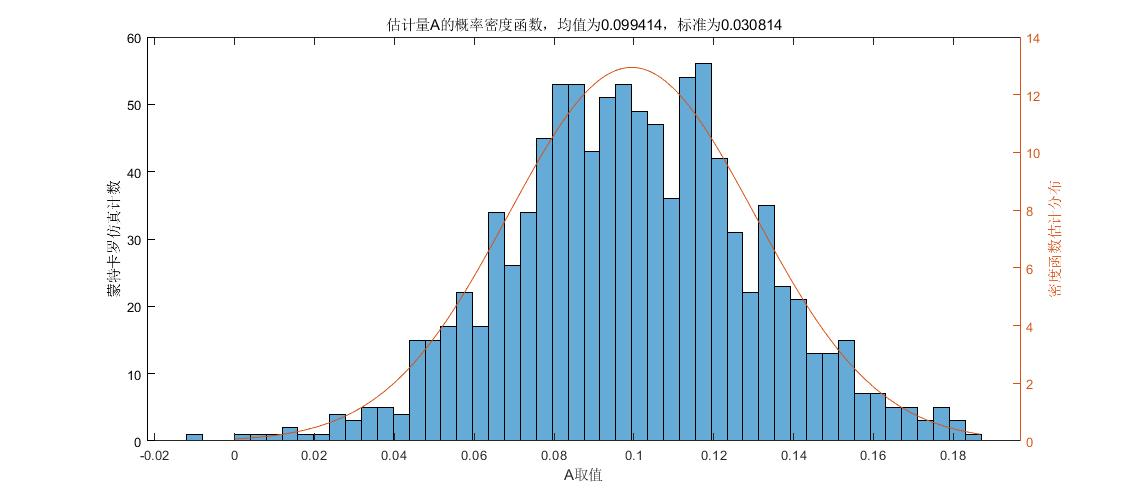
\includegraphics[scale=0.4]{fig2.1.jpg}
	\caption{估计量\(\hat{A}\)的PDF}
	\label{1.2.1}
\end{figure}

\subsubsection*{(2)估计量\(\hat{A}\)和\(\sigma^2\)的性能}


进行一次仿真计算,得到\(E[\hat{A}]=0.10055\),\(var(\hat{A})=0.00093\)。
估计量\(\hat{A}\)的PDF仿真结果如图2.2。
\begin{figure}[H]
	\centering
	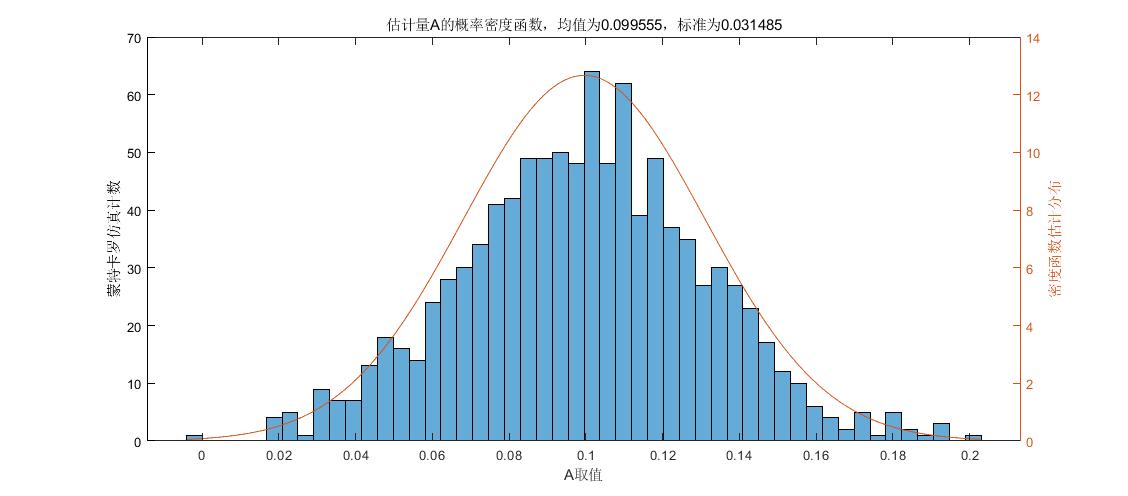
\includegraphics[scale=0.4]{fig2.2.jpg}
	\caption{估计量\(\hat{A}\)的PDF}
	\label{1.2.2}
\end{figure}

得到\(E[\sigma^2]=1.00011\),\(var(\sigma^2)=0.00196\)。
估计量\(\sigma^2\)的PDF仿真结果如图2.3。
\begin{figure}[H]
	\centering
	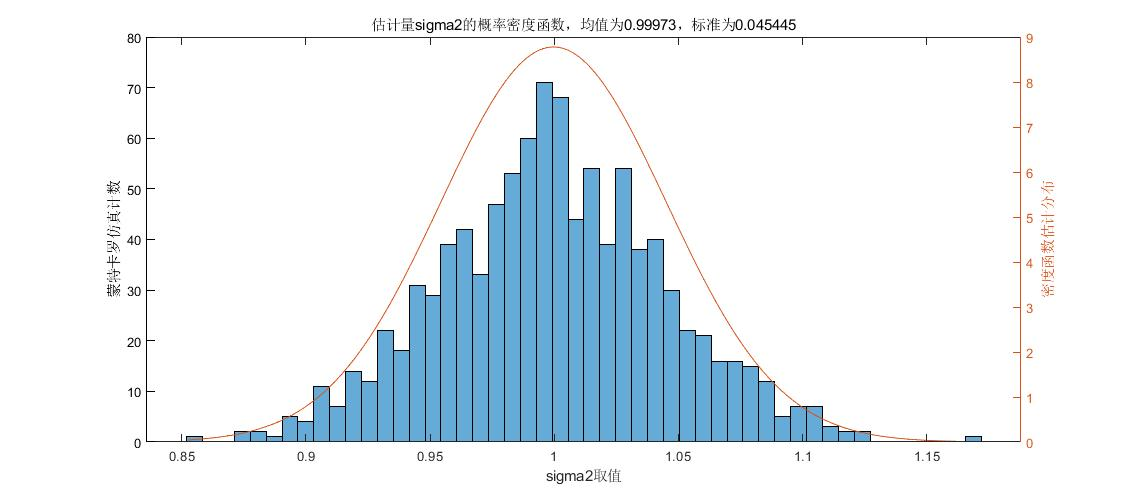
\includegraphics[scale=0.4]{fig2.3.jpg}
	\caption{估计量\(\sigma^2\)的PDF}
	\label{1.2.3}
\end{figure}

\subsubsection*{(3)估计量性能随N的变化讨论}


当N从1至1000变化时,估计量\(\hat{A}\)和估计量\(\sigma^2\)的期望变化如图2.4。
\begin{figure}[H]
	\centering
	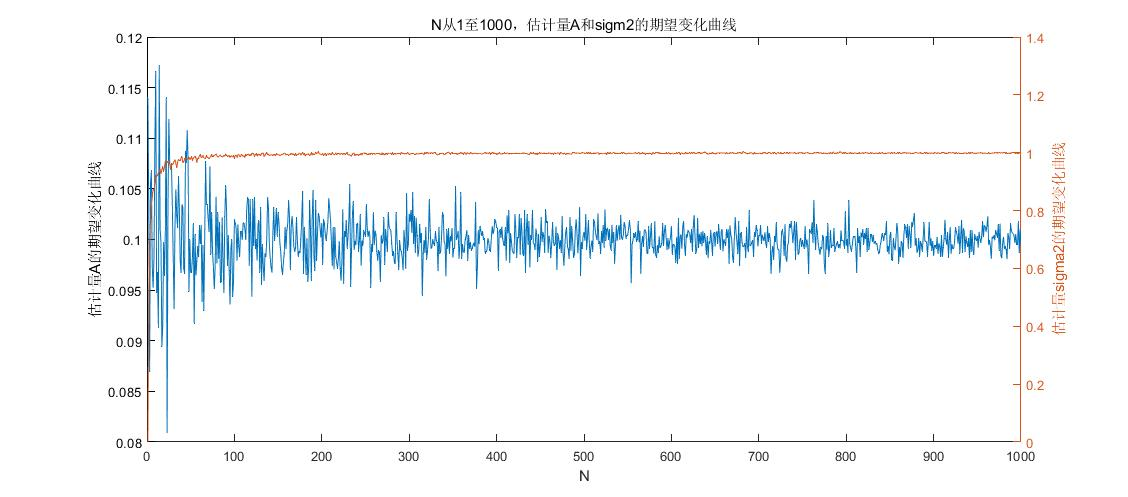
\includegraphics[scale=0.4]{fig2.4.jpg}
	\caption{估计量\(\hat{A}\)和\(\sigma^2\)的期望随N增长的变化曲线}
	\label{2.4}
\end{figure}
从图2.4中可以看出,当N等于1000时,估计量\(\hat{A}\)和\(\sigma^2\)的期望接近于各自真值,
这说明从无偏性角度来看,估计量\(\hat{A}\)和\(\sigma^2\)都应当都是无偏估计。

当N从1至1000变化时,估计量\(\hat{A}\)和估计量\(\sigma^2\)的方差的自然对数
(即ln(var(\(\hat{A}\)))和ln(var(\(\sigma^2\))))变化如图2.5。

\begin{figure}[H]
	\centering
	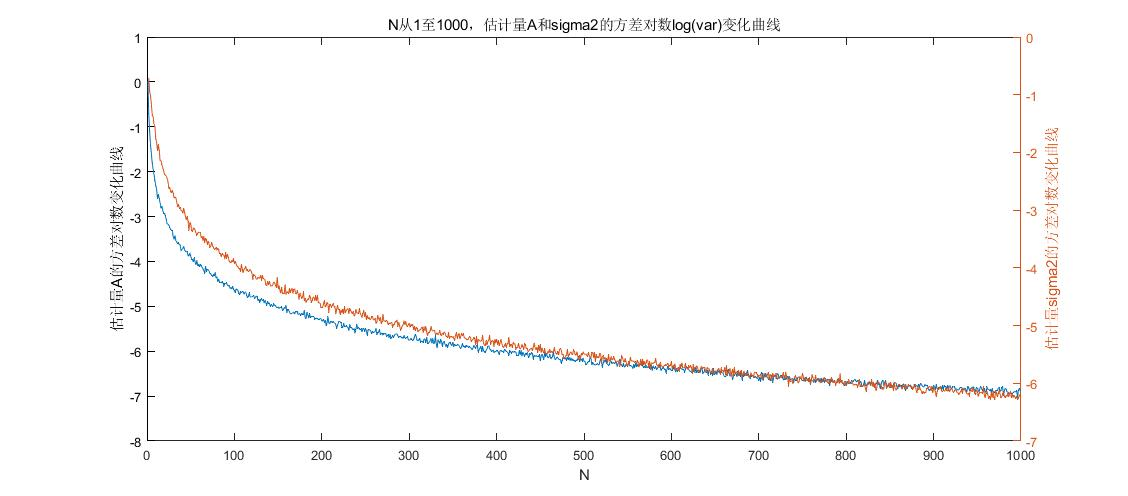
\includegraphics[scale=0.4]{fig2.5.jpg}
	\caption{估计量\(\hat{A}\)和\(\sigma^2\)的方差自然对数ln(var)随N增长的变化曲线}
	\label{2.5}
\end{figure}

由于估计量\(\hat{A}\)和估计量\(\sigma^2\)的收敛速度均较快,为对比明显起见,
图2.5中纵轴均取估计量方差的自然对数。从图2.5可以看出,随着N的增大,
估计量\(\hat{A}\)和估计量\(\sigma^2\)的方差均逐渐减小,且收敛速度接近。
这说明从有效性角度来看,估计量\(\hat{A}\)和估计量\(\sigma^2\)有效性接近。

\subsection{第三题:正弦信号参数估计的CRLB}
假定雷达接收信号可以表示为\(s=Acos(2\pi fn+\varphi)+w(n),n=1,…,N\),N为观测次数
,\(w(n)\sim\mathcal{N}(0,\sigma^2)\)。

(1)A、\(\sigma^2\)已知,均为确定参数,\(f\)未知,\(0<f<\frac{1}{2}\)。试推导\(f\)估计的CRLB
,采用MATLAB画出CRLB随频率、信噪比 、观测次数的变化曲线。

(2)若A、\(\varphi\)、\(f\)均未知,试推导\(f\)估计的CRLB,采用MATLAB画出CRLB随其影响参数的
变化曲线。并对比分析此时\(f\)估计方差的CRLB与第(1)问中\(f\)估计方差的CRLB。

(3)若噪声\(w(n)\)服从瑞利分布,噪声平均功率与高斯分布情况下相同,试再次分析
第(1)、(2)问中参数估计的CRLB。并分析导致CRLB差异的原因。

\subsubsection*{(1) A、\(\sigma^2\)已知,均为确定参数,\(f\)未知}

已知\(x[n]=s[n;\theta]+w[n]\),其中\(s=Acos(2\pi f n +\varphi + w(n))\),
n=1,…,N,\(w(n)\sim \mathcal{N} (0,\sigma^2)\)。极大似然函数

\begin{align*}
	p(\mathbf{x};\theta)=(\frac{1}{2\pi \sigma^2})^{\frac{N}{2}}
	\exp\{ -\frac{1}{2\sigma^2}\sum_{n=0}^{N-1}(x[n]-s[n;\theta])^2 \}
\end{align*}
一次求导得到
\begin{align*}
	\frac{\partial p(\mathbf{x};\theta)}{\partial \theta}=
	\frac{1}{\sigma^2}\sum_{n=0}^{N-1}(x[n]-s[n;\theta])\frac{\partial s[n;\theta]}{\partial\theta}
\end{align*}
二次求导得到
\begin{align*}
	\frac{\partial^2 p(\mathbf{x};\theta)}{\partial \theta}=
	\frac{1}{\sigma^2}\sum_{n=0}^{N-1}\{(x[n]-s[n;\theta])
	\frac{\partial^2 s[n;\theta]}{\partial\theta^2}
	-\left(\frac{s[n;\theta]}{\theta}\right)^2\}
\end{align*}
取数学期望后得到
\begin{align*}
	E\left(\frac{\partial^2 p(\mathbf{x};\theta)}{\partial \theta}\right)=
	-\frac{1}{\sigma^2}\sum_{n=0}^{N-1}
	\left(\frac{s[n;\theta]}{\theta}\right)^2
\end{align*}
将\(s=Acos(2\pi f n +\varphi + w(n))\)带入得到
\begin{align*}
	E\left(\frac{\partial^2 p(\mathbf{x};\theta)}{\partial \theta}\right)=
	-\frac{A^2}{\sigma^2}\sum_{n=0}^{N-1}
	\left[2\pi f n \sin(2\pi f n+\varphi)\right]^2
\end{align*}
得到CRLB为
\begin{align*}
	var(\hat{f})
	\geq \frac{\sigma^2}{A^2 \sum_{n=0}^{N-1}
		\left[2\pi f n \sin(2\pi f n+\varphi)\right]^2}
	=	\frac{1}{\eta ^2 \sum_{n=0}^{N-1}
		\left[2\pi f n \sin(2\pi f n+\varphi)\right]^2}
\end{align*}

\subsubsection*{(2) A、\(\varphi\)、\(f\)均未知}
如果A、\(\varphi\)、\(f\)均未知,估计量\(\boldsymbol{\theta}=[Af\phi]^T\),由于

\begin{align*}
	[\mathbf{I}(\boldsymbol{\theta})]_{ij}=\frac{1}{\sigma^2}\sum_{n=0}^{N-1}
	\frac{\partial s[n;\boldsymbol{\theta}]}{\partial \theta_i}
	\frac{\partial s[n;\boldsymbol{\theta}]}{\partial \theta_j}
\end{align*}

如果\(f\)不靠近0或者1/2,对于\(i=0,1,2\)

\begin{align*}
	\frac{1}{N^{i+1}}\sum_{n=0}^{N-1}n^i\sin(4\pi f n+2\varphi)\approx 0 \\
	\frac{1}{N^{i+1}}\sum_{n=0}^{N-1}n^i\cos(4\pi f n+2\varphi)\approx 0
\end{align*}

利用近似,并且令\(\alpha=2\pi fn+\varphi\),得到

\begin{align*}
	[\mathbf{I}(\boldsymbol{\theta})]_{11}
	 & =\frac{1}{\sigma^2}\sum_{n=0}^{N-1}\cos^2 \alpha
	=\frac{1}{\sigma^2}\sum_{n=0}^{N-1}\left(\frac{1}{2}-\frac{1}{2}\cos2\alpha\right)
	\approx\frac{N}{2\sigma^2}                                           \\
	[\mathbf{I}(\boldsymbol{\theta})]_{12}
	 & =-\frac{1}{\sigma^2}\sum_{n=0}^{N-1}A2\pi n \cos\alpha \sin\alpha
	=-\frac{\pi A}{\sigma^2}\sum_{n=0}^{N-1}n\sin 2\alpha
	\approx 0                                                            \\
	[\mathbf{I}(\boldsymbol{\theta})]_{13}
	 & =-\frac{1}{\sigma^2}\sum_{n=0}^{N-1}A\cos\alpha \sin\alpha
	=-\frac{A}{2\sigma^2}\sum_{n=0}^{N-1}\sin 2\alpha
	\approx 0                                                            \\
	[\mathbf{I}(\boldsymbol{\theta})]_{22}
	 & =\frac{1}{\sigma^2}\sum_{n=0}^{N-1}A^2(2\pi n)^2\sin^2 \alpha
	=\frac{(2\pi A)^2}{\sigma^2}\sum_{n=0}^{N-1}n^2\left(\frac{1}{2}-
	\frac{1}{2}\cos2\alpha\right)                                        \\
	 & \approx\frac{(2\pi A)^2}{2\sigma^2}\sum_{n=0}^{N-1}n^2            \\
	[\mathbf{I}(\boldsymbol{\theta})]_{23}
	 & =\frac{1}{\sigma^2}\sum_{n=0}^{N-1}(2\pi nA)^2 \sin^2\alpha
	\approx \frac{\pi A^2}{\sigma^2}\sum_{n=0}^{N-1}n                    \\
	[\mathbf{I}(\boldsymbol{\theta})]_{33}
	 & =\frac{1}{\sigma^2}\sum_{n=0}^{N-1}A^2\sin^2 \alpha
	\approx \frac{NA^2}{2\sigma^2}
\end{align*}

Fisher信息矩阵为

\begin{align*}
	\mathbf{I}(\boldsymbol{\theta})=\frac{1}{\sigma^2}
	\begin{bmatrix}
		\frac{N}{2} & 0                             & 0                        \\
		0           & 2\pi^2 A^2\sum_{n=0}^{N-1}n^2 & \pi A^2\sum_{n=0}^{N-1}n \\
		0           & \pi A^2\sum_{n=0}^{N-1}n      & \frac{NA^2}{2}
	\end{bmatrix}
\end{align*}

从而得到

\begin{align*}
	var(\hat{f}) \geq \frac{12}{(2\pi)^2\eta N (N^2-1)}
\end{align*}

其中\(\eta=A^2/(2\sigma^2)\)是SNR。
\subsubsection*{(3) \(w(n)\)服从瑞利分布}
假设\(w[n]\)服从瑞利分布,分布函数为

\begin{align*}
	f(x)=\left\{
	\begin{matrix}
		\frac{x}{\sigma_0^2} \exp -\frac{x^2}{2\sigma_0 ^2} & x = 0 \\
		0                                                   & x<0
	\end{matrix}
	\right.
\end{align*}

期望为\(\sqrt{\frac{\pi}{2}}\sigma_0\),方差为\((2-\sqrt{\frac{\pi}{2}})\sigma_0\)。
似然函数变为

\begin{align*}
	p(\mathbf{x};\theta)=\prod_{n=0}^{N-1}\frac{x[n]-s[n;\theta]}{\sigma_0^2}
	\exp \left\{ -\frac{(x[n]-s[n;\theta])^2}{2\sigma_0^2}\right\}
\end{align*}

对数似然函数

\begin{align*}
	\ln p(\mathbf{x};\theta)=-2N\ln \sigma_0+\sum_{n=0}^{N-1}\ln (x[n]-s[x,\theta])
	-\frac{(x[n]-s[n;\theta])^2}{2\sigma^2}
\end{align*}

按照(1)中条件,
对对数似然函数求一阶导

\begin{align*}
	\frac{\partial \ln p(\mathbf{x};\theta)}{\partial \theta}
	 & =\sum_{n=0}^{N-1}\frac{-1}{x[n]-s[n;\theta]}\frac{\partial s[n;\theta]}{\partial \theta}
	+\frac{x[n]-s[n;\theta]}{\sigma_0^2}\frac{\partial s[n;\theta]}{\partial \theta}            \\
	 & =\sum_{n=0}^{N-1}\frac{\partial s[n;\theta]}{\partial \theta}
	\left[\frac{x[n]-s[n;\theta]}{\sigma_0^2}-\frac{1}{x[n]-s[n;\theta]}\right]
\end{align*}

二阶导为

\begin{align*}
	\frac{\partial^2 \ln p(\mathbf{x};\theta)}{\partial \theta^2}=
	\sum_{n=0}^{N-1} & \frac{\partial^2 s[n;\theta]}{\partial \theta^2}
	\left[\frac{x[n]-s[n;\theta]}{\sigma_0^2}-\frac{1}{x[n]-s[n;\theta]}\right]     \\
	                 & -\left(\frac{\partial s[n;\theta]}{\partial \theta}\right)^2
	\left[\frac{1}{\sigma_0^2}+\frac{1}{(x[n]-s[n;\theta])^2}\right]
\end{align*}

由于瑞利分布的均值为\(\sqrt{\frac{\pi}{2}}\sigma_0\),所以

\begin{align*}
	E\left[\frac{\partial^2 \ln p(\mathbf{x};\theta)}{\partial \theta^2}\right]
	=\frac{1}{\sigma_0^2}\sum_{n=0}^{N-1}(\sqrt{\frac{\pi}{2}}-\sqrt{\frac{2}{\pi}})\sigma_0
	\frac{\partial^2 s[n;\theta]}{\partial \theta^2}
	-(\frac{2}{\pi}+1)\left(\frac{\partial s[n;\theta]}{\partial \theta}\right)^2
\end{align*}

将\(s=A\cos (2\pi fn+\varphi)\)带入上式得到

\begin{align*}
	E\left[\frac{\partial^2 \ln p(\mathbf{x};\theta)}{\partial \theta^2}\right]
	=\frac{(2\pi n)^2A^2}{\sigma_0^2}\sum_{n=0}^{N-1}(\sqrt{\frac{2}{\pi}}-
	\sqrt{\frac{\pi}{2}})\frac{\sigma_0}{A}\cos (2\pi fn+\varphi)
	-(\frac{2}{\pi}+1)(\sin 2\pi n+\varphi)^2
\end{align*}

\subsection{第四题:天线阵列信号的信噪比与CRLB}
采用阵列天线对高斯噪声背景下空间电磁波的来波方向进行估计。阵列天线接收信号为:
\(s(t)=A\cos (2\pi ft+\varphi)+w(n)\)。载频\(f=5GHz\),阵列天线各阵元间距为\(\lambda/2\)
,\(\lambda\)为来波波长。阵元数为32。背景噪声\(w(n)\sim \mathcal{N} (0,\sigma^2)\)。
(1)试分析来波从不同方向到达时,阵列天线来波角度估计的CRLB,给出CRLB随相关参数变化的曲线图。
(2)设面阵法向为0度,论:要若对方位向60度的来波,角度估计精度精准偏差不超过1度。在信噪比为5dB
的情况下,阵元至少需要多少个?若阵元数为8,信噪比至少需为多少?
(3)若来波载频为C波段,具体值未知,试讨论阵元间距应该如何设置可使来波角度估计的CRLB较小?

\subsubsection*{(1)分析不同方向来波时,天线角度估计的CRLB}

假定满足平面波假设,则第n个阵元的传播时间为:
\begin{align*}
	t_n=t_0-n\frac{d}{c}\cos \beta \quad n=0,1,\cdots,M-1
\end{align*}
其中,\(t_0\)是第0个阵元的传播时间。因此可得第n个阵元的接收信号:
\begin{align*}
	s_n(t)=A\cos \left[2\pi f(t-t_0+n\frac{d}{c}\cos \beta)+\varphi\right]
\end{align*}
在某一时刻\(t_s\)对阵元的输出采样:
\begin{align*}
	s_n(t_s)=A\cos\left[2\pi (f\frac{d}{c}\cos\beta)n+\phi\right]
\end{align*}
其中\(\phi=\varphi+2\pi f(t_s-t_0)\),由此可得观测模型
\begin{align*}
	x[n]=s_n(t_s)+w[n]\quad n=0,1,\cdots,M-1
\end{align*}
设矢量参数\(\boldsymbol{\theta}=[A,f_s,\phi]^T\),矢量参数变换
\begin{align*}
	\alpha=g(\boldsymbol{\theta}) & =
	\begin{bmatrix}
		A \\\beta\\\phi
	\end{bmatrix}=
	\begin{bmatrix}
		A \\\arccos(\frac{cf_s}{fd})\\\phi
	\end{bmatrix}    \\
	var(\hat{\beta})              & \geq
	\left[\frac{\partial g(\theta)}{\partial \theta}\right]^2_{22}\left[I^{-1}(\theta)\right]_{22}
\end{align*}
因此
\begin{align*}
	var(\hat{\beta})
	 & \geq \frac{12}{(2\pi )\eta M(M^2-1)}\frac{c^2}{f^2d^2\sin^2\beta} \\
	 & =\frac{12\lambda^2}{(2\pi)^2\eta M(M^2-1)d^2\sin^2\beta}          \\
	 & =\frac{1}{2728\eta \pi^2\sin^2\beta}
\end{align*}

\subsubsection*{(2)阵元与信噪比讨论}
由题意
\begin{align*}
	var(\hat{\beta})\leq (\frac{\pi}{180})^2
\end{align*}

当\(\eta=5dB\)时,可得\(M\geq 18\)。当\(M=8\)时,\(\eta\geq 31.678=15dB\)

\subsubsection*{(3)阵元间距设置}

CRLB与着呢元间距成反比关系,故应当尽可能使得阵元间距d更大,相邻阵元间距的接收信号时间差为
\begin{align*}
	\Delta t=\frac{\cos \beta}{c}
\end{align*}

波达角\begin{align*}
	\beta=\arccos \left(\frac{c\Delta t}{d}\right)=\arccos\left(\frac{\lambda\Delta\varphi}{2\pi d}\right)
\end{align*}
为避免产生多值,\(\Delta\varphi\in [-\pi, \pi]\),因此阵列间距\(d\leq \lambda/2\)。故阵元间距应当设置为\(\lambda/2\)

\section{完备性,充分性,正弦信号频率估计}

\subsection{第一题:完备性、充分性与有效性}
什么叫做完备的充分统计量?如何利用完备的充分统计量估计未知参数?由充分统计量是否能够获得MVUE?
获得最大似然估计的途径有哪些?最大似然估计与有效估计量、充分统计量、MVUE之间是否有联系?
可举例验证你的观点。

\subsubsection*{(1)什么叫做完备的充分统计量?}

1.充分性条件:如果\(PDFp(\mathbf{x};\theta)\)能够分解为
\begin{align*}
	p(\mathbf{x};\theta)=g(T(\mathbf{x},\theta))h(\mathbf{x})
\end{align*}
其中g为只是通过\(T(\mathbf{x})\)才与\(\mathbf{x}\)有关的函数,
h只是\(\mathbf{x}\)的函数,那么\(T(\mathbf{x})\)是\(\theta\)的充分统计量。

2.完备性条件:如果对所有的\(\theta\),条件
\begin{align*}
	\int_{-\infty}^{\infty} v(T)p(T;\theta)dT=0
\end{align*}
只对零函数\(v(T)=0\)(对所有的T)满足,那么,我们就说充分统计量是完备的。

\subsubsection*{(2)如何利用完备的充分统计量估计未知参数?}

根据BRLS定理,\(\hat{\theta}\)时\(\theta\)的无偏估计,\(T(z)\)时一个充分统计量,那么\(\hat{\theta}=E(\theta|T(z))\)是\(\theta\)的一个适用的估计量。

\subsubsection*{(3)由充分统计量是否能够获得MVUE?}
根据BRLS定理,如果充分统计量\(T(\mathbf{x})\)是完备的,那么它就是MVUE。
1.利用Neyman-Fisher因子分解定理来求一个\(\theta\)的统计量,即\(T(\mathbf{x})\);

2.确定充分统计量是否完备,如果是,继续往下进行;否则这个方法不能使用;
3.求一个充分统计量的函数,以此来得到一个无偏估计量\(\hat{\theta}=g(T(\mathbf{x}))\),
那么\(\hat{\theta}\)就是MVUE。或者,计算\(\hat{\theta}=E(\check{\theta}|T(\mathbf{\theta}))\)
,其中\(\check{\theta}\)是任意无偏估计量。

\subsubsection*{(4)获得最大似然估计的途径有哪些?}
1.写出似然函数,求出使得似然函数最大的估计量\(\hat{\theta}\)

2.已知充分统计量\(T(\mathbf{x})\),根据Neyman-Fisher因子分解定理,似然函数最大化等价于\(g(T(\mathbf{x},\theta))\)的最大化,因此求得使\(g(T(\mathbf{x},\theta))\)关于\(\theta\)最大化的估计量即为MLE。

\subsubsection*{(5)最大似然估计与有效估计量、充分统计量、MVUE之间是否有联系?}
有效估计量:无偏且达到CRLB的估计量。

充分统计量:包含待估计量所有信息的统计量。

MVUE:在无偏估计的前提下,使得方差最小的估计量。

MVUE估计量和有效估计量都是无偏的,但MVUE不一定是有效估计量(见教材图3.2);
根据教材定理7.1,最大似然估计量可以视为渐进无偏的和渐进达到CRLB,因此它是渐进有效的;
根据Neyman-Fisher因子分解定理,对于充分统计量\(T(\mathbf{x})\),PDF可以分解为
\(p(T(\mathbf{x});\theta)=g(T(\mathbf{x},\theta))h(\mathbf{x})\),
求MLE时,使似然函数最大化,等价于使\(g(T(\mathbf{x},\theta))\)关于\(\theta\)求得极大值,
因此,MLE是充分统计量\(T(\mathbf{x})\)的函数。

\subsection{第二题:正弦信号的参数估计}
考虑高斯噪声中正弦信号参数估计问题。观测模型为
\begin{align*}
	x_n=A\cos2\pi f_0 n+w_n,n=0,1,…,N-1
\end{align*}
其中\(w_n\)为零均值高斯噪声。

\subsubsection*{(1)当\(w_n\overset{i.i.d}{\sim} N(0,\sigma^2)\),\(f_0\)、\(\sigma^2\)均已知,你认为可以用哪些方法对参数A进行估计?}

方法一:利用RBLS定理求解。观测信号的似然函数为
\begin{align*}
	p(\mathbf{x};A)=\frac{1}{(2\pi \sigma ^2)^{\frac{N}{2}}}\exp\left\{ -\frac{1}{2\sigma^2}
	\sum_{n=0}^{N-1}(x_n-A\cos2\pi f_0 n)^2	\right\}
\end{align*}
可变换为
\begin{align*}
	p(\mathbf{x};A) & =\frac{1}{(2\pi \sigma^2)^{\frac{N}{2}}}\exp\left\{-\frac{1}{2\sigma^2}
	\sum_{n=0}^{N-1}(x_n^2 +A^2\cos^2 2\pi f_0 n-2x_n A cos 2\pi f_0 n)\right\}               \\
	                & =\frac{1}{(2\pi \sigma^2)^{\frac{N}{2}}}\exp\left\{-\frac{1}{2\sigma^2}
	\sum_{n=0}^{N-1}(A^2\cos^2 2\pi f_0 n-2x_n A cos 2\pi f_0 n)\right\}
	\exp\left\{-\frac{1}{2\sigma^2}\sum_{n=0}^{N-1}x_n^2\right\}
\end{align*}
令
\begin{align*}
	h(x) & =\exp\left\{-\frac{1}{2\sigma^2}\sum_{n=1}^{N-1}x_n^2\right\} \\
	T(x) & =\sum_{n=0}^{N-1}x_n \cos 2\pi f_0 n
\end{align*}
其中
\begin{align*}
	E[T(x)] & =\left[\sum_{n=0}^{N-1}(A\cos 2\pi f_0 n+w_n)\cos 2\pi f_0 n \right] \\
	        & =A\sum_{n=0}^{N-1}\cos^2 2\pi f_0 n
\end{align*}
令
\begin{align*}
	\hat{A}=\frac{\sum_{n=0}^{N-1}x_n \cos 2\pi f_0 n}{\sum_{n=0}^{N-1}\cos^2 2\pi f_0 n}
\end{align*}
则A的估计量\(\hat{A}\)满足\(E[\hat{A}]=A\)。

方法二:利用最大似然法求解。对观测信号的似然函数取对数
\begin{align*}
	\ln p(\mathbf{x};A)=-\frac{N}{2}\ln (2\pi \sigma^2)-
	\frac{1}{2\sigma^2}\sum_{n=0}^{N-1}(x_n-A\cos 2\pi f_0 n)^2
\end{align*}
求导得
\begin{align*}
	\frac{\partial\ln p(\mathbf{x};A)}{\partial A}=-\frac{1}{\sigma^2}
	\sum_{n=0}^{N-1}(x_n-A\cos2\pi f_0 n)\cos(2\pi f_0 n)
\end{align*}
令上式等于零,得
\begin{align*}
	\sum_{n=0}^{N-1}x_n\cos(2\pi f_0 n) & =\sum_{n=0}^{N-1}A\cos(2\pi f_0 n)cos(2\pi f_0 n) \\
	\sum_{n=0}^{N-1}x_n\cos(2\pi f_0 n) & =A\sum_{n=0}^{N-1}\cos^2(2\pi f_0 n)
\end{align*}
估计量\(\hat{A}\)为
\begin{align*}
	\hat{A}=\frac{\sum_{n=0}^{N-1}x_n \cos 2\pi f_0 n}{\sum_{n=0}^{N-1}\cos^2 2\pi f_0 n}
\end{align*}

方法三:利用BLUE求解。对于观测量\(x_n=A\cos(2\pi f_0 n)+w_n\)
\begin{align*}
	E[x_n]=A\cos(2\pi f_0 n)
\end{align*}
令\(E[x_n]=s[n]A\),即\(s[n]=\cos 2\pi f_0 n\),则BLUE为
\begin{align*}
	\hat{A}=\frac{\mathbf{s}^TC^{-1}x}{\mathbf{s}^TC^{-1}s}
\end{align*}
其中\(s=[s(1),s(2),\ldots,s(n-1)]^T\),又因为\(w_n\)是方差为\(\sigma^2\)的零均值高斯噪声,
则\(\mathbf{C}^{-1}=\frac{1}{\sigma^2}\),所以估计量可以表示为
\begin{align*}
	\hat{A}=\frac{\mathbf{s}^TC^{-1}x}{\mathbf{s}^TC^{-1}s}
	=\frac{\mathbf{s}^Tx}{\mathbf{s}^Ts}
	=\frac{\sum_{n=0}^{N-1}x_n \cos 2\pi f_0 n}{\sum_{n=0}^{N-1}\cos^2 2\pi f_0 n}
\end{align*}

\subsubsection*{(2)\(A=1,\sigma^2=0.1\)时,绘制频率参数的克拉美-罗下限曲线,
	并解释你观察到的现象。}

首先计算频率的克拉美-罗下限:
\begin{align*}
	\frac{\partial s[n;f_0]}{\partial f_0} & =-2\pi n A\sin(2\pi f_0 n) \\
	var(\hat{f})                           & \geq \frac{\sigma^2}
	{A^2\sum_{n=0}^{N-1}4\pi^2n^2\sin^2(2\pi f_0 n)}
	=\frac{\sigma^2}
	{\frac{A^2}{2}\sum_{n=0}^{N-1}4\pi^2n^2(1-\cos(4\pi f_0 n))}
\end{align*}

由仿真结果可以看出,CRLB在\(f_0=0\)或0.5时趋向无穷大,这是由于分母值为零,此时估计性能最差。
而随着数据长度的增加,CRLB总体在变小,且震荡越来越剧烈,这时由于分母值与N有关,N越大,
信号随位置参数的变换率越大,CELB越小,估计的精度越好。

\begin{figure}[H]
	\centering
	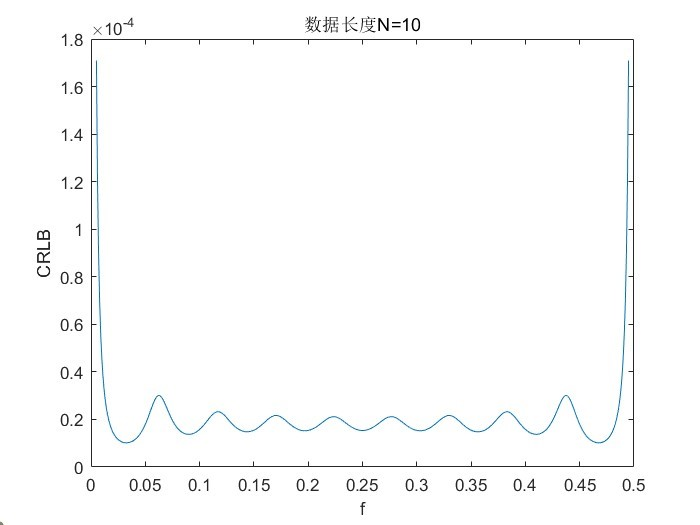
\includegraphics[scale=0.7]{fig1.jpg}
	\caption{数据长度N=10时的CRLB}
	\label{2.2.1}
\end{figure}

\begin{figure}[H]
	\centering
	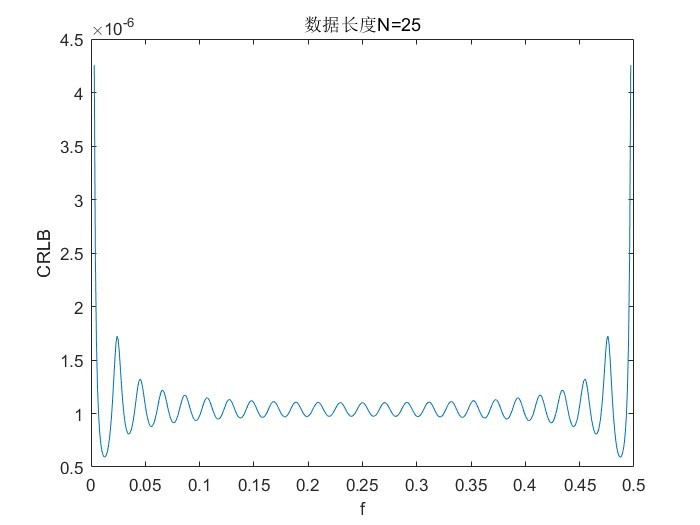
\includegraphics[scale=0.7]{fig2.jpg}
	\caption{数据长度N=25时的CRLB}
	\label{2.2.2}
\end{figure}

\begin{figure}[H]
	\centering
	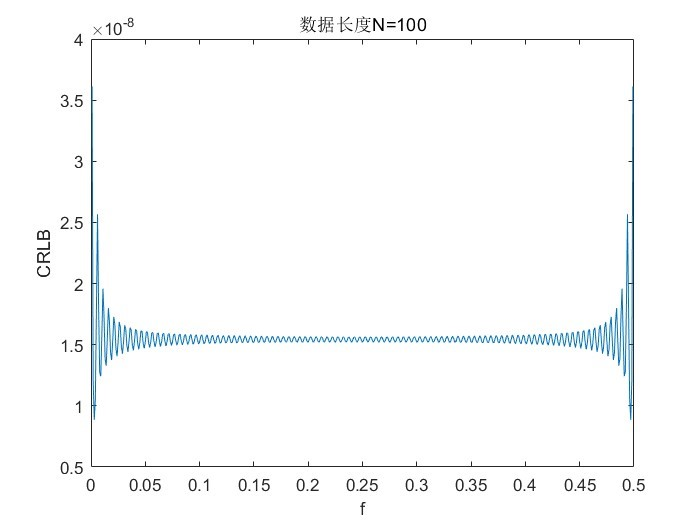
\includegraphics[scale=0.7]{fig3.jpg}
	\caption{数据长度N=100时的CRLB}
	\label{2.2.3}
\end{figure}

\subsubsection*{(3)\(A=1,f_0=0.25,f_0=0.05\)时,分别对频率参数的最大似然估计进行仿真,绘制参数估计性能随样本量、信噪比的变化曲线,
	并与克拉美-罗下限进行对比;分析验证最大似然估计的渐进性能。}

当\(A=1\)时,极大似然函数为
\begin{align*}
	p(\mathbf{x};f_0)=\frac{1}{(2\pi \sigma^2)^{\frac{N}{2}}}
	\exp\left\{-\frac{1}{2\sigma^2}\sum_{n=0}^{N-1}\left[x[n]-\cos2\pi f_0n\right]^2\right\}
\end{align*}
使得似然函数最大,等价于使指数项
\begin{align*}
	J(f_0)=\sum_{n=0}^{N-1}\left[x[n]-\cos2\pi f_0n\right]^2
\end{align*}
最小。对于集合\((0,1/2)\)内的所有\(f_0\),利用网格搜索法,可以求出\(J(f_0)\)的最小值,这时的\(f_0\)即为MLE。

\subsubsection*{(4)如果\(w_n\)为零均值高斯色噪声,可用如下AR模型描述
	\begin{align*}
		w_n=aw_{n-1}+e_n
	\end{align*}
	其中,\(e_n\overset{i.i.d}{\sim}N(0,\sigma_e^2),a=0.8,A=1\),试问什么情况下能够获得更准确的频率参数估计?
	试与白噪声的情况进行比较(相同的噪声方差下)。}

根据递推关系,\(w_n=aw_{n-1}+e_n\),可知
\(E(w_n)=aE(w_{n-1})\),\(var(E_n)=a^2var(E_{n-1})+\sigma_e^2\),当n足够大时,
\(E(w_n)=\frac{0}{1-a}=0\),\(var(w_n)=\frac{\sigma_e^2}{1-a^2}=\frac{\sigma_e^2}{0.36}\)。

根据中心极限定理可知,当n足够大时,\(w_n\sim\mathcal{N}(0,\frac{\sigma_e^2}{0.36})\)。
由\(e_n\)相互独立可知\(w_n\)相互独立。

问题等价于,当\(w_n\overset{i,i,d}{\sim}\mathcal{N}\left(0,\left( \frac{\sigma_e}{0.6}\right)^2\right)\)时,
求\(x_n=\cos2\pi f_0 n +w_n\)更准确的频率估计。

似然函数为
\begin{align*}
	p(\mathbf{x};f_0) & =\frac{1}{(2\pi \sigma^2)^{\frac{N}{2}}}
	\exp\left\{-\frac{1}{2\sigma^2}\sum_{n=0}^{N-1}\left[x[n]-\cos2\pi f_0n\right]^2\right\} \\
	                  & =\frac{1}{(2\pi \sigma^2)^{\frac{N}{2}}}
	\exp\left\{-\frac{1}{2\sigma^2}\left[\sum_{n=0}^{N-1}x^2[n]-
	2\sum_{n=0}^{N-1}x[n]\cos2\pi f_0 n+\sum_{n=0}^{N-1}\cos^22\pi f_0 n
	\right]\right\}                                                                          \\
	                  & =\frac{1}{(2\pi \sigma^2)^{\frac{N}{2}}}
	\exp\left[-\frac{1}{2\sigma^2}\sum_{n=0}^{N-1}x^2[n]\right]
	\exp\left\{-\frac{1}{2\sigma^2}\left[-
	2\sum_{n=0}^{N-1}x[n]\cos2\pi f_0 n+\sum_{n=0}^{N-1}\cos^22\pi f_0 n
	\right]\right\}
\end{align*}
其中,\(\sigma=\frac{\sigma_e}{0.6}\)。由于有\(\sum_{n=0}^{N-1}x[n]\cos2\pi f_0 n\)项,且其中\(f_0\)是未知的,
所以不能用Neyman-Fisher因子分解定理,即无法求出\(f_0\)的充分统计量,这时应使用最大似然估计。
要使似然函数
\begin{align*}
	p(\mathbf{x};f_0)=\frac{1}{(2\pi \sigma^2)^{\frac{N}{2}}}
	\exp\left\{-\frac{1}{2\sigma^2}\sum_{n=0}^{N-1}\left[x[n]-\cos2\pi f_0n\right]^2\right\}
\end{align*}
最大,等价于使指数项\(J(f_0)=\sum_{n=0}^{N-1}\left(x[n]-\cos2\pi f_0 n\right)^2\)最小。
对于集合\((0,1/2)\)内的所有\(f_0\),利用网格搜索法,可以求出\(J(f_0)\)的最小值,这时的\(f_0\)即为MLE。

\begin{figure}[H]
	\centering
	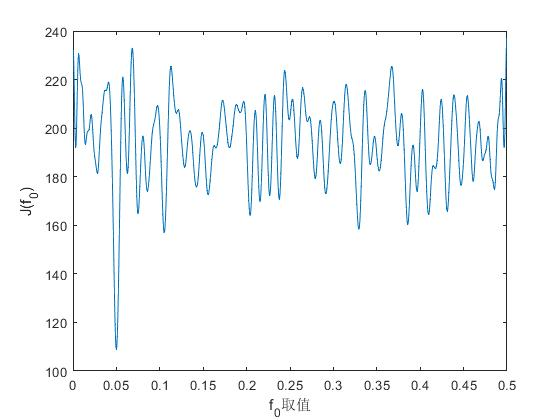
\includegraphics[scale=0.5]{fig4.jpg}
	\caption{通过J的最小值寻找\(f_0\)的MLE}
	\label{2.2.4}
\end{figure}

根据频率的CRLB可知
\begin{align*}
	var(\hat{f}) & \geq\frac{\sigma^2}
	{\frac{A^2}{2}\sum_{n=0}^{N-1}4\pi^2n^2(1-\cos(4\pi f_0 n))} \\
	             & =\frac{(\frac{\sigma_e}{0.6})^2}
	{\frac{A^2}{2}\sum_{n=0}^{N-1}4\pi^2n^2(1-\cos(4\pi f_0 n))}
\end{align*}
色噪声与白噪声相比,CRLB变小,估计精度变高。

\section{贝叶斯估计}
\subsection{第一题:贝叶斯估计基本概念}
获得贝叶斯估计的准则有哪些?先验信息通常如何确定?什么是无信息先验?以观测模型\(z=A+w\)为例,
其中观测噪声\(w\sim \mathcal{N}(0,\sigma^2)\)且与A相互独立。如果对待估参数A没有更多的知识,
你认为可以如何处理?如果要估计的参数是\(\beta=e^A\)时,情况又如何?

\subsubsection*{(1)获得贝叶斯估计的准则有哪些?}

获得贝叶斯估计的准则有最大后验概率、最小均方(MMSE,也称条件均值)、条件中位数估计、
线性最小均方估计

\subsubsection*{(2)先验信息通常如何确定?}

先验信息通常建立在物理约束规律之上。一般,如果待估计量知道其取值范围,
则待估计量先验概率密度选择这个范围上的均匀分布。

\subsubsection*{(3)由什么是无信息先验?}

无信息先验是对于确定性参数利用贝叶斯方法估计时(确定性参数估计通常不采用贝叶斯估计而采用最大似然估计),
先验PDF不含信息量,不向问题增加任何信息。

\subsubsection*{(4)以观测模型\(z=A+w\)为例,
	其中观测噪声\(w\sim \mathcal{N}(0,\sigma^2)\)且与A相互独立。如果对待估参数A没有更多的知识,
	你认为可以如何处理?如果要估计的参数是\(\beta=e^A\)时,情况又如何?}

如果对参数A没有更多的知识,可以考虑将其视为位置常数,采用最大似然估计、利用充分统计量求最小方差无偏估计、线性最小方差无偏估计等方法。此时参数A的最优估计量为\(\hat{A}=\overline{z}\)。

若要采用贝叶斯估计方法,可采用位置参数的无信息先验方法。容易验证此时A是一个位置参数,所以取广义先验分布\(p(A)=1\),利用贝叶斯公式和充分统计量\(\overline{z}\)计算后验分布为
\begin{align*}
	p(A|\overline{z})
	 & =\frac{p(\overline{z},A)}{p(\overline{z})}                                                 \\
	 & =\frac{p(\overline{z}|A)p(A)}{\int_{-\infty}^{\infty}p(\overline{z}|A)p(A)dA}              \\
	 & =\frac{1}{\sqrt{2\pi \sigma^2/N}}\exp\left[-\frac{1}{2\sigma^2/N}(\overline{z}-A)^2\right]
\end{align*}

故参数A的后验分布为:\(A\sim \mathcal{N}(\overline{z},\sigma^2/N)\),若采用最大后验概率准则,可得到A的估计量为\(\hat{A}_{map}=\overline{z}\)

\subsubsection*{(5)如果要估计的参数是\(\beta=e^A\)},同样可以考虑将其视为未知常数,采用经典估计方法进行估计,如最大似然估计可利用其不变性得到\(\hat{A}_{ml}=e^{\overline{z}}\)。

若要采用贝叶斯估计方法,仍取广义先验分布\(p(A)=1\),考虑最大后验概率准则
\begin{align*}
	\hat{\beta}_{map}=arg\underset{\beta}{\max}p(z|\beta)p(\beta)=arg\underset{\beta}{\max}(\ln p(z|\beta)+\ln p(\beta))
\end{align*}
其中
\begin{align*}
	p(z|\beta)
	 & =\frac{1}{(2\pi \sigma^2)^{N/2}}
	\exp\left[-\frac{1}{2\sigma^2}\sum_{i=0}^{N-1}(z_i-\ln\beta)^2\right] \\
	p(\beta)
	 & =\frac{d\ln\beta}{d\beta}\cdot p_A(\ln \beta)=\frac{1}{\beta}
\end{align*}
从而有,
\begin{align*}
	\hat{\beta}_{map}=arg\underset{\beta}{\max}\left[\ln\beta+
		\frac{1}{2\sigma^2}\sum_{i=0}^{N-1}(z_i-\beta)^2\right]
	=e^{\overline{z}-\sigma^2/N}
\end{align*}

\subsection{第二题:先验概率、后验概率与最小均方估计}
贝叶斯估计器与后验分布\(p(A|\mathbf{z})\)有什么关系?是否可以用后验方差来评价最小均方误差估计器的性能?
参数A的先验方差、后验方差以及贝叶斯最小均方误差之间有无关系?

\subsubsection*{(1)贝叶斯估计器与后验分布\(p(A|\mathbf{z})\)有什么关系?}
由于A是一个随机变量,所以期望运算是对联合PDF\(p(\mathbf{z},A)\)求取的,这是贝叶斯估计与经典估计本质上的不同,
贝叶斯均方误差定义为:
\begin{align*}
	Bmse(\hat{A})=\int\int(A-\hat{A})^2 p(\mathbf{z},A)d\mathbf{z}dA
\end{align*}

依据贝叶斯原理,我们有:
\begin{align*}
	p(\mathbf{z},A)=p(A|\mathbf{z})p(\mathbf{z})
\end{align*}
所以贝叶斯均方误差由可以写成:
\begin{align*}
	Bmse(\hat{A})=\int \left[\int (A-\hat{A})^2 p(A|\mathbf{z})dA\right]p(\mathbf{z})d\mathbf{z}
\end{align*}
又由于对所有的\(\mathbf{z}\)而言都有\(p(\mathbf{z})>0\),如果括号内的积分对每个\(\mathbf{z}\)都最小,
那么贝叶斯均方误差将达到最小:
\begin{align*}
	\frac{\partial}{\partial \hat{A}}\int (A-\hat{A})^2 p(A|\mathbf{z})dA
	 & =\int \frac{\partial}{\partial \hat{A}}(A-\hat{A})^2 p(A|\mathbf{z})dA \\
	 & =\int -2(A-\hat{A})p(A|\mathbf{z})dA                                   \\
	 & =-2\int Ap(A|\mathbf{z})dA+2\int \hat{A}p(A|\mathbf{z})dA
\end{align*}
令一阶导数等于零,可以得到:
\begin{align*}
	\hat{A}=\int Ap(A|\mathbf{z})dA=E(A|\mathbf{z})
\end{align*}

因此,贝叶斯均方误差最小的估计量是后验PDF\(p(A|\mathbf{z})\)的均值。

另外,贝叶斯最大后验改立估计是后验分布的最大值,贝叶斯条件中位数估计是
后验分布的中值,依次满足:
\begin{align*}
	\hat{A}_{map} & =\arg \underset{A}{\max} p(A|\mathbf{z})          \\
	\int_{-\infty}^{\hat{A}_{med}} p(A|\mathbf{z})dA
	              & =\int^{+\infty}_{\hat{A}_{med}} p(A|\mathbf{z})dA
\end{align*}

\subsubsection*{(2)是否可以用后验方差来评价最小均方误差估计器的性能?}
后验方差的定义为:
\begin{align*}
	Var(A|\mathbf{z})=\int (A-E(A|\mathbf{z}))^2 p(A|\mathbf{z})dA
\end{align*}
根据第一问中\(\hat{A}=E(A|\mathbf{z})\),有
\begin{align*}
	Bmse(\hat{A})
	 & =\int \left[\int (A-\hat{A})^2 p(A|\mathbf{z})dA\right]p(\mathbf{z})d\mathbf{z} \\
	 & =\int Var(A|\mathbf{z})p(\mathbf{z})d\mathbf{z}
\end{align*}
当后验方差\(Var(A|\mathbf{z})\)对所有观测\(\mathbf{z}\)都能最小,那么将达到贝叶斯最小均方误差估计。
后验方差越小,贝叶斯均方误差越小,估计器性能越好。

\subsubsection*{(3)参数A的先验方差、后验方差以及贝叶斯最小均方误差之间有无关系?}
根据方差分解公式
\begin{align*}
	Var(X)=Var(E(X|Y))+E(Var(X|Y))
\end{align*}
令\(X=A,Y=\mathbf{z}\)可得
\begin{align*}
	Var(A)=Var(E(A|\mathbf{z}))+E(Var(A|\mathbf{z}))=Bmse(\hat{A})+E(Var(A|\mathbf{z}))
\end{align*}
即先验方差等于贝叶斯均方误差与后验方差均值之和,因此一般而言,先验方差要大于等于后验方差与贝叶斯最小均方误差之和。

针对习题10.10:

条件PDF为:
\begin{align*}
	p(\mathbf{x}|\theta)=\prod_{n=0}^{N-1}p(\mathbf{x}[n]|\theta)=
	\left\{
	\begin{matrix}
		\theta^N\exp(-\theta \sum_{n=0}^{N-1} x[n]) & ,min(x[n])>0 \\
		0                                           & ,other
	\end{matrix}
	\right.
\end{align*}
后验PDF为
\begin{align*}
	p(\theta|\mathbf{x})=\frac{p(\mathbf{x},\theta)}{\int p(\mathbf{x},\theta)d\theta}
	=\frac{\frac{\lambda ^\alpha}{\Gamma(\alpha)}\theta^{N+\alpha-1}
		\exp\left[-\theta (\lambda+\sum_{n=0}^{N-1}x[n])\right]}
	{\frac{\lambda ^\alpha}{\Gamma(\alpha)}\int_0^{\infty}\theta^{N+\alpha-1}
		\exp \left[ -\theta (\lambda+\sum_{n=0}^{N-1}x[n]) \right]}
\end{align*}
根据\(\int_0^{\infty}p(\theta)d\theta=1\)可得
\begin{align*}
	\int_{0}^{\infty} \theta^{\alpha-1}\exp (-\lambda \theta)d\theta=
	\frac{\Gamma(\alpha)}{\lambda^{\alpha}}
\end{align*}
从而有
\begin{align*}
	p(\theta|\mathbf{x})=\left\{
	\begin{matrix}
		\frac{(N\overline{x}+\lambda)^{N+\alpha}}{\Gamma(N+\alpha)}
		\theta^{N+\alpha+1}\exp \left[ -\theta (\lambda+N \overline{x})\right] & ,\theta>0 \\
		0                                                                      & ,others
	\end{matrix}
	\right.
\end{align*}
此时后验PDF与先验PDF形式一样,仍然是一个伽马分布,只是\(\alpha'=\alpha+N,\lambda'=N\overline{x}+\lambda\)。
由伽马分布的方差分布,先验方差为\(\frac{\alpha}{\lambda^2}\),后验方差为\(\frac{\alpha'}{\lambda'^2}\),
贝叶斯最小均方误差等于后验方差对观测\(\mathbf{x}\)的均值:
\begin{align*}
	Bmse(\hat{\theta})=\int Var(\theta|\mathbf{x})p(\mathbf{x})d\mathbf{x}
\end{align*}

\subsection{第三题:线性模型的岭估计}
考虑线性模型参数估计问题
\begin{align*}
	\mathbf{z}=\mathbf{H}\boldsymbol{\theta}+\mathbf{e}
\end{align*}

其中\(\mathbf{z}\in \mathbb{R}^N\)为观测数据矢量,\(\mathbf{H}\in \mathbb{R}^{N\times P},(N>P)\)
为已知测量矩阵,\(\boldsymbol{\theta}\in \mathbb{R} ^P\)为未知参数,\(\mathbf{e}\overset{i.i.d}{\sim}
\mathcal{N}(\mathbf{0},\sigma^2_e \mathbf{I})\)为测量误差。

\subsubsection*{(1)如果\(\mathbf{H}\)满秩,你认为可以如何估计参数\(\theta\)?}

如果\(\mathbf{H}\)满秩,则\(\mathbf{H}^T \mathbf{H}\)可逆。\(PDF\)为
\begin{align*}
	p(\mathbf{z}|\boldsymbol{\theta})
	 & =\frac{1}{(2\pi \sigma_e^2)^{\frac{N}{2}}}
	\exp\left\{-\frac{1}{2\sigma_e^2} \left[\mathbf{z-H}\boldsymbol{\theta}\right]^T
	\left[\mathbf{z-H}\boldsymbol{\theta}\right]\right\} \\
	 & =\frac{1}{(2\pi \sigma_e^2)^{\frac{N}{2}}}
	\exp\left\{-\frac{1}{2\sigma_e^2} \mathbf{z}^T \mathbf{z}\right\}\centerdot
	\exp\left\{-\frac{1}{2\sigma_e^2} \left[-2\boldsymbol{\theta}^T\mathbf{H}^T\mathbf{z}
		+\boldsymbol{\theta}^T\mathbf{H}^T\mathbf{H}\boldsymbol{\theta}\right]\right\}
\end{align*}
利用
\begin{align*}
	\frac{\partial \mathbf{x}^T \mathbf{x}}{\partial \mathbf{\boldsymbol{\theta}}}
	 & =\mathbf{0}                                  \\
	\frac{\partial \mathbf{x}^T \mathbf{H}\boldsymbol{\theta}}{\partial \boldsymbol{\theta}}
	 & =\mathbf{H}^T \mathbf{x}                     \\
	\frac{\partial \boldsymbol{\theta}^T \mathbf{H}^T\mathbf{H}\boldsymbol{\theta}}{\partial \boldsymbol{\theta}}
	 & =2\mathbf{H}^T \mathbf{H}\boldsymbol{\theta}
\end{align*}
可以得到
\begin{align*}
	\frac{\partial p(\mathbf{x};\boldsymbol{\theta})}{\partial \boldsymbol{\theta}}
	 & =- \frac{1}{2\sigma_e^2} \frac{\partial}{\partial \boldsymbol{\theta}}
	[\mathbf{z}^T \mathbf{z}- 2\mathbf{z}^T \mathbf{H} \boldsymbol{\theta}
	+\boldsymbol{\theta}^T \mathbf{H}^T \mathbf{H} \boldsymbol{\theta}]                                                    \\
	 & =- \frac{1}{2\sigma_e^2}(-2\mathbf{H}^T \mathbf{z}+2\mathbf{H}^T \mathbf{H} \boldsymbol{\theta})                    \\
	 & =\frac{1}{\sigma_e^2}[\mathbf{H}^T \mathbf{z}-\mathbf{H}^T \mathbf{H}\boldsymbol{\theta}]                           \\
	 & =\frac{\mathbf{H}^T\mathbf{H}}{\sigma_e^2}[(\mathbf{H}^T\mathbf{H})^{-1}\mathbf{H}^T\mathbf{z}-\boldsymbol{\theta}]
\end{align*}

可以使用多种方法估计参数\(\theta\):

方法一:克拉美-罗下限定理。

根据定理3.2,由于\(\frac{\partial p(\mathbf{x};\boldsymbol{\theta})}{\partial \boldsymbol{\theta}}\)可以写成
\begin{align*}
	\frac{\partial p(\mathbf{x};\boldsymbol{\theta})}{\partial \boldsymbol{\theta}}
	=\frac{\mathbf{H}^T\mathbf{H}}{\sigma_e^2}[(\mathbf{H}^T\mathbf{H})^{-1}\mathbf{H}^T\mathbf{z}-\boldsymbol{\theta}]
\end{align*}
所以\((\mathbf{H}^T\mathbf{H})^{-1}\mathbf{H}^T\mathbf{x}\)是\(\hat{\boldsymbol{\theta}}\)的MVU估计量


方法二:利用最大似然估计。

令\(\frac{\partial p(\mathbf{x};\boldsymbol{\theta})}{\partial \boldsymbol{\theta}}=\mathbf{0}\),得到
\begin{align*}
	\hat{\boldsymbol{\theta}}=(\mathbf{H}^T\mathbf{H})^{-1}\mathbf{H}^T\mathbf{z}
\end{align*}
这时\(\frac{\partial^2 p(\mathbf{x};\boldsymbol{\theta})}{\partial \boldsymbol{\theta}^2}=
-\frac{\mathbf{H}^T\mathbf{H}}{\sigma^2}< \mathbf{0}\).
于是,\(\hat{\boldsymbol{\theta}}\)即为参数的最大似然估计。

方法三:利用最小二乘估计。

由于\(\mathbf{e}\overset{i.i.d}{\sim}\mathcal{N}(\mathbf{0},\sigma^2_e \mathbf{I})\),
最小二乘误差指标
\begin{align*}
	J(\mathbf{\boldsymbol{\theta}})=(\mathbf{z}-\mathbf{H}\boldsymbol{\theta})^T
	(\mathbf{z}-\mathbf{H}\boldsymbol{\theta})
\end{align*}
令其梯度等于零,即
\begin{align*}
	\frac{\partial J(\boldsymbol{\theta})}{\partial \boldsymbol{\theta}}
	=-2\mathbf{H}^T \mathbf{z}+2\mathbf{H}^T \mathbf{H}\boldsymbol{\theta}=\mathbf{0}
\end{align*}
得到最小二乘估计量为
\begin{align*}
	\hat{\boldsymbol{\theta}}=(\mathbf{H}^T\mathbf{H})^{-1}\mathbf{H}^T\mathbf{z}
\end{align*}

方法四:利用线性最小方差无偏估计。

根据定理6.1(高斯-马尔可夫定理):对于线性模型
\begin{align*}
	\mathbf{z}=\mathbf{H}\boldsymbol{\theta}+\mathbf{e}
\end{align*}
\(\theta\)的最佳线性无偏估计是
\begin{align*}
	\hat{\boldsymbol{\theta}}=(\mathbf{H}^T \mathbf{C}^{-1}\mathbf{H})^{-1}\mathbf{H}^T
	\mathbf{C}^{-1}\mathbf{z}
\end{align*}
其中,\(\mathbf{C}\)是噪声矢量的协方差矩阵,由于\(\mathbf{e}\overset{i.i.d}{\sim}
\mathcal{N}(\mathbf{0},\sigma^2_e \mathbf{I})\),所以\(\mathbf{C}=\sigma_e^2 \mathbf{I}\),
\(\theta\)的BLUE是
\begin{align*}
	\hat{\boldsymbol{\theta}}=(\mathbf{H}^T \mathbf{H})^{-1}\mathbf{H}^T\mathbf{z}
\end{align*}

\subsubsection*{(2)结合习题4.3,如果\(\mathbf{H}\)的列近似线性相关,你会发现什么现象?
	认为如何处理这类现象?试通过仿真进行验证。}
首先分析习题4.3:考虑观测矩阵
\begin{align*}
	\mathbf{H}=
	\begin{bmatrix}
		1 & 1          \\
		1 & 1          \\
		1 & 1+\epsilon
	\end{bmatrix}
\end{align*}
其中\(\epsilon\)很小,计算\((\mathbf{H}^T\mathbf{H})^{-1}\),并且考察当\(\epsilon \to 0\)时会发生什么情况?
如果\(\mathbf{z}=\begin{bmatrix}2&2&2\end{bmatrix}^T\),求MVU估计量,描述当\(\epsilon \to 0\)时会发生什么情况?

根据题目可以得到
\begin{align*}
	\mathbf{H}^T\mathbf{H}=
	\begin{bmatrix}
		3          & 3+\epsilon       \\
		3+\epsilon & 2+(1+\epsilon)^2
	\end{bmatrix}
\end{align*}
则
\begin{align*}
	(\mathbf{H}^T\mathbf{H})^{-1}=\frac{1}{2\epsilon^2}
	\begin{bmatrix}
		(1+\epsilon)^2+2 & -(3+\epsilon) \\
		-(3+\epsilon)    & 3
	\end{bmatrix}
\end{align*}
当\(\epsilon \to 0\)时,所有元素均趋向于无穷大。
考虑到观察量\(\mathbf{x}\)后,可以得到:
\begin{align*}
	\hat{\boldsymbol{\theta}}=(\mathbf{H}^T\mathbf{H})^{-1}\mathbf{H}^T \mathbf{z}
	 & =\frac{1}{2\epsilon^2}
	\begin{bmatrix}
		(\epsilon+1)^2+2 & -(3+\epsilon) \\
		-(3+\epsilon)    & 3
	\end{bmatrix}
	\begin{bmatrix}
		1 & 1 & 1          \\
		1 & 1 & 1+\epsilon
	\end{bmatrix}
	\begin{bmatrix}
		2 \\
		2 \\
		2
	\end{bmatrix}            \\
	 & =\frac{1}{2\epsilon^2}
	\begin{bmatrix}
		(\epsilon+1)^2+2 & -(3+\epsilon) \\
		-(3+\epsilon)    & 3
	\end{bmatrix}
	\begin{bmatrix}
		6 \\
		6+2\epsilon
	\end{bmatrix}            \\
	 & =\frac{1}{2\epsilon^2}
	\begin{bmatrix}
		4\epsilon^2 \\
		0
	\end{bmatrix}            \\
	 & =
	\begin{bmatrix}
		2 \\
		0
	\end{bmatrix}
\end{align*}
因此,不论\(\epsilon\)如何取值,都有
\begin{align*}
	\hat{\boldsymbol{\theta}}=
	\begin{bmatrix}
		2 \\0
	\end{bmatrix}
\end{align*}
对于线性模型
\begin{align*}
	\mathbf{x}=\mathbf{H}\boldsymbol{\theta}+\mathbf{w}
\end{align*}
显然\(\mathbf{x}\)可以由\(\mathbf{H}\)的第一列线性表示,因此,估计值的存在于\(\epsilon\)无关。
并且,当\(\epsilon \neq 0\)时,\(H\)的两列始终线性无关,\((\mathbf{H}^T\mathbf{H})^{-1}\)始终存在,
\(\boldsymbol{\theta}\)的线性模型的MVUE始终存在。

结合习题4.3,当\(\epsilon\to 0\)时,利用蒙特卡洛仿真估计性能变化。

\begin{figure}[H]
	\centering
	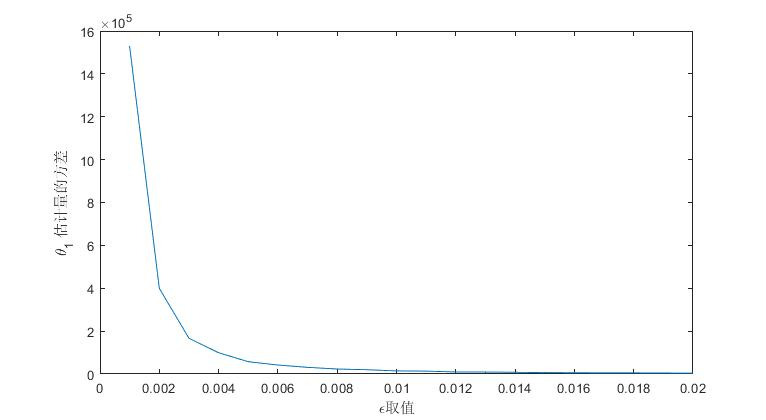
\includegraphics[scale=0.5]{fig3.1.jpg}
	\caption{\(\theta\)的第一个分量的估计量的方差随\(\epsilon\)变化曲线}
	\label{3.1}
\end{figure}

\begin{figure}[H]
	\centering
	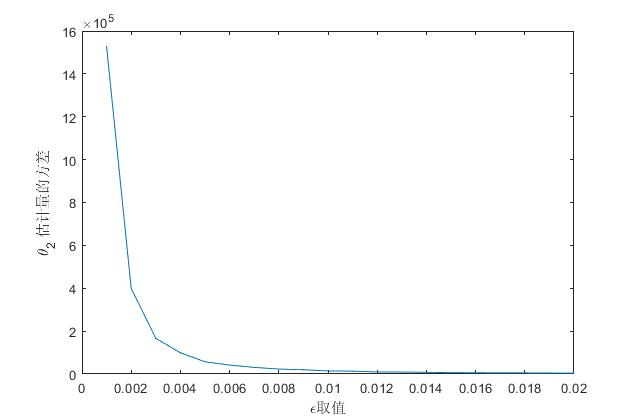
\includegraphics[scale=0.5]{fig3.2.jpg}
	\caption{\(\theta\)的第二个分量的估计量的方差随\(\epsilon\)变化曲线}
	\label{3.2}
\end{figure}

图3.1和图3.2显示了\(\theta\)的两个分量的估计量的方差随\(\epsilon\)变化曲线。从图中可以发现,随着\(\epsilon\)的减小,\(\hat{\boldsymbol{\theta}}=(\mathbf{H}^T \mathbf{H})^{-1}\mathbf{H}^T\mathbf{z}\)的估计性能逐渐变差。

\subsubsection*{*(3)如果已知\(\boldsymbol{\theta}\)中只有少部分分量非零,
	你认为选用哪种贝叶斯准则可以更好地处理该问题?为什么?}

由于\(\boldsymbol{\theta}\)中只有少部分分量非零,可以假设\(\boldsymbol{\theta}\)的各分量相互独立,
且服从均值为零的拉普拉斯分布,
即\(\boldsymbol{\theta} \sim \mathcal{L}(0,\sigma_{\theta}\mathbf{I})\),后验PDF为
\begin{align*}
	p(\boldsymbol{\theta})=\frac{1}{\sigma_{\theta}^P}
	\exp\left\{-\frac{1}{\sigma_{\theta}}\sum_{p=0}^{P-1}|\theta_p| \right\}
\end{align*}

利用\(p(\mathbf{z};\boldsymbol{\theta})\)可以得到联合概率密度函数

\begin{align*}
	p(\mathbf{z},\boldsymbol{\theta})
	 & =p(\mathbf{z}|\boldsymbol{\theta})p(\boldsymbol{\theta}) \\
	 & =\frac{1}{(2\pi \sigma_e^2)^{\frac{N}{2}}}
	\exp\left\{-\frac{1}{2\sigma_e^2} \left[\mathbf{z-H}\boldsymbol{\theta}\right]^T
	\left[\mathbf{z-H}\boldsymbol{\theta}\right]\right\}\cdot \frac{1}{\sigma_{\theta}^P}
	\exp\left\{-\frac{1}{\sigma_{\theta}}\sum_{p=0}^{P-1}|\theta_p| \right\}
\end{align*}

由上式很难求出\(p(\boldsymbol{\theta}|\mathbf{z})\)的解析形式。如果进行数值积分,后验PDF
\begin{align*}
	p(\boldsymbol{\theta}|\mathbf{z})=\frac{p(\mathbf{z}|\boldsymbol{\theta}p(\boldsymbol{\theta}))}
	{\int p(\mathbf{z|\boldsymbol{\theta}})p(\boldsymbol{\theta})d\boldsymbol{\theta}}
\end{align*}
中需要求关于\(\boldsymbol{\theta}\)的P维积分,十分困难,因此求最小均方估计存在难度。

可以使用最大后验概率准则来获得最大后验概率估计,即
\begin{align*}
	\hat{\boldsymbol{\theta}}=arg \underset{\boldsymbol{\theta}}{\max}
	p(\boldsymbol{\theta |\mathbf{z}})
\end{align*}
由于不需要计算边缘PDF,消除了积分运算,可以等价的表示为
\begin{align*}
	\hat{\boldsymbol{\theta}}=arg \underset{\boldsymbol{\theta}}{\max}p(\mathbf{z}|\boldsymbol{\theta })
	p(\boldsymbol{\theta})
\end{align*}
或
\begin{align*}
	\hat{\boldsymbol{\theta}}=arg \underset{\boldsymbol{\theta}}{\max}
	\left\{-\frac{1}{2\sigma_e^2} \left[\mathbf{z-H}\boldsymbol{\theta}\right]^T
	\left[\mathbf{z-H}\boldsymbol{\theta}\right]
	-\frac{1}{\sigma_{\theta}}\sum_{p=0}^{P-1}|\theta_p|\right\}
\end{align*}


\subsection{第四题:最小均方估计}
\subsubsection*{什么情况下可以用线性最小均方估计?}

MMSE 估计量含有多重积分的计算,在实际实践中常因其计算量太大而难以实现,
而MAP 估计量涉及多维最大值求解的问题,尽管这些问题在联合高斯的假设下容易求得,
但是在一般情况下求解不简单,因此在无法做出高斯假设的情况下,就要使用其他方法。

LMMSE 是在保留 MMSE准则的条件下,限定估计量是线性的,来确定估计量。
LMMSE 依赖于随机变量的相关性,当数据和参数相关时,可以采用LMMSE。在已知被估计量的一阶矩和二阶矩,
可以采用线性最小均方估计。

\subsubsection*{如何理解递推线性最小均方估计的几何意义?}

递推LMMSE本质是将观测矢量\(z_n\)进行正交化,产生一组彼此不相关(垂直或者正交)的随机矢量,即新息
\(z[0],z[1]-\hat{z} [1|0],z[2]-\hat{z}[2|0,1],\dots \),新息是每个新增的观测值\(z(n)\)所贡献的新的信息。
这些新息组成了LMMSE,每增加一个数据相当于产生了新息,被估计量在这个新息的投影作为修正项对估计进行更新,
从而增加了估计量的新息。

\subsubsection*{考虑如下观测模型
	\begin{align*}
		z_n=A^k+w_n,n=0,1,\dots,N-1
	\end{align*}
	其中\(A\sim \mathcal{N}(0,\sigma^2_A)\),观测噪声\(w_n\overset{i,i,d}{\sim}\mathcal{N}(0.\sigma^2)\)
	且与A相互独立。}
\subsubsection*{(1)若\(k=2,N=1\),试考虑A的线性最小均方估计并分析你的结果。}

若k=2,N=1,观测模型为\(z_0=A^2+w_0\),根据线性最小均方估计的计算公式,得
\begin{align*}
	\hat{A}=E(A)+C_{Az}C_{zz}^{-1}(z-E(z))
\end{align*}
分别计算得
\begin{align*}
	E(A)   & =0                             \\
	C_{Az} & =E[(A-E(A))(z_0-E(z))]=E[Az_0] \\
	       & =E(A(A^2+\omega_0))=E(A^3)=0   \\
	C_{zz} & =E[(z_0-E(z))(z_0-E(z))]       \\
	       & =E[z_0^2-E^2(z)-2z_0E(z)]      \\
	       & =2\sigma_A^4+\sigma^2
\end{align*}
代入得
\begin{align*}
	\hat{A}=0
\end{align*}

可见计算的A的线性最小均方估计为0,与观测数据无关,这是因为A与观测数据不是线性关系导致的.

\subsubsection*{(2)若\(k=1,N>1\),试考虑A的递推线性最小均方估计并分析其性能。}

此时观测模型变为
\begin{align*}
	z_k=A+\omega_k,n=0,1,\dots,N-1
\end{align*}
根据递推线性最小均方估计的求解过程,首先基于第一个观测量\(z[0]\)求\(\hat{A}[0]\),其中
\(\hat{A}[0]\)为A在\(z[0]\)上的投影

\begin{align*}
	\hat{A}[0]=\left( A,\frac{z_0}{|z_0|}\right)\frac{z_0}{|z_0|}=\frac{E(Az_0)}{z_0^2}z_0
	=\frac{\sigma_A^2}{\sigma_A^2+\sigma^2}z_0
\end{align*}

之后求出基于\(z[0]\)的\(z[1]\)的LMMSE估计量得到\(\hat{z}[1|0]\):
\begin{align*}
	\hat{z}[1|0]=\left( z_1,\frac{z_0}{|z_0|}\right)\frac{z_0}{|z_0|}=\frac{E(z_1 z_0)}{z_0^2}z_0
	=\frac{\sigma_A^2}{\sigma_A^2+\sigma^2}z_0
\end{align*}
之后得到新息\(z[1]-\hat{z}[1|0]\):
\begin{align*}
	\widetilde{z}_1=z[1]-\hat{z}[1|0]=z_1-\frac{\sigma_A^2}{\sigma_A^2+\sigma^2}z_0
\end{align*}
将A基于新息的LMMSE估计量\(\Delta\hat{A}[1]\)加到\(\hat{A}[0]\)上,得到\(\hat{A}[1]\):
\begin{align*}
	\Delta\hat{A}[1]=\left(A,\frac{\widetilde{z}_1}{|\widetilde{z}_1|}\right)
	\frac{\widetilde{z}_1}{|\widetilde{z}_1|}=\frac{E(A\widetilde{z}_1)}{E(\widetilde{z}_1^2)}\widetilde{z}_1
\end{align*}
令\(K[1]=\frac{E(A\widetilde{z}_1)}{E(\widetilde{z}_1^2)}\),得到
\begin{align*}
	K[1]       & =\frac{E(A\widetilde{z}_1)}{E(\widetilde{z}_1^2)}=\frac{\sigma_A^2}{2\sigma_A^2+\sigma^2} \\
	\hat{A}[1] & =\hat{A}[0]+\Delta\hat{A}[1]=\hat{A}[0]+K[1]\widetilde{z}_1
\end{align*}
根据新的观测量类推,最终结果为:
\begin{align*}
	\hat{A}[N]=\hat{A}[N-1]+\Delta\hat{A}[N]=\hat{A}[N-1]+K[N](z_n-\hat{z}[n|0,1,\dots,n-1])
\end{align*}
因为\(z[N]\)与以前的样本是不相关的,所以
\begin{align*}
	\hat{A}[N-1] & =\hat{z}[n|0,1,\dots,n-1]            \\
	\hat{A}[N]   & =\hat{A}[N-1]+K[N](z_n-\hat{A}[N-1])
\end{align*}
其中
\begin{align*}
	K[N]=\frac{Bmse(\hat{A}[N-1])}{Bmse(\hat{A}[N-1])+\sigma^2}
\end{align*}

起始值:
\begin{align*}
	\hat{A}[0]=\frac{\sigma^2_A}{\sigma^2_A+\sigma^2}z_0
\end{align*}

性能分析:
估计量的均方误差为
\begin{align*}
	Bmse(\hat{A}[N])=(1-K[N])Bmse(\hat{A}[N-1])=\frac{\sigma_A^2\sigma^2}{(N+1)\sigma^2_A+\sigma^2}
\end{align*}

可见随着估计量数目的增多,估计量的均方误差不断减小,可知非贝叶斯估计时均方误差为\(\frac{\sigma^2}{N}\),
非贝叶斯估计的均方误差始终大于贝叶斯估计的均方误差,可见由于先验信息的引入,估计精度被有效改善。

\section{检测基本理论}
\subsection{第一题:检测性能、信噪比与虚警概率}
对于高斯白噪声背景下确定信号检测问题,通过理论推导和仿真,分析检测性能与信噪比、虚警概率之间的关系。如果噪声为非高斯色噪声,试讨论:相对于高斯白噪声,非高斯、有色会试检测性能如何变化?

先考虑高斯白噪声背景下确定信号的检测问题,以\(s[n]=A\)的简单二元假设为例进行说明:
\begin{align*}
	\begin{matrix}
		\mathcal{H}_0: & z[n]=w[m]   \\
		\mathcal{H}_1: & z[n]=A+w[n]
	\end{matrix}
\end{align*}
其中\(w[m]\sim \mathcal{N}(0,\sigma^2)\),A为已知参数且A>0。判决表达式为
\begin{align*}
	\Lambda(\mathbf{z})
	=\frac{p(\mathbf{z}|\mathcal{H}_1)}{p(\mathbf{z}|\mathcal{H}_0)}
	=\frac{(2\pi \sigma^2)^{-N/2}\exp\left[-\frac{1}{2\sigma^2}\sum_{n=0}^{N-1}(z[n]-A)^2\right]}
	{(2\pi \sigma^2)^{-N/2}\exp\left[-\frac{1}{2\sigma^2}\sum_{n=0}^{N-1}(z[n])^2\right]}
	\begin{matrix}
		\mathcal{H}_1 \\>\\<\\\mathcal{H}_0
	\end{matrix}\gamma
\end{align*}
进一步化简得到:
\begin{align*}
	T(\mathbf{z})=\frac{1}{N}\sum_{n=0}^{N-1}z[n]
	\begin{matrix}
		\mathcal{H}_1 \\>\\<\\\mathcal{H}_0
	\end{matrix}
	\frac{\sigma^2}{NA}\ln \gamma+\frac{A}{2}\overset{\Delta}{=}
	\gamma^{\prime}
\end{align*}
由NP准则,检测门限由虚警概率决定:
\begin{align*}
	p_F=P\{T(\mathbf{z}>\gamma)|\mathcal{H}_0\}=Q(\frac{\gamma^{\prime}}{\sqrt{\sigma^2/N}})
\end{align*}
检测概率为
\begin{align*}
	p_D
	 & =p\{T(\mathbf{z})>\gamma|\mathcal{H}_1            \\
	 & =Q(\frac{\gamma^{\prime}-A}{\sqrt{\sigma^2/N}})\} \\
	 & =Q(Q^{-1}(P_F)-\sqrt{N}d)
\end{align*}
其中\(d=A/\sigma\)。

对于色噪声情形
\begin{align*}
	\begin{matrix}
		\mathcal{H}_0: & z[n]=w[m]      \\
		\mathcal{H}_1: & z[n]=s[n]+w[n]
	\end{matrix}
\end{align*}
其中\(\mathbf{w}\sim \mathcal{N}(\mathbf{0},\mathbf{C})\)

\begin{align*}
	p(\mathbf{z}|\mathcal{H}_1) & =\frac{1}{(2\pi )^{N/2}\det^{1/2}\mathbf{C}}
	\exp \left[-\frac{1}{2}(\mathbf{z}-\mathbf{s})^T\mathbf{C}^{-1}(\mathbf{z}-\mathbf{s})\right] \\
	p(\mathbf{z}|\mathcal{H}_0) & =\frac{1}{(2\pi )^{N/2}\det^{1/2}\mathbf{C}}
	\exp \left[-\frac{1}{2}\mathbf{z}^T\mathbf{C}^{-1}\mathbf{z}\right]                           \\
\end{align*}
判决表达式
\begin{align*}
	T(\mathbf{z})=\mathbf{z}^T\mathbf{C}^{-1}\mathbf{s}
	\begin{matrix}
		\mathcal{H}_1 \\>\\<\\\mathcal{H}_0
	\end{matrix}
\end{align*}
其中门限\(\gamma^{\prime}\)由虚警概率决定。
\begin{align*}
	E(T|\mathcal{H}_0)
	 & =E(\mathbf{w}^T\mathbf{C}^{-1}\mathbf{s})=0                        \\
	E(T|\mathcal{H}_1)
	 & =E\left[(\mathbf{s}+\mathbf{w}^T\mathbf{C}^{-1}\mathbf{s})\right]
	=\mathbf{s}^T\mathbf{C}^{-1}\mathbf{s}                                \\
	\text{var}(T|\mathcal{H}_0)
	 & =E\left[(\mathbf{w}^T\mathbf{C}^{-1}\mathbf{s})^2\right]
	=E(\mathbf{s}^T\mathbf{C}^{-1}\mathbf{ww}^T\mathbf{C}^{-1}\mathbf{s}) \\
	 & =\mathbf{s}^T\mathbf{C}^{-1}\mathbf{s}
\end{align*}
并且
\begin{align*}
	\text{var}(T|\mathcal{H}_1)
	 & =E\left[(\mathbf{z}^T\mathbf{C}^{-1}\mathbf{s}-E(\mathbf{z}^T\mathbf{C}^{-1}\mathbf{s})) \right] \\
	 & =E\left[((\mathbf{z}-E(\mathbf{z}))^T\mathbf{C}^{-1}\mathbf{s})^2\right]                         \\
	 & =E[(\mathbf{w}^T\mathbf{C}^{-1}\mathbf{s})^2]                                                    \\
	 & =\text{var}(T|\mathcal{H}_0)
\end{align*}
从而
\begin{align*}
	P_D=Q(Q^{-1}(P_{FA}-\sqrt{d^2}))=Q(Q^{-1}(P_{FA})-\sqrt{\mathbf{s}^T\mathbf{C}^{-1}\mathbf{s}})
\end{align*}

可以看出,若为色噪声,检测概率随\(\mathbf{s}^T\mathbf{C}^{-1}\mathbf{s}\)单调递增;而在高斯白噪声情况下,信号的形状是不重要的,然而现在,应设计信号使\(\mathbf{s}^T\mathbf{C}^{-1}\mathbf{s}\)最大。

对于非高斯噪声,情况较为复杂,书中已经证明了对于IID非高斯噪声中确定性信号检测问题,检测性能最差的是高斯PDF,在拉普拉斯噪声中的弱信号检测中,拉普拉斯噪声下的偏移系数大于高斯噪声,其渐进性能优于高斯噪声。

\subsection{第二题:贝叶斯准则判决式和平均代价}
考虑二元假设
\begin{align*}
	\mathcal{H}_0 & :\quad z=-1+n \\
	\mathcal{H}_1 & :\quad z=1+n
\end{align*}
其中n是均值为零,方差为1/2的高斯噪声,两种假设先验概率相等,代价因子分别为\(C_{00}=1,C_{10}=4,C_{11}=2,C_{01}=8\)
。

\subsubsection*{(1)求贝叶斯准则判决式和平均代价C1}
两种假设下的似然函数分别为
\begin{align}
	p(\mathbf{z}|\mathcal{H}_0) & =\frac{1}{\sqrt{\pi}}\exp(-(z+1)^2) \\
	p(\mathbf{z}|\mathcal{H}_1) & =\frac{1}{\sqrt{\pi}}\exp(-(z-1)^2)
\end{align}
则似然比为
\begin{align*}
	\Lambda(\mathbf{z})=\frac{p(\mathbf{z}|\mathcal{H}_1)}{p(\mathbf{z}|\mathcal{H}_0)}=\exp(4\mathbf{z})
\end{align*}
判决门限为
\begin{align*}
	\eta=\frac{(C_{10}-C_{00})q}{(C_{01}-C_{11})p}
\end{align*}
其中先验概率\(q=p\)。所以判决门限\(\eta=3/6=0.5\)。判决式\(z\begin{matrix}\mathcal{H}_1\\>\\<\\\mathcal{H_0}\end{matrix}\frac{\ln (\eta)}{4}\),即\(z\begin{matrix}\mathcal{H}_1\\>\\<\\\mathcal{H_0}\end{matrix}-0.1733\)。

下面求平均代价,先计算虚警概率
\begin{align*}
	\alpha=\int_{-0.1733}^{\infty}p(z|\mathcal{H}_0)dz=0.1212
\end{align*}
检测概率
\begin{align*}
	P_D=\int_{-0.1733}^{\infty}p(z|\mathcal{H}_1)dz=0.9515
\end{align*}
漏警概率
\begin{align*}
	\beta=\int_{-\infty}^{-0.1733}p(z|\mathcal{H}_1)dz=1-P_D=0.0485
\end{align*}
另外\begin{align*}
	P_c=\int_{-\infty}^{-0.1733}p(z|\mathcal{H}_0)dz=1-\alpha=0.8788
\end{align*}
平均代价\(C1=(C_{00}P_c+C_{10}\alpha)q+(C_{01}\beta+C_{11}P_D)p=3.6546p\)
其中\(p=q=0.5\),所以\(C1=1.8723\)。
\subsubsection*{(2)将判决门限分别增加0.002和减小0.002,分别计算平均代价C2和C3,与C1进行比较。}
当判决门限增加0.02时,\(\alpha=0.1156\),检测概率\(P_D=0.9486,P_c=1-\alpha=0.8844,\beta=1-P_D=0.0514\)
平均代价为\(C2=(C_{00}P_c+C_{10}\alpha)q+(C_{01}\beta+C_{11}P_D)=1.8276>C1\)。

当判决门限减小0.02时,\(\alpha=0.127,P_D=0.9543,P_c=1-\alpha=0.873,\beta=1-P_D=0.0457\)。
平均代价\(C3=(C_{00}P_c+C_{10}\alpha)q+(C_01\beta+C_{11}P_D)=1.8276>C1\)。

通过计算发现,贝叶斯准则门限的代价C1最小。

\subsection{第三题:NP判决式、ROC曲线与CFAR性质}
考虑二元假设
\begin{align*}
	H_0 & :z[k]=n[k]                            \\
	H_1 & :z[k]=Ar^k+n[k]\quad k=0,1,\cdots N-1
\end{align*}
噪声是服从\(n(k)\sim \mathcal{N}(0,\sigma^2)\)的WGN。

\subsubsection*{(1)若\(r(0<r<1)\)已知,且A已知,求解NP判决式。绘出当\(A=r=1\),且\(\sigma^2=1\)时,观测数据量\(N=10\)和\(N=5\)时的ROC曲线;绘出当\(A=r=1\),且\(\sigma^2=1\)时\(P_{FA}=0.01\)和\(P_{FA}=0.0001\)检测性能曲线。}

两种假设下的似然函数为:
\begin{align*}
	p(\mathbf{z}|\mathcal{H}_0) & =\frac{1}{(2\pi \sigma^2)^{N/2}}
	\exp\left[-\frac{1}{2\sigma^2}\sum_{k=0}^{N-1}z^2[k]\right]    \\
	p(\mathbf{z}|\mathcal{H}_1) & =\frac{1}{(2\pi \sigma^2)^{N/2}}
	\exp\left[-\frac{1}{2\sigma^2}\sum_{k=0}^{N-1}(z[k]-Ar^k)^2\right]
\end{align*}
判决表达式为

\begin{align*}
	\Lambda(\mathbf{z})=\frac{p(\mathbf{z}|\mathcal{H}_1)}{p(\mathbf{z|\mathcal{H}_0})}
	=\frac{(2\pi \sigma^2)^{-N/2}\exp\left[-\frac{1}{2\sigma^2}\sum_{k=0}^{N-1}(z[k]-Ar^k)^2\right]}
	{(2\pi \sigma^2)^{-N/2}\exp\left[-\frac{1}{2\sigma^2}\sum_{k=0}^{N-1}z^2[k]\right]}
	\begin{matrix}
		\mathcal{H}_1 \\>\\<\\\mathcal{H}_0
	\end{matrix}\gamma
\end{align*}
其中,门限\(\gamma\)由约束的虚警概率决定
\begin{align*}
	P_{FA}=\int_{\gamma}^{+\infty}\Lambda(\mathbf{z}|\mathcal{H}_0)d\mathbf{z}=\alpha
\end{align*}
进一步化简得到
\begin{align*}
	\exp\left[\frac{A}{\sigma^2}\sum_{i=0}^{N-1}r^kz[k]-\frac{A^2}{2\sigma^2}\frac{1-r^{2N}}{1-r^2}\right]
	\begin{matrix}
		\mathbf{H}_1 \\>\\<\\\mathcal{H}_0
	\end{matrix}\gamma
\end{align*}
即NP准则下的判决式为
\begin{align*}
	T(\mathbf{z})=\sum_{k=0}^{N-1}r^kz[k]
	\begin{matrix}
		\mathcal{H}_1 \\>\\<\\\mathcal{H}_0
	\end{matrix}
	\frac{A}{2}\frac{1-r^{2N}}{1-r^2}+\frac{\sigma^2}{A}\ln \gamma
	=\gamma^{\prime}
\end{align*}

当\(A=r=1\),且\(\sigma^2=1\)时
\begin{align*}
	P_D=Q(Q^{-1}(P_F)-\sqrt{N})
\end{align*}
虚警概率相同时,观测数据量越大,检测概率越大;观测数据量相同时,虚警概率越大,检测概率越大。

当\(A=r=1\),且\(\sigma^2=1\)时,\(P_{FA}=0.01\)和\(P_{FA}=0.00001\)时,可绘制检测概率与信噪比的关系。其中信噪比定义为功率之比,即\(d^2=NA^2/\sigma^2,P_D=Q(Q^{-1}(P_{FA}-d))\)。信噪比相同时,虚警概率越高,检测概率越高;虚警概率一定时,信噪比越高,检测概率越高。

\subsubsection*{(2)若\(r=1,A\)为随机变量,已知服从\(A\sim \mathcal{N}(\mu_A,\sigma_A^2)\)时的判决式;}

由于A为随机变量,此时为符合假设检验问题,而A的先验分布已知,因此可以选择贝叶斯方法。
首先计算似然函数
\begin{align*}
	p(\mathbf{z}|\mathcal{H}_1)
	 & =\int_{-\infty}^{\infty}p(\mathbf{z}|A,\mathcal{H}_1)p(A)dA                                 \\
	 & =\int_{-\infty}^{\infty}\frac{1}{(2\pi \sigma^2)^{N/2}}
	\exp\left[-\frac{1}{2\sigma^2}\sum_{k=0}^{N-1}(z[k]-A)^2\right]
	\cdot \frac{1}{(2\pi \sigma^2)^{1/2}}\exp\left[-\frac{1}{2\sigma^2_A}(A-\mu_A)^2\right]dA      \\
	 & =(2\pi \sigma^2)^{-N/2}(2\pi \sigma^2_A)^{-1/2}
	\int_{-\infty}^{\infty} \exp\left[-\frac{1}{2\sigma^2}\sum_{k=0}^{N-1}(z[k]-A)^2-
	\frac{1}{2\sigma^2}\sum_{k=0}^{N-1}(A-\mu_A)^2 \right]dA                                       \\
	p(\mathbf{z}|\mathcal{H}_0)
	 & =\frac{1}{(2\pi \sigma^2)^{N/2}}\exp\left(-\frac{1}{2\sigma^2}\sum_{k=0}^{N-1}z^2[k]\right)
\end{align*}
\begin{align*}
	\mathcal{Q}(A)
	 & =\frac{1}{\sigma^2}\sum_{k=0}^{N-1}(z[k]-A)^2+\frac{(A-\mu_A)^2}{\sigma^2_A}                             \\
	 & =\frac{1}{\sigma^2}\sum_{k=0}^{N-1}z^2[k]-\frac{2N}{\sigma^2}\mathbf{\overline{z}}A
	+\frac{NA^2}{\sigma^2}+\frac{(A-\mu_A)^2}{\sigma^2_A}                                                       \\
	 & =\underset{1/\sigma^2_{A|\mathbf{z}}}{\underbrace{\left(\frac{N}{\sigma^2}+\frac{1}{\sigma^2_A}\right)}}
	A^2-\frac{2A\mu_A}{\sigma^2_A}+\frac{\mu^2_A}{\sigma^2_A}-\frac{2N}{\sigma^2}\mathbf{\overline{z}}A+
	\frac{1}{\sigma^2}\sum_{k=0}^{N-1}z^2[k]                                                                    \\
	 & =\frac{1}{\sigma^2_{A|\mathbf{z}}}\left[A-
	\left(\frac{N\overline{\mathbf{z}}}{\sigma^2}+\frac{\mu_A}{\sigma_A^2}\right)\sigma^2_{A|\mathbf{z}}\right]^2
	-\left(\frac{N\overline{\mathbf{z}}}{\sigma^2}+\frac{\mu_A}{\sigma_A^2}\right)^2\sigma^2_{A|\mathbf{z}}
	+\frac{1}{\sigma^2}\sum_{k=0}^{N-1}z^2[k]+\frac{\mu^2_A}{\sigma^2_A}
\end{align*}

似然比
\begin{align*}
	\frac{p(\mathbf{z}|\mathcal{H}_1)}{p(\mathbf{z|\mathcal{H}_0})}
	 & =\frac{(2\pi \sigma^2)^{-N/2}(2\pi \sigma^2_A)^{-1/2}
	\int_{-\infty}^{\infty}\exp[-\frac{1}{2}\mathcal{Q}(A)]dA}
	{(2\pi \sigma^2)^{-N/2}\exp[-\frac{1}{2\sigma^2}\sum_{k=0}^{N-1}z^2[k]]}              \\
	 & =\frac{\sigma_{A|\mathbf{z}}}{\sigma_A}\exp\left[\frac{\sigma^2_{A|\mathbf{z}}}{2}
	\left(\frac{N\overline{\mathbf{z}}}{\sigma^2}+\frac{\mu_A}{\sigma^2_A}\right)^2-\frac{\mu^2_A}{2\sigma^2_A}\right]
	\begin{matrix}
		\mathcal{H}_1 \\>\\<\\\mathcal{H}_0
	\end{matrix}\gamma
\end{align*}
其中门限\(\gamma\)取决于判决准则,进一步换件得到最终判决表达式
\begin{align*}
	(\frac{N\overline{\mathbf{z}}}{\sigma^2}+\frac{\mu_A}{\sigma^2_A})^2
	\begin{matrix}
		\mathcal{H}_1 \\>\\<\\\mathcal{H}_0
	\end{matrix}
	\frac{2}{\sigma^2_{A|\mathbf{z}}}\ln(\frac{\sigma_A}{\sigma_{A|\mathbf{z}}})+\frac{\mu_A^2}{\sigma^2_{A|\mathbf{z}}\sigma^2_A}
	=\gamma^{\prime}
\end{align*}

\subsubsection*{(3)若\(r(0<r<1)\)已知,A未知,求解GLRT判决式,是否具有CFAR性质?}

GLRT采用最大似然估计代替未知参数A。

首先在\(\mathcal{H}_1\)假设下,求A的最大似然估计
\begin{align*}
	p(\mathbf{z}|A,\mathcal{H}_1)
	 & =(2\pi \sigma^2)^{-N/2}
	\exp\left[-\frac{1}{2\sigma^2}\sum_{k=0}^{N-1}(z[k]-Ar^k)^2\right]                   \\
	\frac{\partial \ln p(\mathbf{z}|A,\mathcal{H}_1)}{\partial A}
	 & =\frac{1}{\sigma^2}\left[\sum_{k=0}^{N-1}r^kz[k]-A\sum_{k=0}^{N-1}r^{2k}\right]=0
\end{align*}
可得A的最大似然估计为
\begin{align*}
	\hat{A}_{ml}=\frac{\sum_{k=0}^{N-1}r^kz[k]}{\sum_{k=0}^{N-1}r^{2k}}
\end{align*}
似然比为
\begin{align*}
	\Lambda_{G}(\mathbf{z})
	 & =\frac{(2\pi \sigma^2)^{-N/2}
	\exp\left\{-\frac{1}{2\sigma^2}\sum_{k=0}^{N-1}\left[z[k]-\hat{A}_{ml}r^{k}\right]^2 \right\}}
	{(2\pi \sigma^2)^{-N/2}\exp\left[-\frac{1}{2\sigma^2}\sum_{k=0}^{N-1}z^2[k] \right]}                          \\
	 & =\exp\left[-\frac{1}{2\sigma^2}\sum_{k=0}^{N-1}(\hat{A}^2_{ml}r^2k-2\hat{A}_{ml}r^kz[k])\right]            \\
	\ln \Lambda_G(\mathbf{z})
	 & =\frac{1}{2\sigma^2}\left[2\hat{A}_{ml}\sum_{k=0}^{N-1}r^kz[k]-\hat{A}^2_{ml}\sum_{k=0}^{N-1}r^{2k}\right] \\
	 & =\frac{1}{2\sigma^2}\frac{\left(\sum_{k=0}^{N-1}r^kz[k]\right)^2}{\sum_{k=0}^{N-1}r^{2k}}
	\begin{matrix}
		\mathcal{H}_1 \\>\\<\\\mathcal{H}_0
	\end{matrix}                                                                            \ln \gamma            \\
	\vert T(\mathbf{z})\vert
	 & =\vert \sum_{k=0}^{N-1}r^kz[k]\vert
	\begin{matrix}
		\mathcal{H}_1 \\>\\<\\\mathcal{H}_0
	\end{matrix}
	\sqrt{2}\sigma\sqrt{\ln \gamma\sum_{k=0}^{N-1}r^{2k}}=\gamma^{\prime}
\end{align*}
检验统计量服从高斯分布,其均值和方差为
\begin{align*}
	E[T(\mathbf{z})|\mathcal{H}_0]
	 & =E(\sum_{k=0}^{N-1}r^kn[k])=\sum_{k=0}^{N-1}r^kE(n[k])=0               \\
	\text{var}[T(\mathbf{z})|\mathcal{H}_0]
	 & =\text{var}(\sum_{k=0}^{N-1}r^kn[k])=\sigma^2\frac{1-r^{2N}}{1-r^2}    \\
	E[T(\mathbf{z})|\mathcal{H}_1]
	 & =E\left[\sum_{k=0}^{N-1}r^k(Ar^k+n[k])\right]
	=\sum_{k=0}^{N-1}r^kE(Ar^k+n[k])=A\frac{1-r^{2N}}{1-r^2}                  \\
	\text{var}\left[T(\mathbf{z})|\mathcal{H}_1\right]
	 & =\text{var}\left(\sum_{k=0}^{N-1}\sum_{k=0}^{N-1}r^k(Ar^k+n[k])\right)
	=\sigma^2\frac{1-r^{2N}}{1-r^2}
\end{align*}

\subsection{第四题:广义似然比检验、局部最大势检验与一致最大势检验}
考虑二元假设
\begin{align*}
	H_0 & :\sigma^2=\sigma^2_0 \\
	H_1 & :\sigma^2>\sigma^2_0
\end{align*}
其中观测数据样本为独立同分布,\(z[n]\sim \mathcal{N}(0,\sigma^2),\quad n=0,1,\ldots ,N-1。\)

\subsubsection*{(1)求广义似然比\(L_G(\mathbf{z})\),并证明\(L_G(\mathbf{z})\geqslant1\)恒成立。}

先求\(\mathcal{H}_1\)假设下\(\sigma^2\)的MLE:

\(\mathcal{H}_1\)假设下的似然函数为
\begin{align*}
	p(\mathbf{z}|\sigma^2_1,\mathcal{H}_1)
	 & =(2\pi \hat{\sigma}^2_1)^{-N/2}
	\exp\left[-\frac{1}{2\hat{\sigma}^2_1}\sum_{n=0}^{N-1}\right]            \\
	\frac{\partial \ln p(\mathbf{z}|\hat{\sigma}^2_1,\mathcal{H}_1)}{\partial \sigma^2_1}
	 & =-\frac{N}{2\sigma^2_1}+\frac{1}{2\sigma^4_1}\sum_{k=0}^{N-1}z^2[n]=0
\end{align*}
可以求得最大似然估计量为\(\hat{\sigma}_1^2=\sum_{n=0}^{N-1}z^2[n]/N\),广义似然比
\begin{align*}
	L_G(\mathbf{z})
	 & =\frac{p(\mathbf{z};\hat{\sigma}_1,\mathcal{H}_1)}
	{p(\mathbf{z};;\hat{\sigma}_0,\mathcal{H}_0)}                                                             \\
	 & =\frac{(2\pi \hat{\sigma}_1^2)^{(-N/2)}\exp \left\{ -\sum_{n=0}^{N-1}z^2[n]/2\hat{\sigma}_1^2\right\}}
	{(2\pi \sigma_0^2)^{(-N/2)}\exp \left\{ -\sum_{n=0}^{N-1}z^2[n]/2\sigma^2_0\right\}}                      \\
	 & =\bigg(\frac{\hat{\sigma}_1^2}{\sigma_0^2}\bigg)^{-N/2}
	\exp\left\{\frac{N}{2}(\frac{\hat{\sigma}_1^2}{\sigma_0^2}-1) \right\}
\end{align*}
而\(\hat{\sigma}_1^2=\sum_{n=0}^{N-1}z^2[n]/N\),所以
\begin{align*}
	\ln L_G(\mathbf{z})=-\frac{N}{2}\ln\frac{\hat{\sigma}_1^2}{\sigma_0^2}+\frac{N}{2}(\frac{\hat{\sigma}_1^2}{\sigma_0^2}-1)
\end{align*}
令\(\frac{\partial \ln L_G(\mathbf{z})}{\partial \hat{\sigma}_1^2}=0\),即
\begin{align*}
	\frac{\partial \ln L_G(\mathbf{z})}{\partial \hat{\sigma}_1^2}=
	-\frac{N}{2\hat{\sigma}_1^2}+\frac{N}{2\sigma_0^2}=0
\end{align*}
得到\(\hat{\sigma}_1^2=\sigma_0^2\),这时\(\frac{\partial^2 \ln L_G(\mathbf{z})}{(\partial \hat{\sigma}_1^2)^2}=\frac{N}{2(\sigma^2_1)^2}>0\),所以对数广义似然函数的最小值为\(\ln L_G(\mathbf{z})|_{\hat{\sigma}_1^2=\sigma_0^2}=0\),即\(L_G(\mathbf{z})\geqslant1\)。

\subsubsection*{(2)求广义似然比检验的检验统计量,判决准测应当采用NP准测还是最小错误概率准则(两种假设的先验概率相等),为什么?}
根据(1)中结果,广义似然比检验的检验统计量
\begin{align*}
	L_G(\mathbf{z})=\bigg(\frac{\hat{\sigma}_1^2}{\sigma_0^2}\bigg)^{-N/2}\exp\left\{\frac{N}{2}(\frac{\hat{\sigma}_1^2}{\sigma_0^2}-1) \right\}>\gamma
\end{align*}
则GLRT判\(\mathcal{H}_1\),等价于
\begin{align*}
	\ln L_G(\mathbf{z})=-\frac{N}{2}\ln\frac{\hat{\sigma}_1^2}{\sigma_0^2}+\frac{N}{2}(\frac{\hat{\sigma}_1^2}{\sigma_0^2}-1)>\ln \gamma
\end{align*}

由于门限与\(\sigma^2_1\)有关,不满足选取\(\gamma\)满足虚警概率\(\alpha\)为常数的约束条件,所以不能用NP准测。这时可以考虑用最小错误概率准测,对\(\sigma^2_1\)指定先验PDF。
\subsubsection*{(3)求局部最大势(LMP)检验,分析检验统计量与充分统计量的关系}
局部最大势检验的检验统计量为
\begin{align*}
	T_{LMP}(\mathbf{z})=\frac{\frac{\partial \ln p(\mathbf{z;\sigma^2})}{\partial \sigma^2}|_{\sigma^2=\sigma^2_0}}{\sqrt{I(\sigma^2_0)}}
\end{align*}
而
\begin{align*}
	\frac{\partial \ln p(\mathbf{z;\sigma^2})}{\partial \sigma^2}
	 & =\frac{\partial }{\partial \sigma^2}\ln \left\{(2\pi \sigma^2)^{-N/2}\exp\left[ -\frac{\sum_{n=0}^{N-1}z^2[n]}{2\sigma^2}\right]\right\} \\
	 & =\frac{\partial }{\partial \sigma^2}\left[-\frac{N}{2} \ln(2\pi \sigma^2)-\frac{\sum_{n=0}^{N-1}z^2[n]}{2\sigma^2}\right]                \\
	 & =\frac{\sum_{n=0}^{N-1}z^2[n]}{2(\sigma^2)^2}-\frac{N}{2 \sigma^2}                                                                       \\
	 & =\frac{\sum_{n=0}^{N-1}z^2[n]-N\sigma^2 }{2 (\sigma^2)^2}
\end{align*}
Fisher信息
\begin{align*}
	I(\sigma_0^2)
	 & =-E\left[ \frac{\partial^2 \ln p(\mathbf{z;\sigma^2})}{(\partial \sigma^2)^2}\right]|_{\sigma^2=\sigma^2_0}  \\
	 & =-E\left[ \frac{N}{2 (\sigma^2)^2}-\frac{\sum_{n=0}^{N-1}z^2[n]}{(\sigma^2)^3}\right]|_{\sigma^2=\sigma^2_0} \\
	 & =\frac{N}{2 (\sigma^2_0)^2}
\end{align*}
所以
\begin{align*}
	T_{LMP}(\mathbf{z})
	 & =\frac{\sum_{n=0}^{N-1}z^2[n]-N\sigma^2 }{2 (\sigma^2)^2}\cdot\frac{\sqrt{2}\sigma_0^2}{\sqrt{N}} \\
	 & =\frac{\sqrt{N}}{\sqrt{2}\sigma^2_0}(\frac{1}{N}\sum_{n=0}^{N-1}z^2[n]-\sigma^2_0)                \\
	 & =\frac{\sqrt{N}}{\sqrt{2}\sigma^2_0}(\hat{\sigma}^2-\sigma^2_0)
\end{align*}

根据Neyman-Fisher因子分解定理,
\begin{align*}
	p(\mathbf{z};\sigma^2)
	 & =\frac{1}{(2\pi \sigma^2)^{N/2}}\exp\left\{ -\frac{\sum_{n=0}^{N-1}z^2[n]}{2\sigma^2}\right\}        \\
	 & =\frac{1}{(2\pi \sigma^2)^{N/2}}\exp\left\{ -\frac{\sum_{n=0}^{N-1}z^2[n]}{2\sigma^2}\right\}\cdot 1 \\
	 & =g(T(\mathbf{z},\sigma^2))\cdot h(\mathbf{z})
\end{align*}
充分统计量为
\begin{align*}
	T(\mathbf{z})=\sum_{n=0}^{N-1}z^2[n]
\end{align*}
所以检验统计量
\begin{align*}
	T_{LMP}(\mathbf{z})=\frac{\sqrt{N}}{\sqrt{2}\sigma^2_0}(\frac{1}{N}T(\mathbf{z})-\sigma^2_0)
\end{align*}
是充分统计量的函数。这时因为充分统计量包含了在数据中做出判决所需要的关于方差的所有信息。
\subsubsection*{(4)存在一致最大势检验吗?}
考虑一致最大势检验:
\begin{align*}
	\Lambda(\mathbf{z})
	 & =\frac{p(\mathbf{z;\sigma^2_1,\mathcal{H}_1})}{p(\mathbf{z;\mathcal{H}_0})}                            \\
	 & =\frac{(2\pi \hat{\sigma}_1^2)^{(-N/2)}\exp \left\{ -\sum_{n=0}^{N-1}z^2[n]/2\hat{\sigma}_1^2\right\}}
	{(2\pi \sigma_0^2)^{(-N/2)}
	\exp \left\{ -\sum_{n=0}^{N-1}z^2[n]/2\sigma^2_0\right\}}                                                 \\
	 & =\bigg(\frac{\sigma_1^2}{\sigma_0^2}\bigg)^{-N/2}
	\exp \left\{\frac{\sum_{n=0}^{N-1}z^2[n]}{2}(\sigma_0^{-2}-\sigma_1^{-2}) \right\}                        \\
	 & >\gamma
\end{align*}
两边取对数得到
\begin{align*}
	-\frac{N}{2}\ln\bigg(\frac{\sigma_1^2}{\sigma_0^2}\bigg)+
	\frac{\sum_{n=0}^{N-1}z^2[n]}{2}(\sigma_0^{-2}-\sigma_1^{-2})>\ln\gamma
\end{align*}

由于\(\sigma_1^2>\sigma_1^2\),所以\(\sigma_0^{-2}-\sigma_1^{-2}>0\),整理得到
\begin{align*}
	\frac{1}{N}\sum_{n=0}^{N-1}z^2[n]>\left[\frac{2}{N}\ln\gamma+\ln\bigg(\frac{\sigma_1^2}{\sigma_0^2}\bigg)\right](\sigma_0^{-2}-\sigma_1^{-2})^{-1}=\gamma^{\prime}
\end{align*}
检验统计量刚好是方差的估计。

参考例5.1和例6.1。在\(\mathcal{H}_0\)条件下,\(T(\mathbf{z})=\frac{1}{N}\sum_{n=0}^{N-1}z^2[n]\sim \mathcal{N}(0,\sigma^2/N)\),具有确定的分布,\(P_{FA}=Q(\frac{N\gamma^{\prime}}{\sigma_0^2})\),所以\(\gamma^{\prime}=\frac{\sigma^2_0}{N}Q^{-1}(P_{FA})\)与\(\sigma_1^2\)无关。由于在\(\mathcal{H}_0\)条件下,\(T(\mathbf{z})\)的PDF与\(\sigma_1^2\)无关,根据给定的虚警,可以计算出门限值,它是与\(\sigma_1^2\)无关的。那么给定的虚警概率\(P_{FA}\)时,对于任意的\(\sigma_1^2\),如果\(T(\mathbf{z}>\gamma^{\prime})\)则判别\(\mathcal{H}_1\)的检测器具有最高的\(P_D\),所以存在一致最大势检验。

\section{确定性信号检测}
\subsection{第一题:雷达线性调频信号的匹配滤波器}
假设雷达发射信号为线性调频信号\(u(n)=e^{j\pi \mu (nT)^2},|nT_s|\leqslant\frac{T}{2}\),其中\(T\)为脉冲宽度,\(T_s\)为采样间隔,\(\mu=\frac{B}{T}\)为调制斜率,\(B\)为信号带宽。目标距离为\(R\),目标回波幅度为\(A\),雷达接收信号表示为\(z(n)=Au(n-n_0)+w(n),n_0=\frac{2R}{cT_s},w(n)\)服从均值为0,方差为\(\sigma^2\)的高斯白噪声。

1、设\(T=0.1ms,T_s=1.25\times 10^{-7},B=4MHz\)。试设计匹配滤波器,求匹配滤波后目标输出信号表达式,并进行仿真分析。

匹配滤波器的时域表达式为
\begin{align*}
	h(n)=u^*(-n)=e^{-j[\pi \mu (nT_s)^2]}\quad |nT_s|<\frac{T}{2}
\end{align*}
匹配滤波输出结果为
\begin{align*}
	y(n)=h(n)*z(n)=AT\sin\left[c\mu T(n-n_0)\right]+w(n)*h(n)
\end{align*}
匹配滤波前目标混在噪声中,无法提取秒信号;在匹配滤波后。目标回波被压缩在\(t=20\mu s\)处,与真实位置\(R=3000m\)吻合。

2、如果存在认为干扰信号,干扰信号形式为\(u_j(n)=A_Je^{}j2\pi f_{JK}\cdot nT_S+j\pi \mu(nT_s)^2,|nT_s|\leqslant\frac{T}{2},f_{JK}=f_{J0}+(k-1)\Delta f_J,\quad k=1,2,3,\cdots,K,f_{J0}=0.5MHz,\Delta f_J=0.4MHz\)。试分析不同\(A_J\)、\(K\)下雷达匹配滤波后的输出信号。

首先对干扰信号进行分析
\begin{align*}
	u_j(n)
	 & =A_J\exp\left[j2\pi f_{jk}nT_s+j\pi \mu (nT_s)^2\right]                                    \\
	 & =A_J\exp\left[j\pi (\mu nT_s+f_{JK}/\mu)^2\right]\cdot \exp\left[-j\pi f_{jk}^2/\mu\right] \\
	 & =A_J^{\prime}\exp\left[j\pi (\mu nT_s+f_{JK}/\mu)^2\right]
\end{align*}
此时接收信号的形式为
\begin{align*}
	z(n)=Au(n-n_0)+u_j(n)+w(n)
\end{align*}
匹配滤波输出结果为
\begin{align*}
	y(n)
	 & =h(n)*z(n)                                                                               \\
	 & =AT\sin\left[c\mu T(n-n_0)+A_J^{\prime}\sin \left[c\mu T (n+n_c)\right]+w(n)*h(n)\right]
\end{align*}
其中\(n_c=f_{JK}/(\mu T_s)\)。可以看出,受干扰的信号会在\(t=-f_{JK}/\mu\)处存在干扰尖峰。

\subsection{第二题:雷达信号"M/N"检测问题。}

对于“\(M/N\)”检测,即\(N\)次独立检测,\(M\)次检测到目标即确定目标存在(虚警类似)。

考虑二元假设
\begin{align*}
	\begin{matrix}
		H_0: & z(k)=n(k)   \\
		H_1: & z(k)=A+n(k)
	\end{matrix}\quad k=0,1,\cdots N-1
\end{align*}
其中噪声\(n(k)\)是服从参量\(\sigma^2\)已知的瑞利分布。

1、对于单个观测数据作为检验统计量,分析检测门限和检测概率;

2、对于N个观测数据进行独立检测,采用“\(1/N\)”检测,分析检测概率及虚警概率。假定单次虚警概率设定为\(0.01,\sigma^2=1,A=1,N=10\),进行仿真分析;

3、若采用“\(2/4\)”检测,要求总体检测概率达到\(0.99\),分析单次检测概率要求,分析虚警概率和单次虚警概率关系。

\subsubsection*{(1)对于单个观测数据作为检验统计量,分析检测门限和检测概率.}

对于单个观测数据,可以求得NP检验:
\begin{align*}
	L(\mathbf{\mathbf{z}})=\frac{p(\mathbf{x};\mathcal{H}_1)}{p(\mathbf{x};\mathcal{H}_0)}
	=\frac{(z-A)\sigma^{-2}\exp\left[-(z-A)^2\sigma^{-2}\right]}
	{z\sigma^{-2}\exp\left[-z^2\sigma^{-2}\right]}>\gamma
\end{align*}

或者
\begin{align*}
	(1-\frac{A}{z})\exp[\sigma^{-2}(2zA-A^2)]>\gamma
\end{align*}
则判\(\mathcal{H}_1\)。
其中门限\(\gamma\)由
\begin{align*}
	P_{FA}=\int_{\{\mathbf{z}:L(\mathbf{z}>\gamma)\}}p(\mathbf{z};\mathcal{H}_0)d\mathbf{x}
\end{align*}
求出。

将单个观测数据作为检验统计量,即\(T(\mathbf{z})=z\)对于瑞利分布,虚警概率
\begin{align*}
	P_{FA} & =P\{z[0]>\gamma;\mathcal{H}_0\}                                                     \\
	       & =\int_{\gamma}^{\infty}p(z[0];\mathcal{H}_0)dz                                      \\
	       & =\int_{\gamma}^{\infty}\frac{z}{\sigma^2}\exp \left(-\frac{z^2}{2\sigma^2}\right)dz \\
	       & =\exp\left(-\frac{-\gamma^2}{\sigma^2}\right)
\end{align*}

所以检测门限\(\gamma\)为:
\begin{align*}
	\gamma=\sqrt{(-2\sigma^2)\ln P_{FA}}
\end{align*}

检测概率
\begin{align*}
	P_D & =P\{T(\mathbf{z})>\gamma;\mathcal{H}_1\}                                                  \\
	    & =\int_{\gamma}^{\infty}p(z;\mathcal{H}_1)dz                                               \\
	    & =\int_{\gamma}^{\infty}\frac{(z-A)}{\sigma^2}\exp\left[-\frac{(z-A)^2}{\sigma^2}\right]dz \\
	    & =\exp\left(-\frac{(\gamma-A)^2}{2\sigma^2}\right)                                         \\
	    & =\exp\left(-\frac{(\sqrt{(-2\sigma^2)\ln P_{FA}}-A)^2}{2\sigma^2}\right)
\end{align*}

随着虚警概率\(P_{FA}\)的增大,检测门限\(\gamma\)逐渐减小。通常虚警概率\(P_{FA}\)很小,\(\sqrt{(-2\sigma^2)\ln P_{FA}}<A\)检测概率\(P_D\)随虚警概率\(P_{FA}\)的增大而增大。

\subsubsection*{(2)对于N个观测数据进行独立检测,采用“\(1/N\)”检测,分析检测概率及虚警概率。假定单次虚警概率设定为\(0.01,\sigma^2=1,A=1,N=10\),进行仿真分析.}

对于N个观测数据进行独立检测,检测到1次即判\(\mathcal{H}_1\)。

单次观测的虚警概率为\(P(\mathcal{H}_1;\mathcal{H}_0)=P_{FA}\),\(P(\mathcal{H}_0;\mathcal{H}_0)=1-P_{FA}\),对于“\(1/N\)”检测,事件\(\{\mathcal{H}_0;\mathcal{H}_0\}_{1/N}\)需要连续N次单个观测都出现\(\{\mathcal{H}_0;\mathcal{H}_0\}\),即\(P^{1/N}\{\mathcal{H}_0;\mathcal{H}_0\}=[P(\mathcal{H}_0;\mathcal{H}_0)]^N=(1-P_{FA})^N\),所以“\(1/N\)”检测的虚警概率
\begin{align*}
	P^{1/N}_{FA} & =P^{1/N}(\mathcal{H}_1;\mathcal{H}_0)     \\
	             & =1-P^{1/N}\{\mathcal{H}_0;\mathcal{H}_0\} \\
	             & =1-(1-P_{FA})^N
\end{align*}

同理,单次观测的检测概率为\(P(\mathcal{H}_1;\mathcal{H}_1)=P_D\),漏警概率\(P(\mathcal{H}_0;\mathcal{H}_1)=1-P_D\),对于“\(1/N\)”检测,漏警\(\{\mathcal{H}_0;\mathcal{H}_1\}_{1/N}\)需要连续N次单个观测都出现漏警\(\{\mathcal{H}_0;\mathcal{H}_1\}\),即\(P^{1/N}\{\mathcal{H}_0;\mathcal{H}_1\}=[P(\mathcal{H}_0;\mathcal{H}_1)]^N=(1-P_D)^N\),所以“\(1/N\)”检测的检测概率
\begin{align*}
	P^{1/N}_D & =P^{1/N}(\mathcal{H}_1;\mathcal{H}_1)     \\
	          & =1-P^{1/N}\{\mathcal{H}_0;\mathcal{H}_1\} \\
	          & =1-(1-P_D)^N
\end{align*}

根据第\(\mathbf{(1)}\)问可知
\begin{align*}
	P_D =\exp\left(-\frac{(\sqrt{(-2\sigma^2)\ln P_{FA}}-A)^2}{2\sigma^2}\right)
\end{align*}
所以“\(1/N\)”检测的检测概率为
\begin{align*}
	P^{1/N}_D=1-\left(1-\exp\left(-\frac{(\sqrt{(-2\sigma^2)\ln P_{FA}}-A)^2}{2\sigma^2}\right)\right)^N
\end{align*}

假定单次虚警概率设定为\(0.01,\sigma^2=1,A=1,N=10\),可以计算得到
检测门限为
\begin{align*}
	\gamma & =\sqrt{(-2\sigma^2)\ln P_{FA}} \\
	       & =\gamma=\sqrt{-2\ln 0.01}      \\
	       & =3.0349
\end{align*}

虚警概率为
\begin{align*}
	P^{1/N}_{FA} & =1-(1-P_{FA})^N  \\
	             & =1-(1-0.01)^{10} \\
	             & =0.0956
\end{align*}

检测概率为
\begin{align*}
	P^{1/N}_D & =1-\left(1-\exp\left(-\frac{(\sqrt{(-2\sigma^2)\ln P_{FA}}-A)^2}{2\sigma^2}\right)\right)^N \\
	          & =1-\left(1-\exp\left(-\frac{(\sqrt{(-2)\ln 0.01}-1)^2}{2}\right)\right)^N                   \\
	          & =0.7403
\end{align*}

\begin{figure}[H]
	\centering
	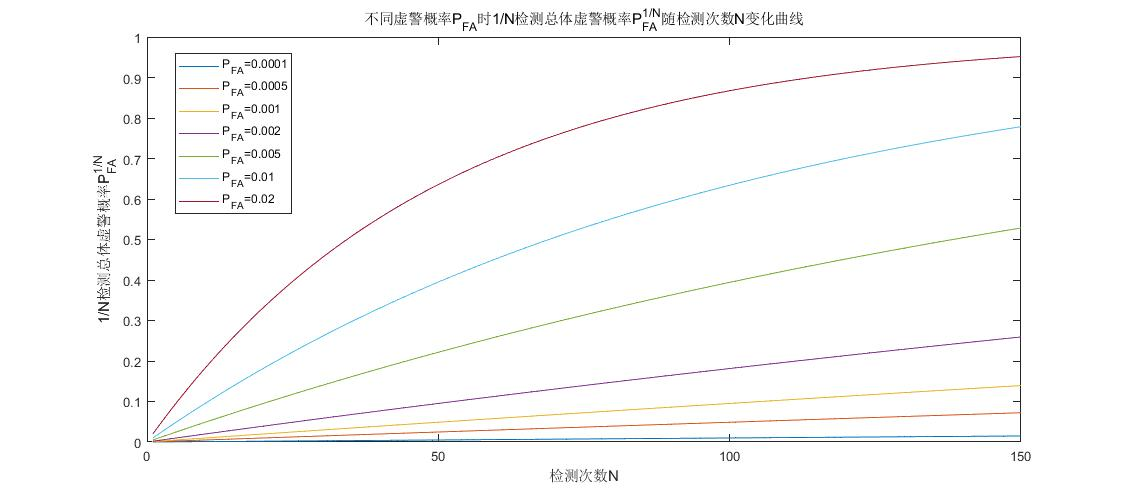
\includegraphics[scale=0.35]{fig2_1.jpg}
	\caption{不同虚警概率\(P_{FA}\)时1/N检测总体虚警概率\(P^{1/N}_{FA}\)随检测次数N变化曲线}
	\label{5.2.1}
\end{figure}

\begin{figure}[H]
	\centering
	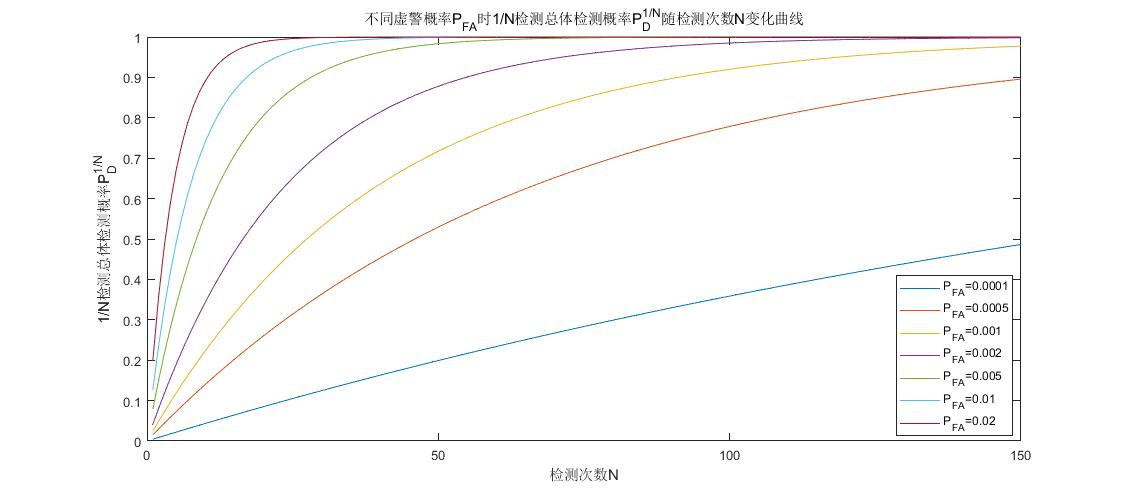
\includegraphics[scale=0.35]{fig2_2.jpg}
	\caption{不同虚警概率\(P_{FA}\)时1/N检测总体检测概率\(P^{1/N}_D\)随检测次数N变化曲线}
	\label{5.2.2}
\end{figure}

令\(\sigma^2=1,A=1\),当\(P_FA\)等于\(1\times10^{-5},5\times10^{-5},1\times10^{-4},1\times10^{-3},2\times10^{-3},5\times10^{-3},1\times10^{-2},2\times10^{-2}\)时,分别计算总体虚警概率\(P^{1/N}_{FA}\)和总体检测概率\(P^{1/N}_D\)随检测次数N的变化曲线。
得到结果如图\ref*{5.2.1}和图\ref*{5.2.2}

对比图\ref*{5.2.1}和图\ref*{5.2.2}可以发现,当单次虚警概率\(P_{FA}<0.001\)时,总体虚警概率\(P^{1/N}_{FA}\)随检测次数N增长变化不大,而总体检测概率随检测次数N增长逐渐增加到1。当增加单次虚警概率到\(0.02\)时,虽然总体检测概率在检测次数\(N=20\)时就快速增加到1,但是总体虚警概率\(P^{1/N}_{FA}\)增加也十分快速,\(N=20\)时约为0.34,\(N=100\)时约为0.87,\(N=150\)时约为0.95。所以综合考虑总体虚警概率和总体检测概率,单次虚警概率应当设置为\(P_{FA}=0.001\),检测次数N应当设置在50与100之间,这时总体虚警概率不超过0.1,检测概率在0.7至0.9之间。

\subsubsection*{(3)若采用“\(2/4\)”检测,要求总体检测概率达到\(0.99\),分析单次检测概率要求,分析虚警概率和单次虚警概率关系}

若采用“\(2/4\)”检测,类似第\(\mathbf{(2)}\)问中分析,检测概率
\begin{align*}
	P^{2/4}_D & =1-(1-P_D)^4-C_4^1P_D(1-P_D)^3 \\
	          & =1-(1-P_D)^4-4P_D(1-P_D)^3     \\
	          & \geqslant0.99
\end{align*}
解得\(P_D\geqslant 0.8591\),所以单次检测概率的取值范围为\([0.8591,1]\)。

虚警概率\(P^{2/4}_{FA}\)和单次虚警概率\(P_{FA}\)的关系为
\begin{align*}
	P^{2/4}_{FA} & =1-(1-P_{FA})^4-C_4^1P_{FA}(1-P_{FA})^3 \\
	             & =3P_{FA}^4-8P_{FA}^3+6P_{FA}^2
\end{align*}

图\ref*{5.2.3}画出了虚警概率\(P^{2/4}_{FA}\)随单次虚警概率\(P_{FA}\)变化曲线,并画出了\(6P_{FA}^2\)的变化曲线作为变化趋势的参考。
\begin{figure}[H]
	\centering
	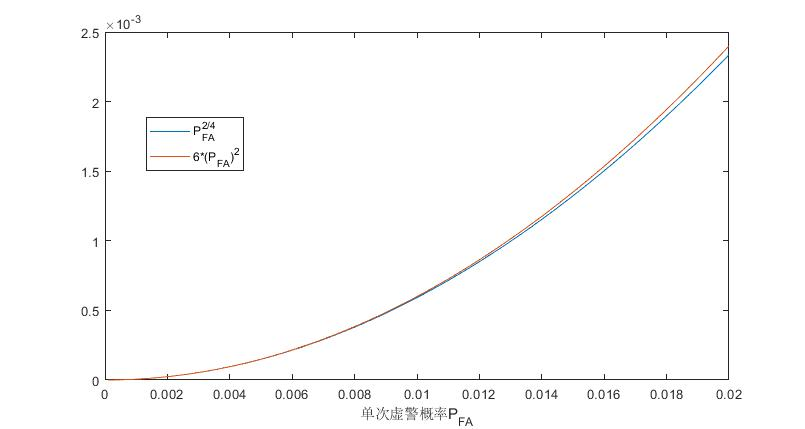
\includegraphics[scale=0.5]{fig2_3.jpg}
	\caption{总体虚警概率\(P^{2/4}_{FA}\)变化趋势比较图}
	\label{5.2.3}
\end{figure}

\subsection{第三题:高斯白噪声与色噪声下检测门限与检测概率}

高斯噪声中已知信号的分析与仿真,考虑二元假设
\begin{align*}
	\begin{matrix}
		H_0: & z(k)=n(k)     \\
		H_1: & z(k)=r^k+n(k)
	\end{matrix}\quad k=0,1,\cdots N-1
\end{align*}

1、噪声是服从\(n(k)\sim \mathcal{N}(0,1)\)的WGN,若\(r=0.9,N=20\),虚警概率设定为0.01,分析检测门限及检测概率并仿真;

2、噪声服从\(\mathcal{N}(0,\mathbf{C}),[\mathbf{C}]_{ij}=c[i-j]\),其中\(c[k]=\frac{0.19}{1-0.9^2}0.9^{|k|}\),若\(r=0.9,N=20\),虚警概率设定为\(0.01\),分析检测门限及检测概率并仿真。

\subsubsection*{(1)噪声是服从\(n(k)\sim \mathcal{N}(0,1)\)的WGN,若\(r=0.9,N=20\),虚警概率设定为0.01,分析检测门限及检测概率并仿真.}

利用NP准则,采用判决式
\begin{align*}
	L(\mathbf{z})=\frac{p(\mathbf{z};\mathcal{H}_0)}{p(\mathbf{z};\mathcal{H}_1)}>\gamma
\end{align*}
则判\(\mathcal{H}_1\)
其中
\begin{align*}
	p(\mathbf{z};\mathcal{H}_0)
	 & =\frac{1}{(2\pi\sigma^2)^{N/2}}\exp\left\{-\frac{1}{2\sigma^2}\sum_{k=0}^{N-1}z^2[k]\right\}       \\
	p(\mathbf{z};\mathcal{H}_1)
	 & =\frac{1}{(2\pi\sigma^2)^{N/2}}\exp\left\{-\frac{1}{2\sigma^2}\sum_{k=0}^{N-1}(z[k]-r^k)^2\right\} \\
\end{align*}

由此可得
\begin{align*}
	L(\mathbf{z})=\exp\left\{-\frac{1}{2\sigma^2}(-2)\sum_{k=0}^{N-1}r^k(z[k]+\frac{1-r^{2N}}{1-r^2})\right\}>\gamma
\end{align*}
两边取对数
\begin{align*}
	\ln L(\mathbf{z})=\frac{1}{\sigma^2}\sum_{k=0}^{N-1}z[k]r^k-\frac{1}{2\sigma^2}+\frac{1-r^{2N}}{1-r^2}>\ln\gamma
\end{align*}
整理得到
\begin{align*}
	\sum_{k=0}^{N-1}r^kz[k]>\sigma^2 \ln \gamma+\frac{1-r^{2N}}{2(1-r^2)}=\gamma^{\prime}
\end{align*}

令左边为检验统计量\(T(\mathbf{z})\),每种假设下的均值和方差分别为
\begin{align*}
	E[T(\mathbf{z});\mathcal{H}_0]   & =E\left[\sum_{k=0}^{N-1}r^kn(k)\right]=\sum_{k=0}^{N-1}r^kE[n(k)]=0                                \\
	E[T(\mathbf{z};\mathcal{H}_1)]   & =E\left[\sum_{k=0}^{N-1}r^k(r^k+n(k))\right]=\sum_{k=0}^{N-1}r^kE[r^k+n(k)]=\frac{1-r^{2N}}{1-r^2} \\
	Var[T(\mathbf{z});\mathcal{H}_0] & =Var\left(\sum_{k=0}^{N-1}r^kn(k)\right)=\sigma^2\frac{1-r^{2N}}{1-r^2}                            \\
	Var[T(\mathbf{z});\mathcal{H}_0] & =Var\left(\sum_{k=0}^{N-1}r^k(r^k+n(k))\right)=\sigma^2\frac{1-r^{2N}}{1-r^2}
\end{align*}

所以有
\begin{align*}
	T(\mathbf{z})\sim\left\{
	\begin{matrix}
		\mathcal{N}(0,\sigma^2\frac{1-r^{2N}}{1-r^2}),                      & \mathcal{H}_0 \\
		\mathcal{N}(\frac{1-r^{2N}}{1-r^2},\sigma^2\frac{1-r^{2N}}{1-r^2}), & \mathcal{H}_1
	\end{matrix}
	\right.
\end{align*}
可以求得
\begin{align*}
	P_{FA} & =Pr\{T(\mathbf{z})>\gamma^{\prime};\mathcal{H}_0\}=Q\left\{\frac{\gamma^{\prime}\sqrt{1-r^2}}{\sqrt{\sigma^2(1-r^{2N})}}\right\}                                                               \\
	P_D    & =Pr\{T(\mathbf{z})>\gamma^{\prime};\mathcal{H}_1\}=Q\left\{\frac{\gamma^{\prime}\sqrt{1-r^2}}{\sqrt{\sigma^2(1-r^{2N})}}-\frac{\gamma^{\prime}\sqrt{1-r^{2N}}}{\sqrt{\sigma^2(1-r^2)}}\right\}
\end{align*}
由虚警概率可以求得门限
\begin{align*}
	\gamma^{\prime}=\sqrt{\sigma^2\frac{1-r^{2N}}{1-r^2}}Q^{-1}(P_{FA})
\end{align*}
代入\(r=0.9,N=20,P_{FA}=0.01\),可得\(\gamma^{\prime}=5.2973,P_D=0.4804\)。

用MATLAB进行蒙特卡洛仿真,信号长度为20,仿真次数为10000次,仿真得到的阈值和检测概率分布为\(\gamma^{\prime}=5.2974,P_D=0.4831\),与理论值基本一致。

\subsubsection*{(2)噪声服从\(\mathcal{N}(0,\mathbf{C}),[\mathbf{C}]_{ij}=c[i-j]\),其中\(c[k]=\frac{0.19}{1-0.9^2}0.9^{|k|}\),若\(r=0.9,N=20\),虚警概率设定为\(0.01\),分析检测门限及检测概率并仿真}

噪声协方差矩阵为
\begin{align*}
	\mathbf{C}=
	\begin{bmatrix}
		1         & 0.9       & 0.9^2     & \cdots & 0.9^{N-1} \\
		0.9       & 1         & 0.9       & \cdots & 0.9^{N-2} \\
		0.9^2     & 0.9       & 1         & \cdots & 0.9^{N-3} \\
		\vdots    & \vdots    & \vdots    & \ddots & \vdots    \\
		0.9^{N-1} & 0.9^{N-2} & 0.9^{N-3} & \cdots & 1
	\end{bmatrix}
\end{align*}
利用广义匹配滤波器进行检测,检测器可以表示为:
\begin{align*}
	T(\mathbf{z})=\mathbf{z}^T\mathbf{C}^{-1}\mathbf{s}<\ln \gamma+\frac{1}{2}\mathbf{s}^T\mathbf{C}^{-1}\mathbf{s}=\gamma^{\prime}
\end{align*}
其中\(s(k)=r^k\),检验统计量满足
\begin{align*}
	T(\mathbf{z})\sim\left\{
	\begin{matrix}
		\mathcal{N}(0,\mathbf{s}^T\mathbf{C}^{-1}\mathbf{s}),                                     & \mathcal{H}_0 \\
		\mathcal{N}(\mathbf{s}^T\mathbf{C}^{-1}\mathbf{s},\mathbf{s}^T\mathbf{C}^{-1}\mathbf{s}), & \mathcal{H}_1
	\end{matrix}
	\right.
\end{align*}
可以求得:
\begin{align*}
	P_{FA} & =Pr\{T(\mathbf{z})>\gamma^{\prime};\mathcal{H}_0\}=Q\left\{\frac{\gamma^{\prime}}{\sqrt{\mathbf{s}^T\mathbf{C}^{-1}\mathbf{s}}}\right\}                                              \\
	P_D    & =Pr\{T(\mathbf{z})>\gamma^{\prime};\mathcal{H}_1\}=Q\left\{\frac{\gamma^{\prime}}{\sqrt{\mathbf{s}^T\mathbf{C}^{-1}\mathbf{s}}}-\sqrt{\mathbf{s}^T\mathbf{C}^{-1}\mathbf{s}}\right\}
\end{align*}
可以求得门限
\begin{align*}
	\gamma^{\prime}=\sqrt{\mathbf{s}^T\mathbf{C}^{-1}\mathbf{s}}Q^{-1}(P_FA)
\end{align*}
此时检测概率
\begin{align*}
	P_D=Q(Q^{-1}(P_{FA})-\sqrt{\mathbf{s}^T\mathbf{C}^{-1}\mathbf{s}})
\end{align*}
计算可得\(\mathbf{s}^T\mathbf{C}^{-1}\mathbf{s}=1\),代入数值得:\(\gamma^{\prime}=2.3263,P_D=0.0924\)。

用MATLAB进行蒙特卡洛仿真,信号长度为20,仿真次数为10000次,仿真得到的阈值和检测概率分布为\(\gamma^{\prime}=2.3263,P_D=0.0951\),与理论值基本一致。

\subsection{第四题:部分参数未知的正弦信号检测}

高斯噪声中正弦信号的分析与仿真:考虑二元假设
\begin{align*}
	\begin{matrix}
		H_0: & z(k)=n(k)                        \\
		H_1: & z(k)=A\cos(2\pi f_0 k+\phi)+n(k)
	\end{matrix}\quad k=0,1,\cdots N-1
\end{align*}
噪声是服从\(n(k)\sim \mathcal{N}(0,\sigma^2)\)的WGN,\(\sigma^2\)已知的瑞利分布。

1、若频率\(f_0\)已知,幅度和相位\(A,\phi\)未知(假定\(A>0\)),若\(\sigma^2=1,f_0=0.1,N=20\),虚警概率设定为\(0.01\),分析检测门限及检测概率并仿真;

2、若频率\(f_0\)及幅度相位\(A,\phi \)均未知(假定\(0<f_0<1/2,A>0\)),若\(\sigma^2=1,N=20\),虚警概率设定为\(0.01\),分析检测门限及检测概率并仿真。

\subsubsection*{(1)若频率\(f_0\)已知,幅度和相位\(A,\phi\)未知(假定\(A>0\)),若\(\sigma^2=1,f_0=0.1,N=20\),虚警概率设定为\(0.01\),分析检测门限及检测概率并仿真.}

可以求得幅度\(A\)和相位\(\phi\):
\begin{align*}
	\hat{A}_{MLE}    & =\sqrt{\alpha_1+\alpha_2}            \\
	\hat{\phi}_{MLE} & =\arctan(-\frac{\alpha_2}{\alpha_!})
\end{align*}
其中\(\alpha_1=\frac{2}{N}\sum_{k=0}^{N-1}z[k]\cos 2\pi f_0 k,\alpha_2=\frac{2}{N}\sum_{k=0}^{N-1}z[k]\sin 2\pi f_0 k\),

似然比与判决门限之间的关系为
\begin{align*}
	\Lambda(\mathbf{z})
	 & =\frac{p(\mathbf{z}|\hat{A}_{MLE},\hat{\phi}_{MLE},\mathcal{H}_1)}{p(\mathbf{z}|\mathcal{H}_0)}                                                                                                                                    \\
	 & =\frac{(2\pi \sigma^2)^{-N/2}\exp\left\{-2\sigma^{-1}\sum_{k=0}^{N-1}\left[z(k)-\hat{A}_{MLE}\cos(2\pi f_0k+\hat{\phi}_{MLE})\right]^2 \right\}}{(2\pi \sigma^2)^{-N/2}\exp\left\{-(2\sigma)^{-1} \sum_{k=0}^{N-1}z^2(k) \right\}}
	\begin{matrix}
		\mathcal{H}_1 \\>\\<\\\mathcal{H}_0
	\end{matrix}
	\gamma
\end{align*}
简化判决条件如下
\begin{align*}
	\ln \Lambda(\mathbf{z})=\frac{N}{4\sigma^2}(\alpha^2_1+\alpha^2_2)
	\begin{matrix}
		\mathcal{H}_1 \\>\\<\\\mathcal{H}_0
	\end{matrix}
	\ln\gamma
\end{align*}

另外由于式中参数和的平方和可以写成周期图的形式
\begin{align*}
	\alpha^2_1+\alpha^2_2
	 & =(\frac{2}{N})^2\left\{(\sum_{k=0}^{N-1}z(k)\cos 2\pi f_0 k)^2 +(\sum_{k=0}^{N-1}z(k)\sin 2\pi f_0 k)^2\right\} \\
	 & =\frac{4}{N}\frac{1}{N}\Bigg| \left[\sum_{k=0}^{N-1}z(k)\exp(-j2\pi f_0k)\right]^2\Bigg|                        \\
	 & =\frac{4}{N}I(f_0)
\end{align*}
因此用周期图表示的判决门限为
\begin{align*}
	I(f_0)\begin{matrix}
		      \mathcal{H}_1 \\>\\<\\\mathcal{H}_0
	      \end{matrix}
	\sigma^2\ln \gamma=\gamma^{\prime}
\end{align*}
周期图可以重写为
\begin{align*}
	I(f_0)=\xi_1^2+\xi_2^2
\end{align*}
其中
\begin{align*}
	\xi_1 & =\frac{1}{\sqrt{N}}\sum_{k=0}^{N-1}z(k)\cos 2\pi f_0 k \\
	\xi_2 & =\frac{1}{\sqrt{N}}\sum_{k=0}^{N-1}z(k)\sin 2\pi f_0 k
\end{align*}
由于\(\xi_1,\xi_2\)是\(\mathbf{z}\)的线性变换,所以它们是联合高斯的,当\(f_0\)不在0或1/2的附近时,可以证明如果\(\boldsymbol{\xi}=[\xi_1,\xi_2]^T\),那么
\begin{align*}
	\boldsymbol{\xi}\sim\left\{
	\begin{matrix}
		\mathcal{N}(0,\frac{\sigma^2}{2}\mathbf{I}),                                                                                                                                 & \mathcal{H}_0 \\
		\mathcal{N}\left(\begin{bmatrix}\frac{2}{\sqrt{N}}A\cos \phi\\\frac{2}{\sqrt{N}}A\cos \phi\end{bmatrix},\frac{\sigma^2}{2}\mathbf{I}\right), & \mathcal{H}_1
	\end{matrix}
	\right.
\end{align*}

在两种不同的假设下,随机变量是相互独立的,PDF在\(\mathcal{H}_0\)条件下是中心化的\(\chi ^2\)分布,而在\(\mathcal{H}_1\)条件下是非中心化的\(\chi^2\)分布,特别考虑归一化的周期图\(I(f_0)/\frac{\sigma^2}{2}\),后者在\(\mathcal{H}_0\)条件下服从\(\chi^2\)PDF,在\(\mathcal{H}_1\)条件下服从\(\chi^{\prime2}_2\)PDF,其中\(\lambda=\frac{NA^2}{2\sigma^2}\)为正弦信号的信噪比。

给定虚警概率\(P_F\),可得检测概率为
\begin{align*}
	P_D & =Pr\{I(f_0)>\gamma^{\prime}\mathcal{H}_1\}                                        \\
	    & =Pr\{\frac{I(f_0)}{\sigma^2/2}>\frac{\gamma^{\prime}}{\sigma^2/2}|\mathcal{H}_1\} \\
	    & =Q_{\chi^{\prime2}_2(\lambda)}(\frac{2\gamma^{\prime}}{\sigma^2})                 \\
	    & =Q_{\chi^{\prime2}_2(\lambda)}(2\ln \frac{1}{P_F})
\end{align*}
在虚警概率为0.01时,对检测概率进行计算得到图

\begin{figure}[H]
	\centering
	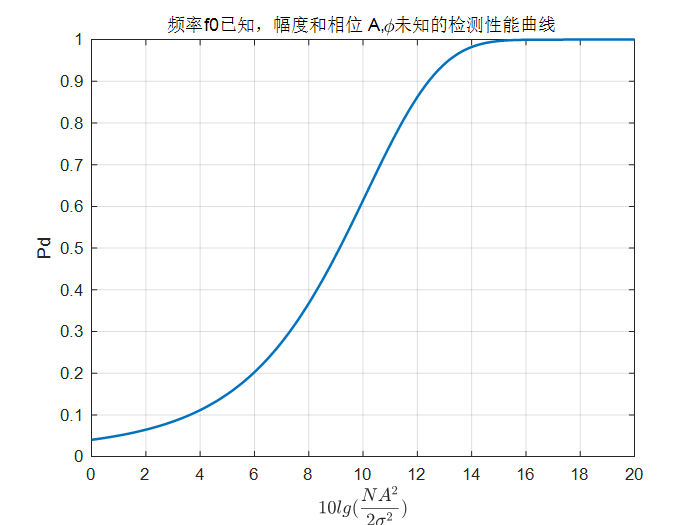
\includegraphics[scale=0.7]{4.1.png}
	\caption{频率\(f_0\)已知,幅度A和相位\(\phi\)未知的检测性能曲线}
	\label{5.4.1}
\end{figure}

\subsubsection*{(2)若频率\(f_0\)及幅度相位\(A,\phi \)均未知(假定\(0<f_0<1/2,A>0\)),若\(\sigma^2=1,N=20\),虚警概率设定为\(0.01\),分析检测门限及检测概率并仿真.}

第二问在第一问的基础上更改了初始条件,即频率\(f_0\)未知,推导过程与第一问类似,而\(\alpha_1=\frac{2}{N}\sum_{k=0}^{N-1}z(k)\cos 2\pi f_0k,\alpha_2=\frac{2}{N}\sum_{k=0}^{N-1}z(k)\sin 2\pi f_0k\),这两个量由于\(f_0\)未知,需要遍历\(0<f_0<1/2\)。因此最终用周期图简化判决准则的时候有所不同:
\begin{align*}
	\begin{matrix}
		\max \\f_0
	\end{matrix}
	I(f_0)
	\begin{matrix}
		\mathcal{H}_1 \\
		>             \\
		<             \\
		\mathcal{H}_0
	\end{matrix}
	\sigma^2 \ln \gamma=\gamma^{\prime}
\end{align*}

如果超过判决门限,则判定\(\mathcal{H}_1\),如果周期图峰值超过门限,检测器判存在正选信号,如果是这样,则峰值所处的频率是频率值的最大似然估计。这就解释了为什么周期图或者它的快速傅里叶变换实现几乎是所有窄带检测系统的组成部分。与第一问的差别是虚警率\(P_F\)随搜索频率单元数增加而增加,其中\(L=I(N/2-1)\),I是多普勒单元数,\((N/2-1)\)是距离单元数
\begin{align*}
	P_F=1-(1-\exp(-\frac{\gamma^{\prime}}{\sigma^2}))^L\approx 1-(1-L\exp(-\frac{\gamma^{\prime}}{\sigma^2}))=LP_F(bin)
\end{align*}

假定N点FFT用来计算周期图\(I(f)\),且仅考虑单元扫描,则最大值在频率\(f_k=\frac{k}{N}\)上求得,其中\(k=1,2,\ldots, N/2-1\)。我们有

\begin{align*}
	P_D=Q_{\chi^{\prime2}_2(\frac{NA^2}{2\sigma^2})}(2\ln \frac{N/2-1}{P_F})
\end{align*}
检测性能曲线仿真如下:

\begin{figure}[H]
	\centering
	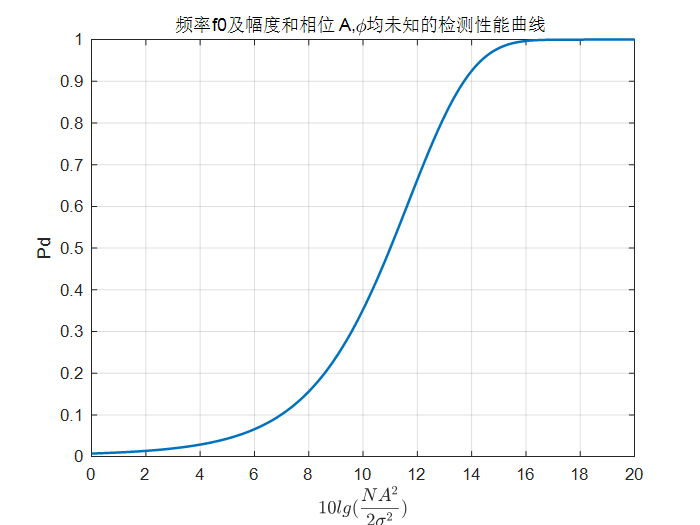
\includegraphics[scale=0.7]{4.2.png}
	\caption{频率\(f_0\),幅度A和相位\(\phi\)均未知的检测性能曲线}
	\label{5.4.2}
\end{figure}

将第一问与第二问的结果放在一起进行比较:

\begin{figure}[H]
	\centering
	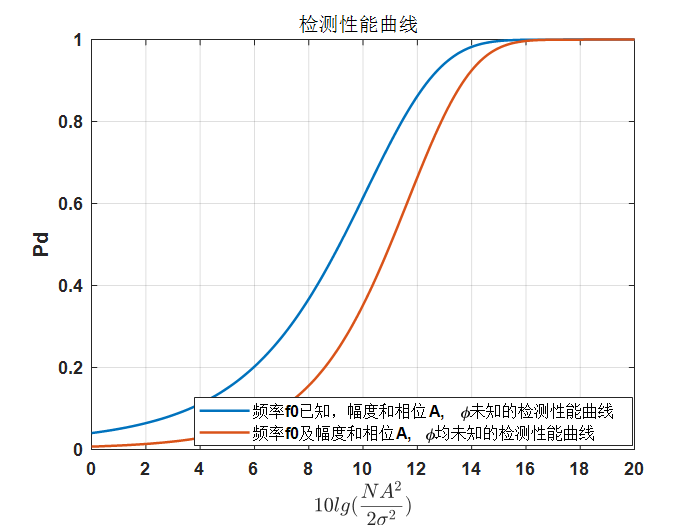
\includegraphics[scale=0.7]{4.3.png}
	\caption{检测性能曲线}
	\label{6.4.3}
\end{figure}

可见未知参数越多检测性能越差,且对于频率未知的检测而言,N值越大检测性能越大。

\section{未知信号检测}
\subsection{第一题:信号分布已知的NP检验}
考虑二元假设问题

\begin{align*}
	\begin{matrix}
		\mathcal{H}_0: & z[k]=n[k]      \\
		\mathcal{H}_1: & z[k]=s[k]+n[k]
	\end{matrix}\quad k=0,1,\ldots,N-1
\end{align*}
噪声是服从\(n(k)\sim \mathcal{N}(0,\sigma^2)\)的WGN。

\subsubsection*{(1)若\(s[k]=A,A\sim \mathcal{N}(0,\sigma^2_A)\)且与噪声独立,\(\sigma^2_A\)已知,求解NP判决式。}

参照例5.1,由于信号服从\(A\sim \mathcal{N}(0,\sigma^2_A)\)的WGN,所以在\(\mathcal{H}_0\)条件下,\(\mathbf{z}\sim \mathcal{N}(\mathbf{0},\sigma^2\mathbf{I})\),在\(\mathcal{H}_1\)条件下,\(\mathbf{z}\sim \mathcal{N}(\mathbf{0},(\sigma^2+\sigma^2_A)\mathbf{I})\),

根据NP准则,如果似然比超过门限
\begin{align*}
	L(\mathbf{z})=\frac{p(\mathbf{z};\mathcal{H}_1)}{p(\mathbf{z};\mathcal{H}_0)}>\gamma
\end{align*}
则NP检测器判\(\mathcal{H}_1\)。
其中
\begin{align*}
	p(\mathbf{z};\mathcal{H}_1)
	 & =\frac{1}{[2\pi (\sigma_A^2+\sigma^2)]^{N/2}}\exp
	\left[-\frac{1}{2(\sigma^2_s+\sigma^2)}\sum_{n=0}^{N-1}z^2[n] \right] \\
	p(\mathbf{z};\mathcal{H}_0)
	 & =\frac{1}{(2\pi\sigma^2)^{N/2}}\exp
	\left[-\frac{1}{2\sigma^2}\sum_{n=0}^{N-1}z^2[n] \right]
\end{align*}
对数似然比可以求得
\begin{align*}
	\ln L(\mathbf{z})
	 & =\frac{N}{2}\ln(\frac{\sigma^2}{\sigma^2+\sigma^2_A})-
	\frac{1}{2}(\frac{1}{\sigma^2_s+\sigma^2}-\frac{1}{\sigma^2})\sum_{n=0}^{N-1}z^2[n] \\
	 & =\frac{N}{2}\ln(\frac{\sigma^2}{\sigma^2+\sigma^2_A})
	+\frac{1}{2}\frac{\sigma^2_A}{(\sigma^2_A+\sigma^2)\sigma^2}\sum_{n=0}^{N-1}z^2[n]
\end{align*}
如果
\begin{align*}
	T(\mathbf{z})=\sum_{n=0}^{N-1}z^2[n]>2\sigma^2(1+\frac{\sigma^2}{\sigma^2_A})\left[\ln \gamma+\frac{N}{2}\ln(1+\frac{\sigma^2_A}{\sigma^2})\right]=\gamma^{\prime}
\end{align*}
则\(\mathcal{H}_1\)成立。

\subsubsection*{(2)若\(s[k]\sim Ar^k(0<r<1),A\sim \mathcal{N}(0,\sigma^2_A)\)且与噪声独立,\(\sigma^2_A\)已知,求解NP判决式。}

若\(s[k]\sim Ar^k(0<r<1)\),假设可以重写为线性模型
\begin{align*}
	\mathcal{H}_0 & :\mathbf{z}=\mathbf{n}             \\
	\mathcal{H}_1 & :\mathbf{z}=\mathbf{H}A+\mathbf{n}
\end{align*}
其中
\begin{align*}
	\mathbf{z}=
	 & \begin{bmatrix}
		   z[0] & z[1] & \cdots & z[N-1]
	   \end{bmatrix}^T \\
	\mathbf{n}=
	 & \begin{bmatrix}
		   n[0] & n[1] & \cdots & n[N-1]
	   \end{bmatrix}^T \\
	\mathbf{H}=
	 & \begin{bmatrix}
		   0 & r & \cdots & r^k
	   \end{bmatrix}^T
\end{align*}
由于\(A\sim \mathcal{N}(0,\sigma^2_A)\)且与噪声独立,所以
\begin{align*}
	\mathbf{z}\sim\left\{
	\begin{matrix}
		\mathcal{N}(\mathbf{0},\sigma^2\mathbf{I})                         & ,\mathcal{H}_0 \\
		\mathcal{N}(\mathbf{0},\sigma^2_A\mathbf{HH}^T+\sigma^2\mathbf{I}) & ,\mathcal{H}_1
	\end{matrix}
	\right.
\end{align*}

类似第\(\mathbf{(1)}\)问,根据NP准则,如果似然比
\begin{align*}
	L(\mathbf{z})=\frac{p(\mathbf{z};\mathcal{H}_1)}{p(\mathbf{z};\mathcal{H}_0)}>\gamma
\end{align*}
则NP检测器判\(\mathcal{H}_1\)。其中
\begin{align*}
	p(\mathbf{z};\mathcal{H}_1)
	 & =\frac{1}{(2\pi)^{N/2} \det^{1/2}(\sigma^2_A\mathbf{HH}^T+\sigma^2\mathbf{I})}
	\exp\left[-\frac{1}{2}\mathbf{z}^T(\sigma^2_A\mathbf{HH}^T+\sigma^2\mathbf{I})^{-1}\mathbf{z} \right] \\
	p(\mathbf{z};\mathcal{H}_0)
	 & =\frac{1}{(2\pi\sigma^2)^{N/2}}\exp
	\left(-\frac{1}{2\sigma^2}\mathbf{z}^T\mathbf{z} \right)
\end{align*}
对数似然比可以求得
\begin{align*}
	\ln L(\mathbf{z})
	 & =-N\ln(\sigma)+\frac{1}{2}\ln \det(\sigma^2_A\mathbf{HH}^T+\sigma^2\mathbf{I})
	-\frac{1}{2}\mathbf{z}^T(\sigma^2_A\mathbf{HH}^T+\sigma^2\mathbf{I})^{-1}\mathbf{z}
	+\frac{\mathbf{z}^T\mathbf{z}}{{2\sigma^2}}                                       \\
	 & =-N\ln(\sigma)+\frac{1}{2}\ln(\sigma^2+\sigma^2_A\mathbf{HH}^T)
	+\frac{1}{2}\mathbf{z}^T\left[-(\sigma^2_A\mathbf{HH}^T+\sigma^2\mathbf{I})^{-1}+\frac{1}{\sigma^2}\mathbf{I}\right]\mathbf{z}
\end{align*}
利用矩阵求逆引理
\begin{align*}
	(\mathbf{A}+\mathbf{BCD})^{-1}=A^{-1}-\mathbf{A}^{-1}\mathbf{B}(\mathbf{DA}^{-1}\mathbf{B}+\mathbf{C}^{-1})^{-1}\mathbf{DA}^{-1}
\end{align*}
令\(\mathbf{A}=\sigma^2\mathbf{I},\mathbf{B}=\mathbf{H},\mathbf{D}=\mathbf{H}^T,\mathbf{C}=\sigma^2_A\mathbf{I}\),得到
\begin{align*}
	(\sigma^2_A\mathbf{HH}^T+\sigma^2\mathbf{I})^{-1}
	 & =\frac{1}{\sigma^2}\mathbf{I}-
	\frac{1}{\sigma^2}\mathbf{IH}(\mathbf{H}^T\frac{1}{\sigma^2}\mathbf{IH}+\frac{1}{\sigma^2_A}\mathbf{I})^{-1}
	\mathbf{H}^T\frac{1}{\sigma^2}\mathbf{I}                                                                                                \\
	 & =\frac{1}{\sigma^2}\mathbf{I}-\frac{\sigma^2_A\mathbf{H}^T\mathbf{H}}{\sigma^2(\sigma^2+\sigma^2_A\mathbf{H}^T\mathbf{H})}\mathbf{I} \\
	 & =\frac{\mathbf{I}}{\sigma^2+\sigma^2_A\mathbf{H}^T\mathbf{H}}
\end{align*}
所以对数似然函数
\begin{align*}
	\ln L(\mathbf{z})
	 & =-N\ln(\sigma)+\frac{1}{2}\ln(\sigma^2+\sigma^2_A\mathbf{HH}^T)
	+\frac{1}{2}(-\frac{1}{\sigma^2+\sigma^2_A\mathbf{H}^T\mathbf{H}}+\frac{1}{\sigma^2})\mathbf{z}^T\mathbf{z}        \\
	 & =-N\ln(\sigma)+\frac{1}{2}\ln(\sigma^2+\sigma^2_A\mathbf{HH}^T)+
	\frac{\sigma^2_A\mathbf{H}^T\mathbf{H}}{\sigma^2(\sigma^2+\sigma^2_A\mathbf{H}^T\mathbf{H})}\mathbf{z}^T\mathbf{z} \\
	 & >\ln \gamma
\end{align*}
时,判\(\mathcal{H}_1\)。

由于\(\sigma^2,\sigma^2_A\)均已知,可以整理为
\begin{align*}
	T(\mathbf{z}) & =\mathbf{z}^T\mathbf{z}                                                                       \\
	              & >\frac{\sigma^2(\sigma^2+\sigma^2_A\mathbf{H}^T\mathbf{H})}{\sigma^2_A\mathbf{H}^T\mathbf{H}}
	(\ln \gamma+N\ln (\sigma)-\frac{1}{2}\ln(\sigma^2+\sigma^2_A\mathbf{HH}^T))                                   \\
	              & =\gamma^{\prime\prime}
\end{align*}
则\(\mathcal{H}_1\)成立。其中\(\mathbf{H}^T\mathbf{H}=\sum_{k=0}^{N-1}r^{2k}=\frac{1-r^{2N}}{1-r^2}\)。

\subsubsection*{(3)若\(s[k]=A\cos(2\pi f_0 k+\phi )\),A已知但\(\phi\)未知,若检验统计量采用\(\sum_{k=0}^{N-1}z[k]A\cos(2\pi f_0 k)\),讨论大N情况下偏移系数及其与\(\phi\)的关系。}
假设\(\phi\)服从均匀分布,\(\phi\sim \mathcal{U}(0,2\pi)\),则\(E\left[\cos(\phi)\right]=E\left[\sin(\phi)\right]=0\)

\begin{align*}
	E(T;\mathcal{H}_1)
	 & =E\left[\sum_{k=0}^{N-1}z[k]A\cos (2\pi f_0 k)\right]                                        \\
	 & =E\left[\sum_{k=0}^{N-1}(s[k]+n[k])A\cos (2\pi f_0 k)\right]                                 \\
	 & =E\left[\sum_{k=0}^{N-1}A^2\cos(2\pi f_0 k+\phi)\cos (2\pi f_0 k)\right]                     \\
	 & =E\left\{\sum_{k=0}^{N-1}\frac{A^2}{2}\left[\cos(4\pi f_0 k+\phi)+\cos (\phi)\right]\right\} \\
	 & =\frac{NA^2}{2}\cos(\phi)+E\left[\sum_{k=0}^{N-1}\frac{A^2}{2}\cos(4\pi f_0 k+\phi)\right]   \\
	 & =\frac{NA^2}{2}\cos(\phi)
\end{align*}

\begin{align*}
	E(T;\mathcal{H}_0)
	 & =E\left[\sum_{k=0}^{N-1}z[k]A\cos (2\pi f_0 k)\right] \\
	 & =E\left[\sum_{k=0}^{N-1}n[k]A\cos (2\pi f_0 k)\right] \\
	 & =0
\end{align*}
由于噪声\(n[k]\sim\mathcal{N}(0,\sigma^2)\)的WGN,所以\(E\left[n[k]n[l]\right]=\delta(k,l)\sigma^2\)
\begin{align*}
	Var(T;\mathcal{H}_0)
	 & =E\left\{\left[\sum_{k=0}^{N-1}z[k]A\cos (2\pi f_0 k)\right]^2 \right\}-E^2\left[\sum_{k=0}^{N-1}z[k]A\cos (2\pi f_0 k)\right] \\
	 & =A^2E\left[\sum_{k=0}^{N-1}\sum_{l=0}^{N-1}n[k]n[l]\cos (2\pi f_0 k)\cos (2\pi f_0 l)\right]                                   \\
	 & =A^2\sigma^2\sum_{k=0}^{N-1}\cos^2 (2\pi f_0 k)                                                                                \\
	 & =\frac{A^2\sigma^2}{2}\sum_{k=0}^{N-1}1+\cos (4\pi f_0 k)
\end{align*}
对于大的N值
\begin{align*}
	\frac{1}{N}\sum_{k=0}^{N-1}\cos k\alpha
	 & =\frac{1}{N}Re\left(\sum_{k=0}^{N-1}\exp(jk\alpha)\right)                             \\
	 & =\frac{1}{N}Re\left[\exp(j(N-1)\alpha/2)\frac{\sin(N\alpha/2)}{\sin(\alpha/2)}\right] \\
	 & \approx \frac{\sin(N\alpha)}{2N\sin(\alpha/2)}
\end{align*}
所以
\begin{align*}
	Var(T;\mathcal{H}_0)
	 & \approx \frac{A^2\sigma^2}{2}(N+\frac{\sin(N\alpha)}{2\sin(\alpha/2)}) \\
	 & \approx\frac{NA^2\sigma^2}{2}
\end{align*}

偏移系数
\begin{align*}
	d^2
	 & =\frac{\left[E(T;\mathcal{H}_1)-E(T;\mathcal{H}_0)\right]^2}{Var(T;\mathcal{H}_0)} \\
	 & =\frac{NA^2}{2\sigma^2}\cos^2 \phi
\end{align*}
偏移系数与\(\phi\)有关,当\(\phi=0,\pi\)时,检测性能最佳,当\(\phi=\pi/2,3\pi/2\)时,检测性能最差。

这是由于检验统计量\(\sum_{k=0}^{N-1}z[k]A\cos(2\pi f_0 k)\)不能构成单一的充分统计量。

由于\(s[n]=A\cos (2\pi f_0 k+\phi)\),
\begin{align*}
	p(\mathbf{z};\mathcal{H}_1)
	=  \frac{1}{(2\pi \sigma^2)^{N/2}}
	 & \exp\left\{-\frac{1}{2\sigma^2}\sum_{k=0}^{N-1}[z[n]-A\cos (2\pi f_0 k+\phi)]^2 \right\}                                                        \\
	=  \frac{1}{(2\pi \sigma^2)^{N/2}}
	 & \exp\bigg\{-\frac{1}{2\sigma}\bigg[\sum_{k=0}^{N-1}z^2[n]-2A\left(\sum_{k=0}^{N-1}z[n]\cos2\pi f_0 k\right)\cos \phi                            \\
	 & +2A\left(\sum_{k=0}^{N-1}z[n]\sin 2\pi f_0 k\right)\sin \phi\bigg] +\sum_{k=0}^{N-1}A^2\cos^2 (2\pi f_0 k +\phi)\bigg\}                         \\
	= \frac{1}{(2\pi \sigma^2)^{N/2}}
	 & \exp\left\{-\frac{1}{2\sigma^2}\left[\sum_{k=0}^{N-1}A^2\cos(2\pi f_0 k+\phi)-2T_1(\mathbf{z})\cos\phi+2T_2(\mathbf{z})\sin \phi\right]\right\} \\
	 & \cdot \exp\left[-\frac{1}{2\sigma^2}\sum_{k=0}^{N-1}z^2[n]\right]                                                                               \\
	 & =g(T(\mathbf{z}),T_2(\mathbf{z}),\phi)\cdot h(\mathbf{z})
\end{align*}
其中
\begin{align*}\
	T_1(\mathbf{z}) & =\sum_{k=0}^{N-1}Az[n]\cos2\pi f_0 k \\
	T_2(\mathbf{z}) & =\sum_{k=0}^{N-1}Az[n]\sin2\pi f_0 k
\end{align*}

根据Neyman-Fisher因子分解定理,\(T_1(\mathbf{z})\)和\(T_2(\mathbf{z})\)共同构成充分统计量,单一的\(T_1(\mathbf{z})\)并没有包含进行NP假设检验的所有信息。

\subsection{第二题:信号形式或功率谱密度已知的GLRT检验}
考虑二元假设检验问题

\begin{align*}
	\begin{matrix}
		H_0: & z(k)=n(k)      \\
		H_1: & z(k)=s[k]+n(k)
	\end{matrix}\quad k=0,1,\cdots N-1
\end{align*}
其中噪声\(n(k)\)是服从\(n(k)\sim \mathcal{N}(0,\sigma^2)\)的WGN。

\subsubsection*{(1)若\(s[k]=Ar^k,r\)已知且\(0<r<1,A\sim \mathcal{N}(0,\sigma^2_A),\sigma^2_A\)未知且与噪声A独立,求GLRT判决式}

可重写为线性模型
\begin{align*}
	\mathcal{H}_0: & \mathbf{z}=\mathbf{n}             \\
	\mathcal{H}_1: & \mathbf{z}=\mathbf{H}A+\mathbf{n}
\end{align*}
其中\(\mathbf{H}=\begin{bmatrix}1&r&\cdots&r^{N-1}\end{bmatrix}^T,\mathbf{H}A\sim\mathcal{N}(\mathbf{0},\mathbf{C}_s),\mathbf{C}_s=\sigma^2_A\mathbf{HH}^T\)。记\(\mathbf{C}=\mathbf{HH}^T,P_0=\sigma^2_A\)。则在\(\mathcal{H}_1\)假设下的PDF
\begin{align*}
	p(\mathbf{z};P_0,\mathcal{H}_1)
	=\frac{1}{(2\pi )^{N/2}\det^{1/2}(P_0\mathbf{C}+\sigma^2\mathbf{I})}
	\exp\left[-\frac{1}{2}\mathbf{z}^T(P_0\mathbf{C}+\sigma^2\mathbf{I})^{-1}\mathbf{z}\right]
\end{align*}

考虑\(\mathbf{C}\)的正交相似对角化\(\mathbf{V}^T\mathbf{C}\mathbf{V}=\Lambda\)。
\begin{align*}
	\det(P_0\mathbf{C}+\sigma^2\mathbf{I})
	 & =\det\left(P_0\mathbf{V}\Lambda\mathbf{V}^{-1}+\sigma^2\mathbf{I}\right) \\
	 & =\det[\mathbf{V}(P_0\Lambda+\sigma^2\mathbf{I})\mathbf{V}^{-1}]          \\
	 & =\det(P_0\Lambda+\sigma^2\mathbf{I})                                     \\
	 & =\prod_{i=1}^{N}(P_0\lambda_i+\sigma^2)
\end{align*}
另外,我们有
\begin{align*}
	(P_0\mathbf{C}+\sigma^2\mathbf{I})^{-1}
	 & =(P_0\mathbf{V}\Lambda\mathbf{V}^{-1}+\sigma^2\mathbf{I})^{-1} \\
	 & =[\mathbf{V}(P_0\Lambda+\sigma^2\mathbf{I})\mathbf{V}^{-1}]    \\
	 & =\mathbf{V}(P_0\Lambda+\sigma^2\mathbf{I})^{-1}\mathbf{V}^T
\end{align*}
对数似然函数
\begin{align*}
	\ln p(\mathbf{z};P_0.\mathcal{H}_1)
	 & =-\frac{N}{2}\ln 2\pi -\frac{1}{2}\sum_{i=1}^{N-1}\ln
	(P_0\lambda_i)-\frac{1}{2}\mathbf{z}^T\mathbf{V}(P_0\Lambda+\sigma^2\mathbf{I})^{-1}\mathbf{V}^T\mathbf{z} \\
	 & =-\frac{N}{2}\ln 2\pi -\frac{1}{2}\sum_{i=1}^{N-1}\ln(P_0\lambda_i+\sigma^2)
	-\frac{1}{2}\sum_{i=1}^{N}\frac{(\mathbf{v}^T_i\mathbf{z})^2}{P_0\lambda_i+\sigma^2}
\end{align*}
为了求得\(P_0=\sigma^2_A\)的MLE,需要使得
\begin{align*}
	J(P_0)=\sum_{i=1}^{N-1}\ln(P_0\lambda_i+\sigma^2)
	+\frac{(\mathbf{v}^T_i\mathbf{z})^2}{P_0\lambda_i+\sigma^2}\to min
\end{align*}
由于\(\text{rank}(\mathbf{C})=\text{rank}(\mathbf{HH}^T)=1\),因此有\(\lambda_1\neq 0,\lambda_i=0,i=2,3,\cdots, N\)。对于秩为1的协方差矩阵,\(P_0\)的MLE通过使下式最小得到
\begin{align*}
	J(P_0)=\ln(P_0\lambda_1+\sigma^2)+\sigma^2+\frac{(\mathbf{v}_1^T\mathbf{z})^2}{P_0\lambda_1+\sigma^2}
	+(N-1)\ln \sigma^2+\sigma^{-2}\sum_{i=2}^{N-1}(\mathbf{v}_i^T\mathbf{z})^2
\end{align*}
求导令上式为零,只要\(\hat{P}_0>0\),就有
\begin{align*}
	\hat{P}_0=\frac{(\mathbf{v}_1^T\mathbf{z})^2-\sigma^2}{\lambda_1}
\end{align*}
由于\(P_0=\sigma^2_A\geq0\),因此
\begin{align*}
	\hat{P}_0=\max(0,\frac{(\mathbf{v}_1^T\mathbf{z})^2-\sigma^2}{\lambda_1})
\end{align*}
记\(\hat{P}_0^+=\frac{(\mathbf{v}_1^T\mathbf{z})^2-\sigma^2}{\lambda_1}\),似然比为
\begin{align*}
	L_G(\mathbf{z})=\frac{\frac{1}{(2\pi)^{N/2}\det^{1/2}(\hat{P_0}\mathbf{C}+\sigma^2\mathbf{I})}
		\exp\left[-\frac{1}{2}\mathbf{z}^T(\hat{P}_0\mathbf{C}+\sigma^2\mathbf{I})^{-1}\mathbf{z}\right]}
	{(2\pi \sigma^2)({-N/2})\exp\left(-\frac{1}{2}\mathbf{z}^T\mathbf{z}\right)}
\end{align*}
对数似然比
\begin{align*}
	\ln L_G(\mathbf{z})
	 & =-\frac{1}{2}J(\hat{P}_0)+\frac{N}{2}\ln \sigma^2+(2\sigma^2)^{-1}\mathbf{z}^T\mathbf{z}                                                               \\
	 & =-\frac{1}{2}\ln(\hat{P}_0\lambda_1+\sigma^2)-\frac{1}{2}\frac{(\mathbf{v}_1^T\mathbf{z})}{\hat{P_0\lambda_1+\sigma^2}}
	-\frac{N-1}{2}\ln \sigma^2-\frac{1}{2\sigma^2}\sum_{i=2}^{N}(\mathbf{v}_i^T\mathbf{z})^2+\frac{N}{2}\ln\sigma^2+\frac{1}{2\sigma^2}\mathbf{z}^T\mathbf{z} \\
	 & =-\frac{1}{2}\ln\left(\frac{\hat{P}_0\lambda_1}{\sigma^2}+1\right)-\frac{1}{2}\frac{\hat{P}_0^+\lambda_1+\sigma^2}{\hat{P}_0\lambda_1+\sigma^2}
	+\frac{1}{2\sigma^2}\left(\mathbf{z}^T\mathbf{z}-\sum_{i=2}^{N}\mathbf{z}^T\mathbf{v}_i\mathbf{v}_i^T\mathbf{z}\right)
\end{align*}
\(\mathbf{VV}^T=\sum_{i-1}^{N}=\mathbf{I}\),所以\(\mathbf{I}-\sum_{i=2}^{N}\mathbf{v}_i\mathbf{v}_i^T=\mathbf{v}_1\mathbf{v}_1^T\)。利用这一结果可得判决表达
\begin{align*}
	\ln L_G(\mathbf{z})
	 & =-\frac{1}{2}\ln\left(\frac{\hat{P}_0\lambda_1}{\sigma^2}+1\right)
	-\frac{1}{2}\frac{\hat{P}_0^+\lambda_1+\sigma^2}{\hat{P}_0\lambda_1+\sigma^2}
	+\frac{1}{2\sigma^2}\left(\mathbf{v}_1^T\mathbf{z}\right)^2                                                                              \\
	 & =-\frac{1}{2}\ln\left(\frac{\hat{P}_0\lambda_1}{\sigma^2}+1\right)
	-\frac{1}{2}\frac{\hat{P}_0^+\lambda_1+\sigma^2}{\hat{P}_0\lambda_1+\sigma^2}
	+\frac{1}{2}\frac{\hat{P}_0^+\lambda_1+\sigma^2}{\sigma^2}                                                                               \\
	 & =\frac{1}{2}\left[(\hat{P}_0^+\lambda_1+\sigma^2)(\frac{1}{\sigma^2}-\frac{1}{\hat{P}_0^++\sigma^2})
	-\ln\left(\frac{\hat{P}_0^+\lambda_1+\sigma^2}{\sigma^2}+1\right)\right]                                                                 \\
	 & =\frac{1}{2}\left[\left(\frac{\hat{P}_0^+\lambda_1+\sigma^2}{\hat{P}_0\lambda_1+\sigma^2}\frac{\hat{P}_0\lambda_1}{\sigma^2}+1\right)
		-\ln\left(\frac{\hat{P}_0^+\lambda_1+\sigma^2}{\sigma^2}+1\right)-1\right]
	\begin{matrix}
		\mathcal{H}_1 \\>\\<\\\mathcal{H}_0
	\end{matrix}\ln \gamma
\end{align*}
如果\(\hat{P}_0=0\),那么\(\ln L_G(\mathbf{z})=0\),由于\(\ln\gamma>0\),此时判为\(\mathcal{H}_0\)。如果\(\hat{P}_0>0\),此时\(\hat{P}_0=\hat{P}_0^+\),
\begin{align*}
	\ln L_G(\mathbf{z})
	 & =\frac{1}{2}\left[(\frac{\hat{P}_0\lambda_1}{\sigma^2}+1)-\ln(\frac{\hat{P}_0\lambda_1}{\sigma^2}+1)-1\right]
	\begin{matrix}
		\mathcal{H}_1 \\>\\<\\\mathcal{H}_0
	\end{matrix}\ln \gamma
\end{align*}
当\(x>1\)时,\(g(x)=x-\ln x-1\)是单调递增的函数,因此等价判决为
\begin{align*}
	\hat{P}_0>\frac{\sigma^2}{\lambda_1}[g^{-1}(2\ln \gamma)-1]=\gamma
\end{align*}
这等价于
\begin{align*}
	T(\mathbf{z})=(\mathbf{v}_1^T\mathbf{z})^2
	\begin{matrix}
		\mathcal{H}_1 \\>\\<\\\mathcal{H}_0
	\end{matrix}\gamma^{\prime\prime}
\end{align*}
可以求得
\begin{align*}
	\lambda_1
	 & =\mathbf{H}^T\mathbf{H}=\sum_{i=0}^{N-1}r^i \\
	\mathbf{v}_1
	 & =\begin{bmatrix}
		    1 & r & \cdots r^{N-1}
	    \end{bmatrix}^T/\mathbf{H}^T\mathbf{H}
	=\frac{1}{\sum_{i=0}^{N-1}r^i}
	\begin{bmatrix}
		1 & r & \cdots r^{N-1}
	\end{bmatrix}^T
\end{align*}
从而
\begin{align*}
	T(\mathbf{z})=(\mathbf{v}_1^T\mathbf{z})^2=\frac{\sum_{i=1}^{N-1}z[k]r^k}{\frac{1-r^{2N}}{1-r^2}}
	\begin{matrix}
		\mathcal{H}_1 \\>\\<\\\mathcal{H}_0
	\end{matrix} \gamma^{\prime\prime}
\end{align*}

\subsubsection*{(2)若\(s[k]\)是广义平稳随机过程,其功率谱密度
	\begin{align*}
		P_s(f;P_0)=\left\{
		\begin{matrix}
			2P_0 & 0\leqslant f\leqslant 1/4 \\
			0    & 1/4<f\leqslant1/2
		\end{matrix}\right.
	\end{align*}
	其中\(P_0\)未知,求GLRT判决式。}

对于信号是WSS时的大数据记录下的情况,对数似然比
\begin{align*}
	\ln \Lambda_G(\mathbf{z})=\ln \frac{p(\mathbf{z};\mathcal{H}_1)}{p(\mathbf{z};\mathcal{H}_0)}
	=\frac{N}{2}\int_{-1/2}^{1/2}\ln (\frac{P_{ss}(f)}{\sigma^2}+1)-\frac{P_{ss}(f)}{P_{ss}+\sigma^2}\frac{I(f)}{\sigma^2}df
\end{align*}
\(\hat{P}_0\)的MLE可通过使下式最小得到
\begin{align*}
	J(P_0)=\int_{-1/2}^{1/2}\ln (\frac{P_{ss}(f)}{\sigma^2}+1)-\frac{P_{ss}(f)}{P_{ss}+\sigma^2}\frac{I(f)}{\sigma^2}df
\end{align*}
其中\(I(f)\)为周期图
\begin{align*}
	I(f) & =\frac{1}{N}|\sum_{k=0}^{N-1}z[k]\exp(-j2\pi fk)|^2
\end{align*}
\begin{align*}
	J(P_0)
	 & =\int_{0}^{1/4}\ln (\frac{2P_0}{\sigma^2}+1)-\frac{2P_0}{2P_0+\sigma^2}\frac{I(f)}{\sigma^2}df                           \\
	 & =\int_{0}^{1/4}\ln (\frac{2P_0}{\sigma^2}+1)-\frac{I(f)}{\sigma^2}+\frac{\sigma^2}{2P_0+\sigma^2}\frac{I(f)}{\sigma^2}df \\
	 & =\int_{0}^{1/4}\ln (\frac{2P_0}{\sigma^2}+1)-\frac{I(f)}{\sigma^2}+\frac{I(f)}{2P_0+\sigma^2}df
\end{align*}
对\(P_0\)求导,令一阶导数为零得到
\begin{align*}
	\frac{\partial J(P_0)}{\partial P_0}
	 & =\int_{0}^{1/4}\frac{2}{2P_0+\sigma^2}-\frac{2I(f)}{(2P_0+\sigma^2)^2}df
\end{align*}
得到\(\hat{P}_0\)的MLE 为
\begin{align*}
	\hat{P}_0=2\int_{0}^{1/4}I(f)df-\frac{\sigma^2}{2}
\end{align*}
\begin{align*}
	J(\hat{P}_0)
	 & =\int_{0}^{1/4}\left[\ln(\frac{4\int_{0}^{1/4}I(f)df}{\sigma^2})-\frac{I(f)}{\sigma^2}+\frac{I(f)}{4\int_{0}^{1/4}I(f)df}\right] \\
	 & =\frac{1}{4}\left[\ln(\frac{4\int_{0}^{1/4}I(f)df}{\sigma^2})-\frac{4\int_{0}^{1/4}I(f)df}{\sigma^2}+1\right]
\end{align*}
判决表达可等价于
\begin{align*}
	\frac{4\int_{0}^{1/4}I(f)df}{\sigma^2}-\ln(\frac{4\int_{0}^{1/4}I(f)df}{\sigma^2})-1
	\begin{matrix}
		\mathcal{H}_1 \\>\\<\\\mathcal{H}_0
	\end{matrix} \gamma
\end{align*}

\subsection{第三题:高斯色噪声下的GLRT检验:投影}

高斯噪声中已知信号的分析与仿真,考虑二元假设
\begin{align*}
	\begin{matrix}
		H_0: & z(k)=n(k)      \\
		H_1: & z(k)=s[k]+n(k)
	\end{matrix}\quad k=0,1,\cdots N-1
\end{align*}

噪声是服从\(n(k)\sim \mathcal{N}(0,5)\)的WGN,信号为零均值高斯随机信号,协方差矩阵\([\mathbf{C}]_{ij}=c[i-j],j=0,1,\ldots,N-1\),其中\(c[k]=\frac{1}{1-0.9^2}0.9^{|k|}\),若\(N=100\),虚警概率设定为0.01,试通过计算机模拟分析检测门限及检测概率。

\begin{align*}
	\mathbf{z}\sim\left\{
	\begin{matrix}
		\mathcal{N}(\mathbf{0},\sigma^2\mathbf{I})               & \text{在}\mathcal{H}_0\text{条件下} \\
		\mathcal{N}(\mathbf{0},\mathcal{C}_s+\sigma^2\mathbf{I}) & \text{在}\mathcal{H}_1\text{条件下} \\
	\end{matrix}
	\right.
\end{align*}
似然比
\begin{align*}
	L_G(\mathbf{z})=\frac{\frac{1}{(2\pi)^{N/2}\det^{1/2}(\mathbf{C}_s+\sigma^2\mathbf{I})}
		\exp\left[-\frac{1}{2}\mathbf{z}^T(\mathbf{C}_s+\sigma^2\mathbf{I})^{-1}\mathbf{z}\right]}
	{(2\pi \sigma^2)^{-N/2}\exp\left(-\frac{1}{2}\mathbf{z}^T\mathbf{z}\right)}
	\begin{matrix}
		\mathcal{H}_1 \\>\\<\\\mathcal{H}_0
	\end{matrix} \gamma
\end{align*}
化简得到
\begin{align*}
	T(\mathbf{z})=\mathbf{z}^T\hat{s}>\gamma
\end{align*}
其中
\begin{align*}
	\hat{\mathbf{s}}=\mathbf{C}_s(\mathbf{C}_s+\sigma^2\mathbf{I})^{-1}\mathbf{z}
\end{align*}
从而
\begin{align}
	T(\mathbf{z})=
	\left\{
	\begin{matrix}
		\mathbf{n}^T\hat{\mathbf{s}}              & \text{在}\mathcal{H}_0\text{条件下} \\
		(\mathbf{s}+\mathbf{n})^T\hat{\mathbf{s}} & \text{在}\mathcal{H}_1\text{条件下}
	\end{matrix}
	\right.
\end{align}

\subsection{第四题:能量检测器}

能量检测器的分析与仿真:考虑二元假设
\begin{align*}
	\begin{matrix}
		H_0: & z(k)=n(k)      \\
		H_1: & z(k)=s[k]+n(k)
	\end{matrix}\quad k=0,1,\cdots N-1
\end{align*}
噪声是服从\(n(k)\sim \mathcal{N}(0,\sigma^2)\)的WGN,\(\sigma^2\)已知。

\subsubsection*{(1)若\(s(k)\)是完全未知确定信号,假定\(\sigma^2=1,N=10\),虚警概率设定为0.01,分析检测门限,能得到检测概率吗?}

若\(s(k)\)是完全未知确定信号,则使用最大似然估计\(\hat{s}(k)=z(k)\),似然比为

\begin{align*}
	\Lambda(\mathbf{z})=\frac{p(\mathbf{z}|\hat{s}[0],\hat{s}[2],\ldots,\hat{s}[N-1],\mathcal{H}_1)}{p(\mathbf{z}|\mathcal{H}_0)}
\end{align*}
化简可以得到检测统计量与检测门限为能量检测器的形式:
\begin{align*}
	T(\mathbf{z})=\sum_{n=0}^{N-1}z^2[n]=\sum_{n=0}^{N-1}z[n]z[n]=\sum_{n=0}^{N-1}z[n]\hat{s}[n]>\gamma
\end{align*}
若要得到其检测性能,必须限定一个大前提,即大数据量,小信噪比的时候,近似有
\begin{align*}
	P_D\approx Q[Q^{-1}(P_F)-d^2]
\end{align*}
其中\(d^2=\frac{(\epsilon/\sigma^2)^2}{2N}\),\(\epsilon/\sigma^2\)为信噪比。

虚警概率为0.01的检测概率仿真图如下,其中第一张图是不限定信噪比的检测概率,考虑到检测性能前提,画出了信噪比低于0dB条件下的检测概率曲线,可以看出,检测概率较小。
\begin{figure}[H]
	\centering
	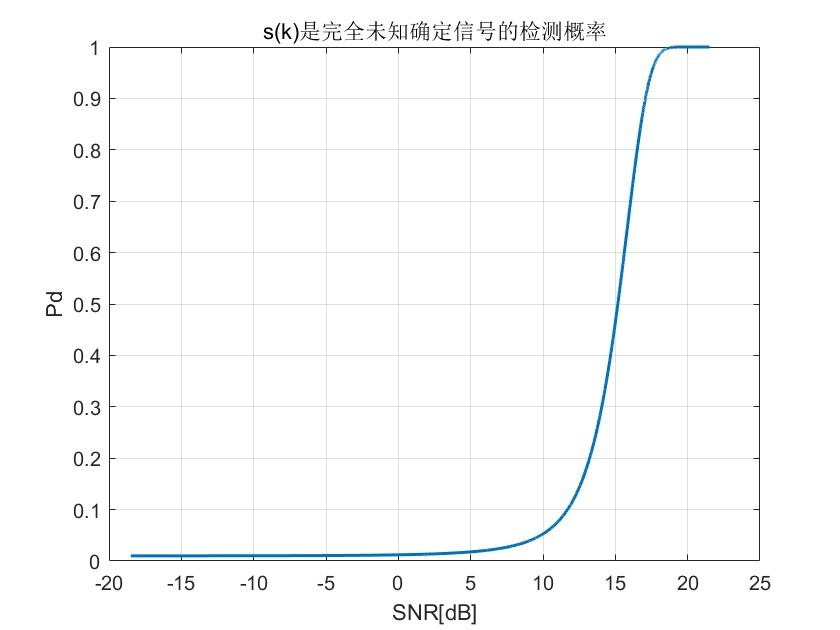
\includegraphics[scale=0.5]{fig4.1.jpg}
	\caption{\(s(k)\)是完全未知确定信号的检测概率}
	\label{6.4.1}
\end{figure}

\begin{figure}[H]
	\centering
	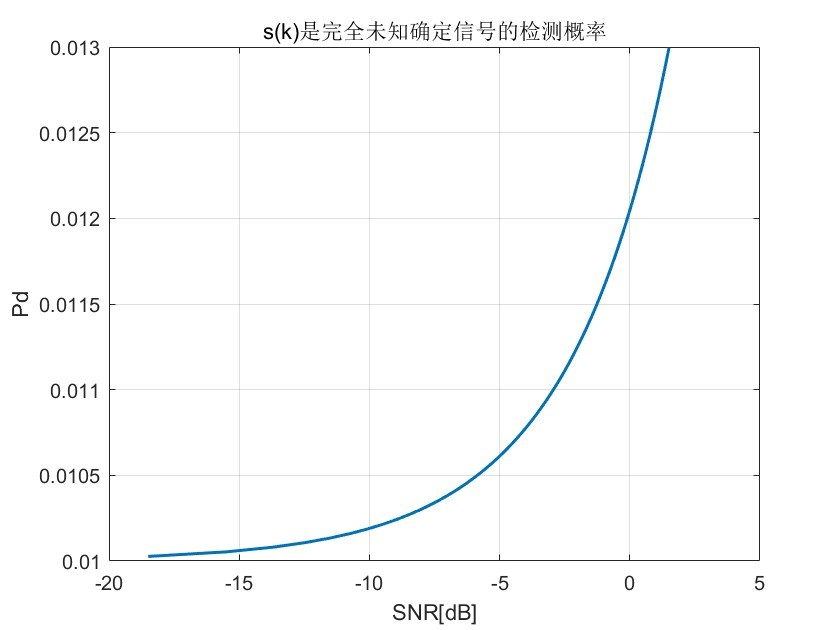
\includegraphics[scale=0.5]{fig4.2.jpg}
	\caption{\(s(k)\)是完全未知确定信号的检测概率}
	\label{6.4.2}
\end{figure}

\subsubsection*{(2)若\(s(k)\)是均值为零方差为\(\sigma^2_s\)的白高斯信号,假定\(\sigma^2=\sigma^2_s=1,N=100\),虚警概率设定为0.01,试分析检测门限及检测概率并仿真。}

若\(s(k)\)是均值为零,方差为\(\sigma^2_s=1\)的高斯白噪声,为典型的高斯白噪声的高斯白噪声随机信号检测,似然比为
\begin{align*}
	\Lambda(\mathbf{z})=\frac{p(\mathbf{z}|\mathcal{H}_1)}{p(\mathbf{z}|\mathcal{H}_0)}>\eta
\end{align*}
由此可以化简得到检验统计量与门限
\begin{align*}
	T(\mathbf{z})=\sum_{n=0}^{N-1}z^2[n]>\gamma
\end{align*}
与确定性信号不同的是,由于信号和噪声均分从高斯分布,则有
\begin{align*}
	\chi^2_N\sim\left\{
	\begin{matrix}
		\frac{T(\mathbf{z})}{\sigma^2}            & , \mathcal{H}_0 \\
		\frac{T(\mathbf{z})}{\sigma^2+\sigma^2_s} & , \mathcal{H}_1
	\end{matrix}
	\right.
\end{align*}
因此虚警概率与检测门限分别为
\begin{align*}
	P_F    & =Pr\{T(\mathbf{z})>\gamma|\mathcal{H}_0\}=Pr\left\{ \frac{T(\mathbf{z})}{\sigma^2}>\frac{\gamma^2}{\sigma^2}|\mathcal{H}_0\right\}=Q_{\chi^2_N}(\frac{\gamma}{\sigma^2}) \\
	\gamma & =\sigma^2Q^{-1}_{\chi^2_N}(P_F)
\end{align*}
检测概率为
\begin{align*}
	P_D
	 & =Pr\left\{T(\mathbf{z})>\gamma|\mathcal{H}_1 \right\}                                                         \\
	 & =Pr\left\{\frac{T(\mathbf{z})}{\sigma^2+\sigma^2_s}<\frac{\gamma}{\sigma^2+\sigma^2_s} |\mathcal{H}_1\right\} \\
	 & =Q_{\chi^2_N}\left(\frac{\gamma}{\sigma^2+\sigma^2_s}\right)                                                  \\
	 & =Q_{\chi^2_N}\left(\frac{\sigma^2Q^{-1}_{\chi^2_N}(P_F)}{\sigma^2+\sigma^2_s}\right)                          \\
	 & =Q_{\chi^2_N}\left(\frac{Q^{-1}_{\chi^2_N}(P_F)}{\sigma^2_s/\sigma^2+1}\right)
\end{align*}
由卡方右尾函数性质可知,当信噪比\(\sigma^2_s/\sigma^2\)增加,检测概率增减,限定虚警概率为0.01条件下,仿真检测性能曲线如下

\begin{figure}[H]
	\centering
	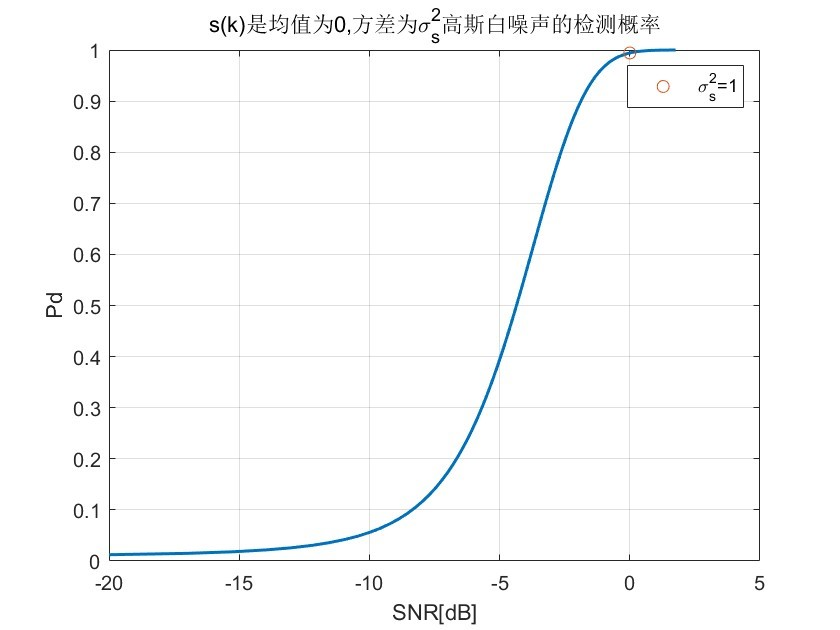
\includegraphics[scale=0.6]{fig4.3.jpg}
	\caption{\(s(k)\)是均值为0,方差为\(\sigma^2_s\)高斯白噪声的检测概率}
	\label{4.3}
\end{figure}

其中当\(\sigma^2=\sigma^2_s=1\)时,门限为135.8067,检测概率\(P_D=99.42\%\)

\section{非高斯信号检测}
\subsection{第一题:GLRT的渐进性能与CFAR}
考虑WGN中二元假设检验问题

\begin{align*}
	\begin{matrix}
		\mathcal{H}_0: & z[k]=n[k]      \\
		\mathcal{H}_1: & z[k]=s[k]+n[k]
	\end{matrix}\quad k=0,1,\ldots,N-1
\end{align*}
噪声是服从\(n(k)\sim \mathcal{N}(0,\sigma^2)\)的WGN。

\subsubsection*{(1)若\(s[k]=A,A\)未知,确定当\(\sigma^2\)已知和未知时的GLRT的渐进性能。}

当\(\sigma^2\)已知时,GLRT计算可以参考课本例6.2与例6.4。

A的最大似然估计为:
\begin{align*}
	\hat{A}=\overline{z}=\frac{1}{N}\sum_{k=0}^{N-1}z(k)
\end{align*}
利用GLRT,我们有
\begin{align*}
	L_G(\mathbf{z})
	=\frac{p(\mathbf{x};A,\mathcal{H}_1)}{p(\mathbf{z};\mathcal{H}_0)}
	=\frac{(2\pi \sigma^2)^{-N/2}\exp\left[-\frac{1}{2\sigma^2}\sum_{n=0}^{N-1}(z[n]-\overline{z})^2\right]}
	{(2\pi \sigma^2)^{-N/2}\exp\left[-\frac{1}{2\sigma^2}\sum_{n=0}^{N-1}z^2[n]\right]}
	\begin{matrix}
		\mathcal{H}_1 \\>\\<\\\mathcal{H_0}
	\end{matrix}\gamma
\end{align*}
取对数化简有:
\begin{align*}
	\ln L_G(\mathbf{z})
	 & =-\frac{1}{2\sigma^2}\left(\sum_{n=0}^{N-1}z^2[n]-
	2\overline{z}\sum_{n=0}^{N-1}z[n]+n\overline{z}^2-\sum_{n=0}^{N-1}z^2[n]\right)             \\
	 & =-\frac{1}{2\sigma^2}(-2N\overline{z}^2+N\overline{z})=\frac{N\overline{z}^2}{2\sigma^2}
	\begin{matrix}
		\mathcal{H}_1 \\>\\<\\\mathcal{H_0}
	\end{matrix}\gamma
\end{align*}
判决条件可以写为
\begin{align*}
	\vert \overline{z}\vert >\gamma
\end{align*}
检验统计量的渐进分布为
\begin{align*}
	2\ln L_G(\mathbf{z})=\frac{N\overline{z}^2}{2\sigma^2}\overset{a}{\sim}
	\left\{\begin{matrix}
		       \chi^2_1                   & \mathcal{H}_0 \\
		       \chi_1^{\prime 2}(\lambda) & \mathcal{H}_1
	       \end{matrix}
	\right.
\end{align*}
其中\(\lambda=\frac{NA^2}{\sigma^2}\),因此对于这种特殊情况,有限数据记录渐进PDF是精确成立的:
\begin{align*}
	\frac{\overline{z}}{\sigma/\sqrt{N}}\sim
	\left\{\begin{matrix}
		       \mathcal{N}(0,1)                        & \mathcal{H}_0 \\
		       \mathcal{N}(\frac{\sqrt{N}A}{\sigma},1) & \mathcal{H}_1
	       \end{matrix}
	\right.
\end{align*}
NP准则确定虚警率与门限的关系为
\begin{align*}
	P_{FA}=2Q\left(\frac{\gamma^{\prime}}{\sqrt{\sigma^2/N}}\right)
\end{align*}
检测概率为
\begin{align*}
	P_D=Q\left[Q^{-1}\left(\frac{P_{FA}}{2}\right)-\sqrt{\frac{NA^2}{\sigma^2}}\right]+
	Q\left[Q^{-1}\left(\frac{P_{FA}}{2}\right)+\sqrt{\frac{NA^2}{\sigma^2}}\right]
\end{align*}

\subsubsection*{(2)若\(s[k]\sim A,A\)未知但已知其取值为-1或1,\(\sigma^2\)未知,求解GLRT判决式并分析是否CFAR。}

当\(\sigma^2\)未知时,GLRT的计算参考教材例6.5,等效检验统计量为\(T(\mathbf{z})=\frac{\overline{z}^2}{\hat{\sigma}^2_1}\)

其PDF并不依赖于\(\sigma^2\),检测性能要比\(\sigma^2\)已知时的检测性能稍差,但在N足够大时,性能衰减是相当小的,基本与\(\sigma^2\)已知时的特性相同,一下是GLRT理论渐进性能与实际渐进性能的比较:

设置信噪比\(\lambda=\frac{NA^2}{\sigma^2}=5,\sigma^2=1\),对于\(N=10,A=\sqrt{\frac{\lambda\sigma^2}{N}}=\sqrt{2}/2\),而对于\(N=30,A=\sqrt{\frac{\lambda\sigma^2}{N}}=\sqrt{6}/6\)。给定虚警概率,分别由理论计算式与蒙特卡洛仿真计算得到的对应检测概率,如图所示

【图】

可见N值越大,GLRT渐进性能越好,N=30时,实际值与理论值十分逼近。

当\(\sigma^2\)未知时,由例9.1可知,\(\sigma^2_0\)和\(\sigma^2_1\)的极大似然估计为
\begin{align*}
	\sigma^2_0 & =\frac{1}{N}\sum_{k=0}^{N-1}z^2[k]           \\
	\sigma^2_1 & =\frac{1}{N}\sum_{k=0}^{N-1}(z[k]-\hat{A})^2
\end{align*}
A的最大似然估计为:
\begin{align*}
	\hat{A}=sgn(\overline{z})
\end{align*}

同1的推导过程
\begin{align*}
	L_G(\mathbf{z})
	 & =\frac{p(\mathbf{z};\hat{A},\hat{\sigma}^2_1,\mathcal{H}_1)}{p(\mathbf{z};\hat{\sigma}^2_0,\mathcal{H}_0)}
	=\frac{(2\pi \hat{\sigma}^2)^{-N/2}\exp\left[-\frac{1}{2\hat{\sigma}^2}\sum_{k=0}^{N-1}(z[k]-sgn(\overline{z}))^2\right]}
	{(2\pi \hat{\sigma}_0^2)^{-N/2}\exp\left[-\frac{1}{2\hat{\sigma}_0^2}\sum_{k=0}^{N-1}z^2[k]\right]}           \\
	 & =\frac{(2\pi \hat{\sigma}^2)^{-N/2}\exp\left(-\frac{N}{2}\right)}
	{(2\pi \hat{\sigma}_0^2)^{-N/2}\exp\left(-\frac{N}{2}\right)}=\left(\frac{\hat{\sigma}_0^2}{\hat{\sigma}_1^2}\right)^{N/2}
	\begin{matrix}
		\mathcal{H}_1 \\>\\<\\\mathcal{H_0}
	\end{matrix}\gamma
\end{align*}

令\(n[k]=\sigma u[k]\),其中\(u[k]\)是方差为1的WGN。在\(\mathcal{H}_0\)条件下,由于\(z[k]=n[k]\),等效检验统计量为
\begin{align*}
	T(\mathbf{z})
	 & =\frac{\overline{z}^2}{\hat{\sigma}^2_1}
	=\frac{\frac{1}{N}\sum_{k=0}^{N-1}z^2[k]}{\frac{1}{N}\sum_{k=0}^{N-1}(z[k]-\hat{A})^2}       \\
	 & =\frac{\frac{1}{N}\sum_{k=0}^{N-1}\sigma^2u^2[k]}
	{\frac{1}{N}\sum_{k=0}^{N-1}(\sigma u[k]-sgn(\sigma \overline{u}))^2}                        \\
	 & =\frac{\sum_{k=0}^{N-1}\sigma^2u^2[k]}{\sum_{k=0}^{N-1}(\sigma u[k]-sgn(\overline{u}))^2}
\end{align*}
其中PDF依赖于\(\sigma^2\),含有未知参数,因此不是CFAR检测器。

\subsubsection*{(3)若\(s[k]=A(-1)^k\),其中A未知,噪声方差\(\sigma^2\)未知,求解GLRT判决式并分析渐进性能。}

与第一问不同之处在于A的最大似然估计形式发生了变化:
\begin{align*}
	\hat{A}=\frac{1}{N}\sum_{k=0}^{N-1}(-1)^kz(k)
\end{align*}
由此,\(\sigma^2_0\)和\(\sigma^2_1\)的最大似然估计也变为
\begin{align*}
	\sigma^2_0 & =\frac{1}{N}\sum_{k=0}^{N-1}z^2[k]                 \\
	\sigma^2_1 & =\frac{1}{N}\sum_{k=0}^{N-1}(z[k]-(-1)^k\hat{A})^2
\end{align*}
其他求解过程同第一问,由于\(\lambda=\frac{NA^2}{\sigma^2}\),其检测概率计算式以及虚警概率计算式均不变,以下是GLRT理论渐进性能与实际渐进性能的比较。


综上,当N值越大,GLRT渐进性能约逼近理论值,且与第一问渐进性能相似。

\subsection{第二题:非高斯分布下的检测性能}
考虑二元假设检验问题

\begin{align*}
	\begin{matrix}
		H_0: & z(k)=n(k)   \\
		H_1: & z(k)=A+n(k)
	\end{matrix}\quad k=0,1,\cdots N-1
\end{align*}
其中A已知且\(A>0,n[k]\)为PDF为\(p(n[k])\)的IID样本,其均值为零,方差为\(\sigma^2\)。若\(\mathcal{H}_1\)判决式为\(T(\mathbf{z})=\frac{1}{N}\sum_{k=0}^{N-1}z[k]>\gamma\)。

\subsubsection*{(1)应用中心极限定理求解\(P_{FA}\)和\(P_D\),分析在均值和方差不变的情况下,\(p(n[k])\)对于性能有何影响?}

由中心极限定理,在\(N\to +\infty\)时
\begin{align*}
	T(\mathbf{z})=\left\{
	\begin{matrix}
		\frac{1}{N}\sum_{k=0}^{N-1}n[k]\sim\mathcal{N}(0,\frac{\sigma^2}{N}),     & \text{在}\mathcal{H}_0\text{条件下} \\
		\frac{1}{N}\sum_{k=0}^{N-1}(A+n[k])\sim\mathcal{N}(A,\frac{\sigma^2}{N}), & \text{在}\mathcal{H}_1\text{条件下}
	\end{matrix}
	\right.
\end{align*}
虚警概率
\begin{align*}
	P_F=Pr\{T(\mathbf{z})>\gamma;\mathcal{H}_0\}=Q(\frac{\gamma}{\sqrt{\sigma^2/N}})
\end{align*}
检测概率
\begin{align*}
	P_D=Pr\{T(\mathbf{z}>\gamma;\mathcal{H}_1)\}=Q(\frac{\gamma-A}{\sqrt{\sigma^2/N}})
\end{align*}

对于\(A\to 0\)时,在IID非高斯噪声的检测中,检验统计量为
\begin{align*}
	T(\mathbf{z})=\sum_{k=0}^{N-1}\frac{-\frac{\partial p(z[k])}{\partial z[k]}}{p(z[k])}s[k]
\end{align*}
\begin{align*}
	T(\mathbf{z})\overset{a}{\sim}
	\left\{
	\begin{matrix}
		\mathcal{N}(0,i(A)\sum_{k=0}^{N-1}s^2[k]),                           & \text{在}\mathcal{H}_0\text{条件下} \\
		\mathcal{N}(Ai(A)\sum_{k=0}^{N-1}s^2[k],i(A)\sum_{k=0}^{N-1}s^2[k]), & \text{在}\mathcal{H}_1\text{条件下}
	\end{matrix}
	\right.
\end{align*}
其中\(i(A)=\int_{-\infty}^{+\infty}\frac{(\frac{dP(w)}{dw})^2}{P(w)}dw\)。偏移系数
\begin{align}
	d^2=A^2i(A)\sum_{k=0}^{N-1}s^2[k]
\end{align}
检测概率
\begin{align}
	P_D=Q(Q^{-1}(P_{FA})-\sqrt{d^2})
\end{align}
\(p(n[k])\)通过影响\(i(A)\)进而影响偏移系数与检测概率。

\subsubsection*{(2)若n[k]服从拉普拉斯PDF,其性能相比于高斯噪声如何?}

若\(n[k]\)服从拉普拉斯分布,判决表达式
\begin{align}
	\frac{\sqrt{2}}{\sigma}\sum_{k=0}^{N-1}sgn(z[k])
	\begin{matrix}
		\mathcal{H}_1 \\>\\<\\\mathcal{H_0}
	\end{matrix}\gamma
\end{align}
此时的Fisher信息与偏移系数
\begin{align}
	i(A) & =\frac{2}{\sigma^2}     \\
	d^2  & =\frac{2NA^2}{\sigma^2}
\end{align}
高斯噪声条件下
\begin{align}
	i(A) & =\frac{1}{\sigma^2}    \\
	d^2  & =\frac{NA^2}{\sigma^2}
\end{align}
可见拉普拉斯噪声下偏移系数增加了一倍,渐进性能优于高斯噪声。

\subsection{第三题:非高斯噪声的模拟与分析}

\subsubsection*{(1)采用反函数法生成教材(10.1)式的拉普拉斯分布,并根据统计分析超过3\(\sigma\)的概率。}

教材(10.1)式的拉普拉斯分布为
\begin{align*}
	p(w[n])=\frac{1}{\sqrt{2\sigma^2}}\exp\left(-\sqrt{\frac{2}{\sigma^2}}\vert w[n]\vert\right)\quad -\infty<w[n]<\infty
\end{align*}
其累积分布函数(CDF)为
\begin{align*}
	F(w[n]) & =\left\{
	\begin{matrix}
		\frac{1}{2}\exp(\sqrt{\frac{2}{\sigma^2}}w[n])    & w[n]<0         \\
		1-\frac{1}{2}\exp(-\sqrt{\frac{2}{\sigma^2}}w[n]) & w[n]\geqslant0 \\
	\end{matrix} \right. \\
	        & =\frac{1}{2}\left[1+sgn(w[n])(1-\exp\left(-\sqrt{\frac{2}{\sigma^2}}\vert w[n]\vert\right))\right]
\end{align*}
其中\(sgn(\cdot)\)为符号函数,当\(w[n]>0\)时,\(sgn(w[n])=1\),当\(w[n]<0\)时,\(sgn(w[n])=-1\)。可以解得逆函数为
\begin{align*}
	F^{-1}(u)=-\frac{\sigma}{\sqrt{2}}sgn(u-0.5)\ln(1-2\vert u-0.5\vert)
\end{align*}
其中\(u\sim \mathcal{N}(0,1)\)。因此可以利用均匀分布生成拉普拉斯分布。算法如下

\begin{algorithm}[H]
	\caption{Laplace Distribution}
	\label{Laplace}
	\begin{algorithmic}[1]
		\REQUIRE \(\sigma\);
		\ENSURE \(w[n]\);
		\STATE \(U\sim \mathcal{U}(0,1)\)
		\IF {\(U>0.5\)}
		\STATE \(P=2*U\)
		\STATE \(w[n]=-\sqrt{\frac{\sigma^2}{2}}\ln(2-P)\)
		\ELSE
		\STATE \(P=2*(1-U)\)
		\STATE \(w[n]=\sqrt{\frac{\sigma^2}{2}}\ln(P)\)
		\ENDIF
		\STATE \textbf{return} \(w[n]\)
	\end{algorithmic}
\end{algorithm}

利用MATLAB编程模拟,产生数据长度N=5000时的w[n],比较拉普拉斯分布概率密度函数与生成w[n]数据的分布如图\ref*{fig:1}。设定\(\sigma=1\),图中红色曲线为拉普拉斯概率密度函数,蓝色柱状图为反函数法生成的服从拉普拉斯分布的数据w[n]的分布图图中可以发现反函数法生成数据近似服从拉普拉斯分布。

\begin{figure}[H]
	\centering
	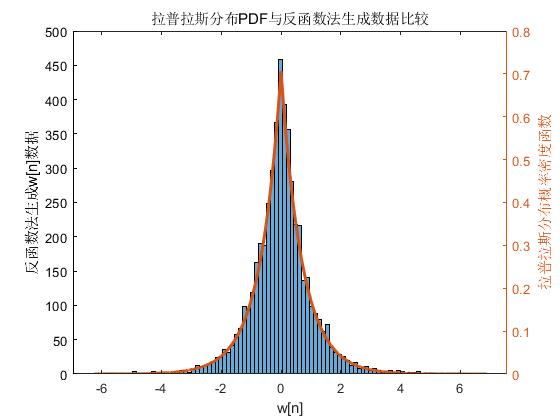
\includegraphics[scale=0.5]{1.jpg}
	\caption{拉普拉斯分布概率密度函数与反函数法生成w[n]数据比较图}
	\label{fig:1}
\end{figure}

样本超过\(3\sigma\)的概率
\begin{align*}
	P\{\vert w[n]\vert >3\sigma\}
	 & =2P\{w[n]<-3\sigma\} \\
	 & =2F(-3\sigma)        \\
	 & =\exp(-3\sqrt{2})    \\
	 & =0.0144
\end{align*}

图\ref*{fig:2}显示了随着样本数N的增大,数据超过\(3\sigma\)的概率变化曲线。可以看到随着样本数N的增加,数据超过\(3\sigma\)的概率逐渐趋于理论值\(\exp(-3\sqrt{2})\)
\begin{figure}[H]
	\centering
	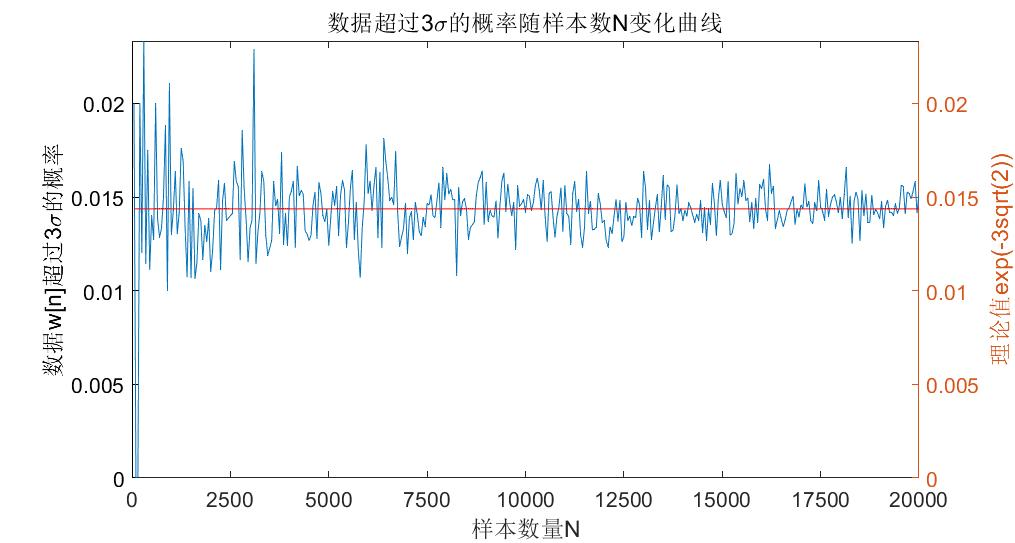
\includegraphics[scale=0.35]{2.jpg}
	\caption{数据超过\(3\sigma\)的概率随数据长度的变化曲线图}
	\label{fig:2}
\end{figure}

\subsubsection*{(2)模拟下式的混合高斯PDF,假定\(\sigma^2_2>\sigma^2_1\)。假定混合高斯平均功率\(\sigma^2\)为1,\(\varepsilon=0.01\),根据不同\(\sigma^2_2,\sigma^2_1\)数值下样本统计分析超过3\(\sigma\)的概率。}
\begin{align*}
	p(n)=(1-\varepsilon)\frac{1}{\sqrt{2\pi \sigma^2_1}}\exp\left(-\frac{n^2}{2\sigma^2_1}\right)+
	\varepsilon \frac{1}{\sqrt{2\pi \sigma^2_2}}\exp\left(-\frac{n^2}{2\sigma^2_2}\right)
\end{align*}

已知混合高斯分布平均功率\(\sigma^2=1\),则\((1-\varepsilon)\sigma^2_1+\varepsilon\sigma^2_2=\sigma^2=1\),所以\(\sigma^2_1=\frac{1-\varepsilon\sigma^2_2}{1-\varepsilon}\),由\(\sigma^2_2>\sigma^2_1\),解得\(\sigma^2_2>1,\sigma^2_1<1\)。

\textbf{1}.首先考虑生成符合高斯分布的随机变量。由于高斯分布的累积分布函数(CDF)\(\Phi(x)\)不是初等函数,它的逆函数无法用解析形式表示,因此高斯分布的随机变量无法用逆变换法产生,但是可以通过Box-Muller变换法产生。

Box-Muller变换法与逆变换法有关。考虑同时构造两个独立的高斯分布的随机变量:随机变量X和Y相互独立,且均服从正态分布,其联合概率密度函数为
\begin{align*}
	f(x,y)
	 & =\frac{1}{\sqrt{2\pi \sigma^2_1}}\exp(-\frac{x}{2\sigma^2_1})\cdot
	\frac{1}{\sqrt{2\pi\sigma^2_1}}\exp(-\frac{y}{2\sigma^2_1})           \\
	 & =\frac{1}{2\pi \sigma^2_1}\exp(-\frac{x^2+y^2}{2\sigma^2_1})
\end{align*}
这个联合概率密度分布的累积分布函数很容易计算,它的积分\(I^2\)是
\begin{align*}
	I^2
	 & =\int \int_{\Omega}\frac{1}{2\pi \sigma^2_1}\exp(-\frac{x^2+y^2}{2\sigma^2_1})dxdy   \\
	 & =\frac{1}{2\pi \sigma^2_1}\int \int_{\Omega}\exp(-\frac{r^2}{2\sigma^2_1})rdrd\theta \\
	 & =\int_{0}^{2\pi}\frac{1}{2\pi}d\theta \cdot
	\int_{0}^{+\infty}\frac{1}{\sigma^2_1}\exp(-\frac{r^2}{2\sigma^2_1})rdr
\end{align*}
积分计算过程中进行了一次从直角坐标系到极坐标系的变换,关于\(\theta\)和r的累积分布函数很容易计算
\begin{align*}
	F_R        & =1-\exp(-\frac{r^2}{2\sigma^2_1}),r\in [0,\infty) \\
	F_{\Theta} & =\frac{\theta}{2\pi },\theta\in [0,2\pi)
\end{align*}

利用逆变换方法,这两个变量\(\Theta\)和\(R\)可以通过两个独立的随机变量\(U_1\sim \mathcal{U}(0,1)\)和\(U_2\sim \mathcal{U}(0,1)\)构造出来

\begin{align*}
	R      & =\sigma_1\sqrt{-2\ln(U_1)} \\
	\Theta & =2\pi U_2
\end{align*}

根据极坐标系到直角坐标系的变换关系
\begin{align*}
	X & =R\cos(\Theta) \\
	Y & =R\sin(\Theta)
\end{align*}
可以得到
\begin{align*}
	X & =\sigma_1\sqrt{-2\ln U_1}\cos(2\pi U_2) \\
	Y & =\sigma_1\sqrt{-2\ln U_1}\sin(2\pi U_2)
\end{align*}
任取X或Y均服从\(\mathcal{N}(0,\sigma^2_1)\)。

同理,若\(U_1^{\prime}\sim \mathcal{U}(0,1),U_2^{\prime}\sim \mathcal{U}(0,1)\),则可以构造出
\begin{align*}
	X^{\prime} & =\sigma_2\sqrt{-2\ln U_1^{\prime}}\cos(2\pi U_2^{\prime}) \\
	Y^{\prime} & =\sigma_2\sqrt{-2\ln U_1^{\prime}}\sin(2\pi U_1^{\prime})
\end{align*}
任取\(X^{\prime}\)或\(Y^{\prime}\)均服从\(\mathcal{N}(0,\sigma^2_2)\)。

\textbf{2}.其次考虑由两个高斯分布的随机变量生成服从混合高斯分布的随机变量。已知混合高斯分布的混合系数分别为\(1-\varepsilon=0.99\)和\(\varepsilon=0.01\),可以从服从\(\mathcal{N}(0,\sigma^2_1)\)和\(\mathcal{N}(0,\sigma^2_2)\)的两个随机变量中以概率0.99和0.01随机选取,就可以得到要求的混合高斯分布。

生成要求的混合高斯分布的算法如下
\begin{algorithm}[H]
	\caption{Gaussian Mixture}
	\label{alg:GMM}
	\begin{algorithmic}[1]
		\REQUIRE \(\sigma_1\ and\ \varepsilon(\varepsilon\in [0,1],\sigma^2_1\in (0,\frac{1}{\varepsilon^2+(1-\varepsilon)^2}))\);
		\ENSURE \(n\);
		\STATE \(U_i\overset{i.i.d}{\sim} \mathcal{U}(0,1),i=1,2,\cdots,5\)
		\STATE \(n_1=\sigma_1\sqrt{-2\ln U_1}\cos(2\pi U_2)\)
		\STATE \(\sigma_2=\frac{1-(1-\varepsilon)\sigma^2_1}{\varepsilon},n_2=\sigma_2\sqrt{-2\ln U_3}\cos(2\pi U_4)\)
		\IF {\(U_5>\varepsilon\)}
		\STATE \(n=n_2\)
		\ELSE
		\STATE \(n=n_1\)
		\ENDIF
		\STATE \textbf{return} \(n\)
	\end{algorithmic}
\end{algorithm}

利用MATLAB编程实现算法\ref*{alg:GMM},得到图\ref*{fig:3}。由于\(\varepsilon=0.01\)时混合高斯分布与单个高斯分布十分相近,难以分辨,所以图\ref*{fig:3}中\(\varepsilon=0.5,\sigma_1^2=0.5,\sigma^2_2=7/4\),数据n长度N为2000。图中直方图代表利用变换法生成的数据n的分布,红色实线代表对应的混合高斯分布的概率密度函数,可以看出生成的数据近似符合混合高斯分布。图中也画出了组成混合高斯分布的单个高斯分布的概率密度函数作为比较,分别为蓝色虚线和绿色虚线。可以求出数据的方差为\(0.9804\approx1\),说明生成的数据符合要求。

\begin{figure}[H]
	\centering
	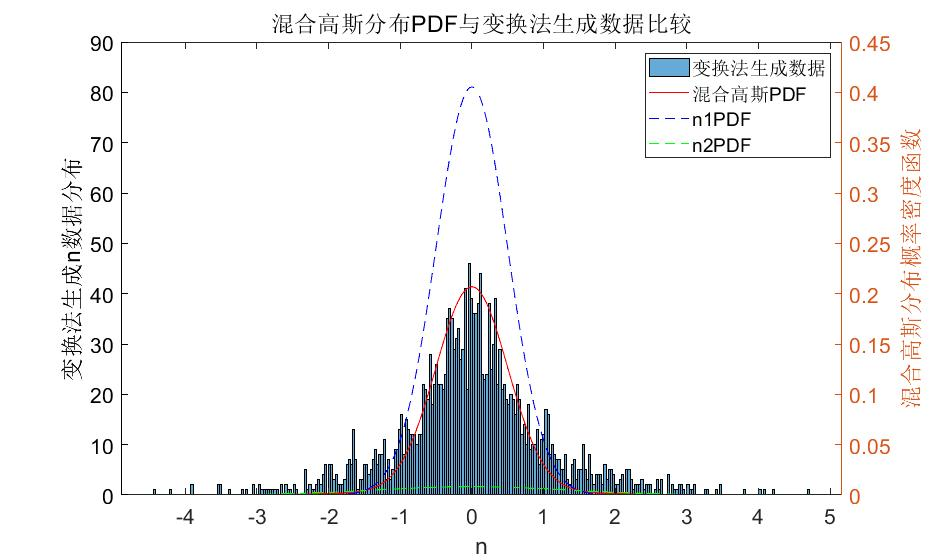
\includegraphics[scale=0.4]{5.jpg}
	\caption{变换法生成数据分布与混合高斯分布比较图}
	\label{fig:3}
\end{figure}

根据算法\ref*{alg:GMM}可以发现,混合高斯分布可以等效为多个高斯分布的加权平均
\begin{align*}
	p(n)=p(n|k=1)P\{k=1\}+p(n|k=2)P\{k=2\}
\end{align*}
其中
\begin{align*}
	P\{k=1\} & =1-\varepsilon                                                             \\
	p(n|k=1) & =\frac{1}{\sqrt{2\pi \sigma^2_1}}\exp\left(-\frac{n^2}{2\sigma^2_1}\right) \\
	P\{k=2\} & =\varepsilon                                                               \\
	p(n|k=2) & =\frac{1}{\sqrt{2\pi \sigma^2_2}}\exp\left(-\frac{n^2}{2\sigma^2_2}\right) \\
\end{align*}
所以混合高斯分布样本超过\(3\sigma\)的概率为多个高斯分布样本超过\(3\sigma\)的概率的加权平均,即
\begin{align*}
	P\{\vert n\vert>3\sigma\}
	 & =P\{k=1\}P\{\vert n_1\vert>3\sigma\}+P\{k=2\}P\{\vert n_2\vert>3\sigma\}                                              \\
	 & =2(1-\varepsilon)\Phi(-\frac{3\sigma}{\sigma_1})+2\varepsilon \Phi(-\frac{3\sigma}{\sigma_2})                         \\
	 & =2(1-\varepsilon)\Phi(-3\sqrt{\frac{(1-\varepsilon)}{1-\varepsilon\sigma_2^2}})+2\varepsilon\Phi(-\frac{3}{\sigma_2})
\end{align*}
其中\(\Phi(x)\)为标准正态分布的累积分布函数。

图\ref*{fig:4}显示了\(\varepsilon=0.01\)时,样本超过\(3\sigma\)的概率随\(\sigma^2_2\)的变化曲线,随着\(\sigma^2_2\)的增长,概率逐渐趋于稳定。

\begin{figure}[H]
	\centering
	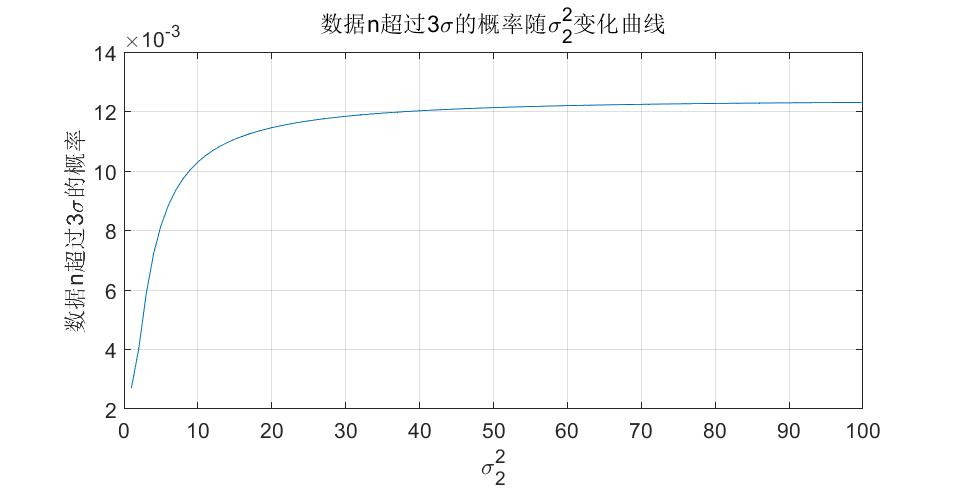
\includegraphics[scale=0.4]{4.jpg}
	\caption{数据超过\(3\sigma\)的概率随\(\sigma^2_2\)的变化曲线图}
	\label{fig:4}
\end{figure}

图\ref*{fig:5}显示了\(\varepsilon=0.01\)时,随着数据长度N的变化,数据超过\(3\sigma\)的概率的变化曲线,这时\(\sigma_1=0.5,\sigma_2=8.6747\),可以发现随着数据长度增长,概率趋于理论值0.0073。

\begin{figure}[H]
	\centering
	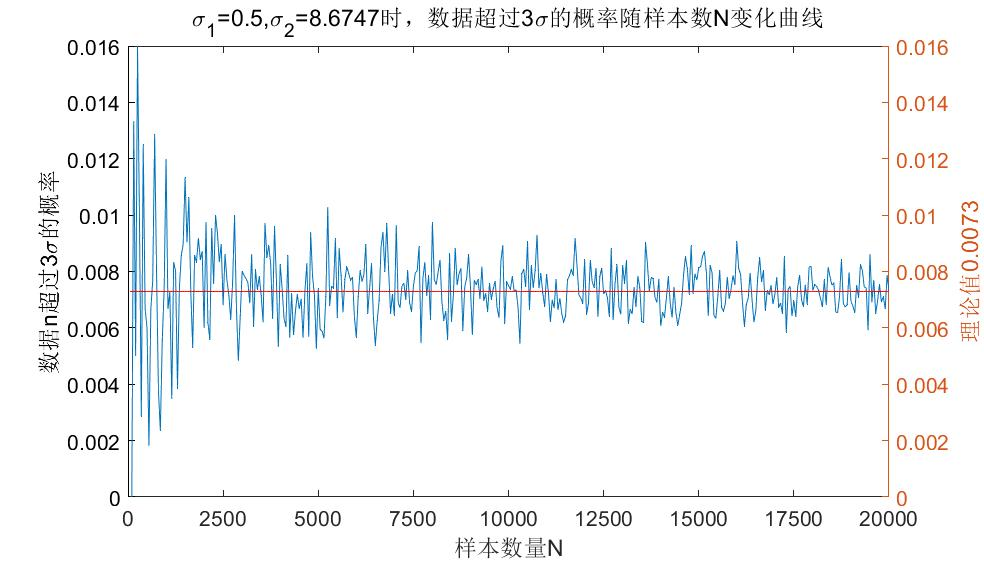
\includegraphics[scale=0.4]{3.jpg}
	\caption{数据超过\(3\sigma\)的概率随数据长度N的变化曲线图}
	\label{fig:5}
\end{figure}

\bibliography{books}
\end{document}